
%% bare_conf.tex
%% V1.3
%% 2007/01/11
%% by Michael Shell
%% See:
%% http://www.michaelshell.org/
%% for current contact information.
%%
%% This is a skeleton file demonstrating the use of IEEEtran.cls
%% (requires IEEEtran.cls version 1.7 or later) with an IEEE conference paper.
%%
%% Support sites:
%% http://www.michaelshell.org/tex/ieeetran/
%% http://www.ctan.org/tex-archive/macros/latex/contrib/IEEEtran/
%% and
%% http://www.ieee.org/

%%*************************************************************************
%% Legal Notice:
%% This code is offered as-is without any warranty either expressed or
%% implied; without even the implied warranty of MERCHANTABILITY or
%% FITNESS FOR A PARTICULAR PURPOSE! 
%% User assumes all risk.
%% In no event shall IEEE or any contributor to this code be liable for
%% any damages or losses, including, but not limited to, incidental,
%% consequential, or any other damages, resulting from the use or misuse
%% of any information contained here.
%%
%% All comments are the opinions of their respective authors and are not
%% necessarily endorsed by the IEEE.
%%
%% This work is distributed under the LaTeX Project Public License (LPPL)
%% ( http://www.latex-project.org/ ) version 1.3, and may be freely used,
%% distributed and modified. A copy of the LPPL, version 1.3, is included
%% in the base LaTeX documentation of all distributions of LaTeX released
%% 2003/12/01 or later.
%% Retain all contribution notices and credits.
%% ** Modified files should be clearly indicated as such, including  **
%% ** renaming them and changing author support contact information. **
%%
%% File list of work: IEEEtran.cls, IEEEtran_HOWTO.pdf, bare_adv.tex,
%%                    bare_conf.tex, bare_jrnl.tex, bare_jrnl_compsoc.tex
%%*************************************************************************

% *** Authors should verify (and, if needed, correct) their LaTeX system  ***
% *** with the testflow diagnostic prior to trusting their LaTeX platform ***
% *** with production work. IEEE's font choices can trigger bugs that do  ***
% *** not appear when using other class files.                            ***
% The testflow support page is at:
% http://www.michaelshell.org/tex/testflow/



% Note that the a4paper option is mainly intended so that authors in
% countries using A4 can easily print to A4 and see how their papers will
% look in print - the typesetting of the document will not typically be
% affected with changes in paper size (but the bottom and side margins will).
% Use the testflow package mentioned above to verify correct handling of
% both paper sizes by the user's LaTeX system.
%
% Also note that the "draftcls" or "draftclsnofoot", not "draft", option
% should be used if it is desired that the figures are to be displayed in
% draft mode.
%
\documentclass[10pt, conference, compsocconf]{IEEEtran}
% Add the compsocconf option for Computer Society conferences.
%
% If IEEEtran.cls has not been installed into the LaTeX system files,
% manually specify the path to it like:
% \documentclass[conference]{../sty/IEEEtran}





% Some very useful LaTeX packages include:
% (uncomment the ones you want to load)


% *** MISC UTILITY PACKAGES ***
%
%\usepackage{ifpdf}
% Heiko Oberdiek's ifpdf.sty is very useful if you need conditional
% compilation based on whether the output is pdf or dvi.
% usage:
% \ifpdf
%   % pdf code
% \else
%   % dvi code
% \fi
% The latest version of ifpdf.sty can be obtained from:
% http://www.ctan.org/tex-archive/macros/latex/contrib/oberdiek/
% Also, note that IEEEtran.cls V1.7 and later provides a builtin
% \ifCLASSINFOpdf conditional that works the same way.
% When switching from latex to pdflatex and vice-versa, the compiler may
% have to be run twice to clear warning/error messages.






% *** CITATION PACKAGES ***
%
%\usepackage{cite}
% cite.sty was written by Donald Arseneau
% V1.6 and later of IEEEtran pre-defines the format of the cite.sty package
% \cite{} output to follow that of IEEE. Loading the cite package will
% result in citation numbers being automatically sorted and properly
% "compressed/ranged". e.g., [1], [9], [2], [7], [5], [6] without using
% cite.sty will become [1], [2], [5]--[7], [9] using cite.sty. cite.sty's
% \cite will automatically add leading space, if needed. Use cite.sty's
% noadjust option (cite.sty V3.8 and later) if you want to turn this off.
% cite.sty is already installed on most LaTeX systems. Be sure and use
% version 4.0 (2003-05-27) and later if using hyperref.sty. cite.sty does
% not currently provide for hyperlinked citations.
% The latest version can be obtained at:
% http://www.ctan.org/tex-archive/macros/latex/contrib/cite/
% The documentation is contained in the cite.sty file itself.






% *** GRAPHICS RELATED PACKAGES ***
%
\ifCLASSINFOpdf
  % \usepackage[pdftex]{graphicx}
  % declare the path(s) where your graphic files are
  % \graphicspath{{../pdf/}{../jpeg/}}
  % and their extensions so you won't have to specify these with
  % every instance of \includegraphics
  % \DeclareGraphicsExtensions{.pdf,.jpeg,.png}
\else
  % or other class option (dvipsone, dvipdf, if not using dvips). graphicx
  % will default to the driver specified in the system graphics.cfg if no
  % driver is specified.
  % \usepackage[dvips]{graphicx}
  % declare the path(s) where your graphic files are
  % \graphicspath{{../eps/}}
  % and their extensions so you won't have to specify these with
  % every instance of \includegraphics
  % \DeclareGraphicsExtensions{.eps}
\fi
% graphicx was written by David Carlisle and Sebastian Rahtz. It is
% required if you want graphics, photos, etc. graphicx.sty is already
% installed on most LaTeX systems. The latest version and documentation can
% be obtained at: 
% http://www.ctan.org/tex-archive/macros/latex/required/graphics/
% Another good source of documentation is "Using Imported Graphics in
% LaTeX2e" by Keith Reckdahl which can be found as epslatex.ps or
% epslatex.pdf at: http://www.ctan.org/tex-archive/info/
%
% latex, and pdflatex in dvi mode, support graphics in encapsulated
% postscript (.eps) format. pdflatex in pdf mode supports graphics
% in .pdf, .jpeg, .png and .mps (metapost) formats. Users should ensure
% that all non-photo figures use a vector format (.eps, .pdf, .mps) and
% not a bitmapped formats (.jpeg, .png). IEEE frowns on bitmapped formats
% which can result in "jaggedy"/blurry rendering of lines and letters as
% well as large increases in file sizes.
%
% You can find documentation about the pdfTeX application at:
% http://www.tug.org/applications/pdftex





% *** MATH PACKAGES ***
%
%\usepackage[cmex10]{amsmath}
% A popular package from the American Mathematical Society that provides
% many useful and powerful commands for dealing with mathematics. If using
% it, be sure to load this package with the cmex10 option to ensure that
% only type 1 fonts will utilized at all point sizes. Without this option,
% it is possible that some math symbols, particularly those within
% footnotes, will be rendered in bitmap form which will result in a
% document that can not be IEEE Xplore compliant!
%
% Also, note that the amsmath package sets \interdisplaylinepenalty to 10000
% thus preventing page breaks from occurring within multiline equations. Use:
%\interdisplaylinepenalty=2500
% after loading amsmath to restore such page breaks as IEEEtran.cls normally
% does. amsmath.sty is already installed on most LaTeX systems. The latest
% version and documentation can be obtained at:
% http://www.ctan.org/tex-archive/macros/latex/required/amslatex/math/





% *** SPECIALIZED LIST PACKAGES ***
%
%\usepackage{algorithmic}
% algorithmic.sty was written by Peter Williams and Rogerio Brito.
% This package provides an algorithmic environment fo describing algorithms.
% You can use the algorithmic environment in-text or within a figure
% environment to provide for a floating algorithm. Do NOT use the algorithm
% floating environment provided by algorithm.sty (by the same authors) or
% algorithm2e.sty (by Christophe Fiorio) as IEEE does not use dedicated
% algorithm float types and packages that provide these will not provide
% correct IEEE style captions. The latest version and documentation of
% algorithmic.sty can be obtained at:
% http://www.ctan.org/tex-archive/macros/latex/contrib/algorithms/
% There is also a support site at:
% http://algorithms.berlios.de/index.html
% Also of interest may be the (relatively newer and more customizable)
% algorithmicx.sty package by Szasz Janos:
% http://www.ctan.org/tex-archive/macros/latex/contrib/algorithmicx/




% *** ALIGNMENT PACKAGES ***
%
%\usepackage{array}
% Frank Mittelbach's and David Carlisle's array.sty patches and improves
% the standard LaTeX2e array and tabular environments to provide better
% appearance and additional user controls. As the default LaTeX2e table
% generation code is lacking to the point of almost being broken with
% respect to the quality of the end results, all users are strongly
% advised to use an enhanced (at the very least that provided by array.sty)
% set of table tools. array.sty is already installed on most systems. The
% latest version and documentation can be obtained at:
% http://www.ctan.org/tex-archive/macros/latex/required/tools/


%\usepackage{mdwmath}
%\usepackage{mdwtab}
% Also highly recommended is Mark Wooding's extremely powerful MDW tools,
% especially mdwmath.sty and mdwtab.sty which are used to format equations
% and tables, respectively. The MDWtools set is already installed on most
% LaTeX systems. The lastest version and documentation is available at:
% http://www.ctan.org/tex-archive/macros/latex/contrib/mdwtools/


% IEEEtran contains the IEEEeqnarray family of commands that can be used to
% generate multiline equations as well as matrices, tables, etc., of high
% quality.

\usepackage[ruled,linesnumbered,lined]{algorithm2e}

%\usepackage{amsmath}
%\usepackage{enumitem}
%\usepackage{eqparbox}
% Also of notable interest is Scott Pakin's eqparbox package for creating
% (automatically sized) equal width boxes - aka "natural width parboxes".
% Available at:
% http://www.ctan.org/tex-archive/macros/latex/contrib/eqparbox/

\usepackage{graphicx}
\usepackage{subfigure}
\graphicspath{{figure/}}

\usepackage{hyperref}
\usepackage{multirow}
\usepackage{balance}
\usepackage{comment}
\usepackage{tikz}
\usepackage[numbers,sort&compress]{natbib}

\usepackage{color}
\definecolor{dkgreen}{rgb}{0,0.6,0}
\definecolor{gray}{rgb}{0.5,0.5,0.5}
\definecolor{mauve}{rgb}{0.58,0,0.82}
% Default settings for code listings

\newcommand{\tabincell}[2]{\begin{tabular}{@{}#1@{}}#2\end{tabular}}

\def\sharedaffiliation{
\end{tabular}
\begin{tabular}{c}}

% *** SUBFIGURE PACKAGES ***
%\usepackage[tight,footnotesize]{subfigure}
% subfigure.sty was written by Steven Douglas Cochran. This package makes it
% easy to put subfigures in your figures. e.g., "Figure 1a and 1b". For IEEE
% work, it is a good idea to load it with the tight package option to reduce
% the amount of white space around the subfigures. subfigure.sty is already
% installed on most LaTeX systems. The latest version and documentation can
% be obtained at:
% http://www.ctan.org/tex-archive/obsolete/macros/latex/contrib/subfigure/
% subfigure.sty has been superceeded by subfig.sty.

%\usepackage[caption=false]{caption}
%\usepackage[font=footnotesize]{subfig}
% subfig.sty, also written by Steven Douglas Cochran, is the modern
% replacement for subfigure.sty. However, subfig.sty requires and
% automatically loads Axel Sommerfeldt's caption.sty which will override
% IEEEtran.cls handling of captions and this will result in nonIEEE style
% figure/table captions. To prevent this problem, be sure and preload
% caption.sty with its "caption=false" package option. This is will preserve
% IEEEtran.cls handing of captions. Version 1.3 (2005/06/28) and later 
% (recommended due to many improvements over 1.2) of subfig.sty supports
% the caption=false option directly:
%\usepackage[caption=false,font=footnotesize]{subfig}
%
% The latest version and documentation can be obtained at:
% http://www.ctan.org/tex-archive/macros/latex/contrib/subfig/
% The latest version and documentation of caption.sty can be obtained at:
% http://www.ctan.org/tex-archive/macros/latex/contrib/caption/




% *** FLOAT PACKAGES ***
%
%\usepackage{fixltx2e}
% fixltx2e, the successor to the earlier fix2col.sty, was written by
% Frank Mittelbach and David Carlisle. This package corrects a few problems
% in the LaTeX2e kernel, the most notable of which is that in current
% LaTeX2e releases, the ordering of single and double column floats is not
% guaranteed to be preserved. Thus, an unpatched LaTeX2e can allow a
% single column figure to be placed prior to an earlier double column
% figure. The latest version and documentation can be found at:
% http://www.ctan.org/tex-archive/macros/latex/base/



%\usepackage{stfloats}
% stfloats.sty was written by Sigitas Tolusis. This package gives LaTeX2e
% the ability to do double column floats at the bottom of the page as well
% as the top. (e.g., "\begin{figure*}[!b]" is not normally possible in
% LaTeX2e). It also provides a command:
%\fnbelowfloat
% to enable the placement of footnotes below bottom floats (the standard
% LaTeX2e kernel puts them above bottom floats). This is an invasive package
% which rewrites many portions of the LaTeX2e float routines. It may not work
% with other packages that modify the LaTeX2e float routines. The latest
% version and documentation can be obtained at:
% http://www.ctan.org/tex-archive/macros/latex/contrib/sttools/
% Documentation is contained in the stfloats.sty comments as well as in the
% presfull.pdf file. Do not use the stfloats baselinefloat ability as IEEE
% does not allow \baselineskip to stretch. Authors submitting work to the
% IEEE should note that IEEE rarely uses double column equations and
% that authors should try to avoid such use. Do not be tempted to use the
% cuted.sty or midfloat.sty packages (also by Sigitas Tolusis) as IEEE does
% not format its papers in such ways.





% *** PDF, URL AND HYPERLINK PACKAGES ***
%
%\usepackage{url}
% url.sty was written by Donald Arseneau. It provides better support for
% handling and breaking URLs. url.sty is already installed on most LaTeX
% systems. The latest version can be obtained at:
% http://www.ctan.org/tex-archive/macros/latex/contrib/misc/
% Read the url.sty source comments for usage information. Basically,
% \url{my_url_here}.





% *** Do not adjust lengths that control margins, column widths, etc. ***
% *** Do not use packages that alter fonts (such as pslatex).         ***
% There should be no need to do such things with IEEEtran.cls V1.6 and later.
% (Unless specifically asked to do so by the journal or conference you plan
% to submit to, of course. )


% correct bad hyphenation here
\hyphenation{op-tical net-works semi-conduc-tor}


\begin{document}
%
% paper title
% can use linebreaks \\ within to get better formatting as desired
\title{MURS: Mitigating Memory Pressure in Data Processing Systems for Service}


% author names and affiliations
% use a multiple column layout for up to two different
% affiliations

\author{\IEEEauthorblockN{Xiong Zhang, Xuanhua Shi, Hai Jin, Song Wu, Zhixiang Ke}
\IEEEauthorblockA{Services Computing Technology and System Lab\\
Cluster and Grid Computing Lab\\
Big Data Technology and System Lab\\
School of Computer Science and Technology\\
Huazhong University of Science and Technology, Wuhan, 430074, China\\
Email: \{wxzhang, xhshi, hjin, wusong, zhxke\}@hust.edu.cn}
}

% conference papers do not typically use \thanks and this command
% is locked out in conference mode. If really needed, such as for
% the acknowledgment of grants, issue a \IEEEoverridecommandlockouts
% after \documentclass

% for over three affiliations, or if they all won't fit within the width
% of the page, use this alternative format:
% 
%\author{\IEEEauthorblockN{Michael Shell\IEEEauthorrefmark{1},
%Homer Simpson\IEEEauthorrefmark{2},
%James Kirk\IEEEauthorrefmark{3}, 
%Montgomery Scott\IEEEauthorrefmark{3} and
%Eldon Tyrell\IEEEauthorrefmark{4}}
%\IEEEauthorblockA{\IEEEauthorrefmark{1}School of Electrical and Computer Engineering\\
%Georgia Institute of Technology,
%Atlanta, Georgia 30332--0250\\ Email: see http://www.michaelshell.org/contact.html}
%\IEEEauthorblockA{\IEEEauthorrefmark{2}Twentieth Century Fox, Springfield, USA\\
%Email: homer@thesimpsons.com}
%\IEEEauthorblockA{\IEEEauthorrefmark{3}Starfleet Academy, San Francisco, California 96678-2391\\
%Telephone: (800) 555--1212, Fax: (888) 555--1212}
%\IEEEauthorblockA{\IEEEauthorrefmark{4}Tyrell Inc., 123 Replicant Street, Los Angeles, California 90210--4321}}




% use for special paper notices
%\IEEEspecialpapernotice{(Invited Paper)}




% make the title area
\maketitle


\begin{abstract}
%In-memory computing systems are shown to suffer serious memory pressure as well as they are for service, the memory pressure will effect all submitted jobs. Memory pressure is coming from the running tasks as they produce massive long-lived data objects in limited memory, which brings significant memory and CPU overheads. Some tasks result in heavy memory pressure because of the operations and dataset they process, which affects all running tasks in the system. We find that each task includes several function APIs provided by the framework, and most function APIs produce long-lived data objects in memory within their own regular models; some need constant memory space while some need linear memory space. As different models have different impact on memory pressure, we propose memory usage rate to classify which model a task belongs to. Based on the memory usage rate, we design a scheduler called MURS to schedule all running tasks and mitigate heavy memory pressure. We implement MURS in Spark and the experimental study shows that, when compare to Spark, our scheduler can 1) decrease the execution time of submitted job by up to 65.8\%; 2) mitigate the memory pressure in server by decreasing the garbage collection time by up to 81\%; and 3) avoid about 90\% of spill tasks to reduce disk I/O.

It has been shown that in-memory computing systems suffer from serious memory pressure. The memory pressure will affect all submitted jobs. Memory pressure comes from the running tasks as they produce massive long-living data objects in the limited memory space. The long-living objects incur significant memory and CPU overheads. Some tasks cause the heavy memory pressure because of the operations and dataset they process, which in turn affect all running tasks in the system. Our studies show that a task often call several API functions provided by the need to constant memory space, while some need the linear memory space. As different models have different impact on memory pressure, we propose a method of classifying the models that the tasks belong to. The method uses the memory usage rate as the classification criteria. Further, we design a scheduler called MURS to mitigate the memory pressure. We implement MURS in Spark and conduct the experiments to evaluate the performance of MURS. The results show that when comparing to Spark, our scheduler can 1) decrease the execution time of submitted jobs by up to 65.8\%, 2) mitigate the memory pressure in the server by decreasing the garbage collection time by up to 81\%, and 3) reduce the data spilling, and hence disk I/Os, by approximately 90\%.

\end{abstract}

\begin{IEEEkeywords}
memory pressure; memory usage rate; task scheduler; data processing systems for service

\end{IEEEkeywords}


% For peer review papers, you can put extra information on the cover
% page as needed:
% \ifCLASSOPTIONpeerreview
% \begin{center} \bfseries EDICS Category: 3-BBND \end{center}
% \fi
%
% For peerreview papers, this IEEEtran command inserts a page break and
% creates the second title. It will be ignored for other modes.
\IEEEpeerreviewmaketitle

\section{Introduction}

Background(一段) 

\begin{itemize}
\item 1. GPU性能评估的重要性;
\item 2. GPU性能评估需要考虑的问题,准确性,指导性等等。
\end{itemize}

Motivation(一段) 

\begin{itemize}
\item 1. 监控工具可以监控的指标有非常多种,需要熟练的技术知识才能分析这些指标;
\item 2. 指标太多不利于直接发现最关键的性能瓶颈,
需要一定的经验知识作为辅导;
\item 3. 数学模型的建立有助于评估性能,但是精确的模型的建立及理解都很困难,对模型建立者和使用者都需要对GPU架构有深刻理解。
\end{itemize}

Introduction(两段) 

监控工具得到的指标非常多,往往一个指标或者多个指标集可以指向一个具体的性能问题。而不同的GPU程序又必然有一个影响最大的性能瓶颈。所以能够快速定位影响最大的性能瓶颈非常关键。决策树的分析模型是机器学习中基于信息论的分类模型,更加专注于信息对整个数据集的影响,因此由决策树决定需要考虑的指标,非常适合解决该问题。

获取影响最大的指标集后,极大地缩小了需要考虑的范围。如果继续采用决策树的分类性能瓶颈和优化方案具有一定的误差,这与机器学习特性有关。传统的数学模型准确度往往比机器学习算法准确率要高,由于需要考虑的指标集已经很小了,因此通过理论模型分析这些指标更为恰当。分析方法从三个层面考虑:应用层面(包括应用在计算需求、数据排列上的处理),系统层面(包括指令调度、资源管理和分配等),硬件层面(包括通信带宽、资源特性等)。结合小范围的数据集和三个层面,本文模型可以快速定位并准确提出性能瓶颈与优化方案。

Contribution(三点) 

\begin{itemize}
\item 1. 提供了一种结合决策树模型和理论分析模型的GPU应用性能分析模型,可以更加准确地定位性能瓶颈并提出优化方案。
\item 2. 提供了一种基于决策树的分析算法,在GPU应用程序的监控数据中,由决策树决定影响最大的指标集并做进一步的理论分析。决策树的方法可以快速地决策GPU应用程序的瓶颈,缩小需要考虑和分析的范围。决策树不仅基于microbenchmark,还可以基于上层数据处理系统的benchmark训练,适用范围广。
\item 3. 基于决策树的分析结果,提出了面向应用、系统和硬件的三层理论分析模型,进一步定位决策树得出的瓶颈结果。理论分析模型可以在小范围内更加准确地确定GPU应用瓶颈并提出优化方法。
\end{itemize}

Paper(一段) 

第II章,相关工作;第III章:背景;第IV章,决策树;第V章,分析模型;第VI章,实验;第VII章,结论。
\section{Motivation}
\label{sec:motivation}

Memory is a critical type of resource in current data processing systems, especially in the in-memory computing systems~\cite{shi:mammoth}. However, limited memory space leads to memory pressure and can cause frequent garbage collection or out-of-memory errors~\cite{fang2015interruptible}, both of which seriously affect the performance of the data processing system. A data processing system is often deployed as a service. To understand the impact of memory pressure on the data processing systems and identify the cause of inefficiency, we investigate the running of the tasks with different memory requirements. We choose two types of applications, PageRank(PR) and WordCount(WC), which are the common benchmarks in Spark. The input dataset of PR and WC are webbase-2001 (30GB) and HiBench Random Writer (50GB). As a data processing system, Spark can also work as a server through Spark Job Server. We first run the tasks in the service mode, in which we submit PR and WC simultaneously to the Spark server and run them with a fair scheduler in Spark. As a comparison, we also run PR and WC in the batch mode, in which PR and WC are processed one after the other. We record the execution times and garbage collections times of all tasks under these two modes, which are plotted in Figure~\ref{fig:memorypressure}. We then analyze the memory pressure through the results. 

%Memory is an important resource in current data processing systems, especially in these in-memory computing systems~\cite{shi:mammoth}. Limited memory space will result in memory pressure. The impact of memory pressure can be frequent garbage collection~\cite{lulu:deca} or out of memory error~\cite{fang2015interruptible}, both have serious effect on the data processing system. We can evaluate the memory pressure by PageRank(PR) and WordCount(WC), two common benchmarks, in Spark. The details of clusters and applications are shown in the evaluation. Spark can work for service by Spark Job Server. We firstly run PR and WC individually in batch processing to evaluate the memory pressure themselves, and then evaluate the memory pressure in Spark for service by submitting them together to Spark Job Server. In each stage, we count the medium of execution time and garbage collection time of all tasks, as shown in Figure~\ref{fig:memorypressure}.

\begin{figure}[!t]
\centering
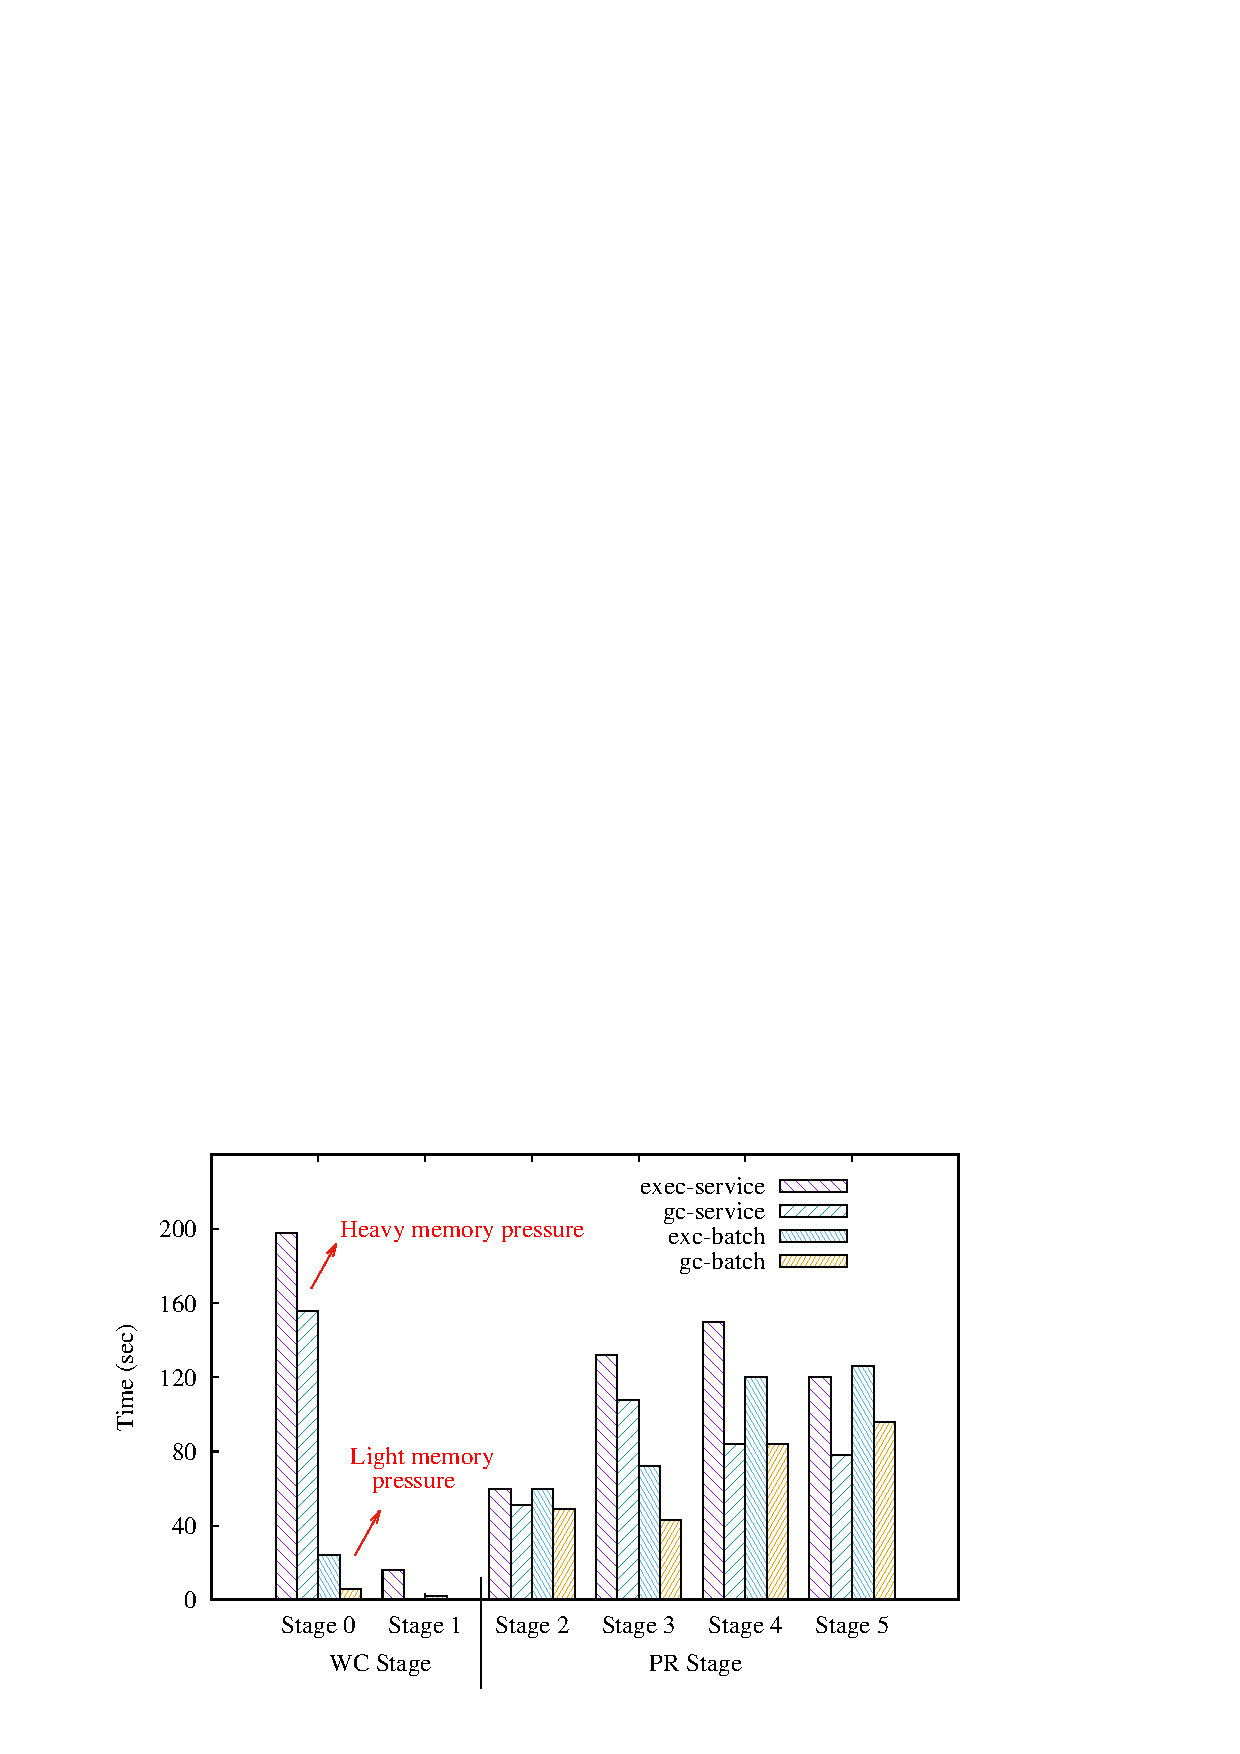
\includegraphics[width=0.4\textwidth]{motivation-exec-gc.pdf}
\vspace{-2mm}
\caption{WC suffers memory pressure from PR}
\vspace{-6mm}
\label{fig:memorypressure}
\end{figure}

\begin{comment}
\begin{figure}[!t]
\centering
\subfigure[Execution Time]{
\label{fig:subfig:mot-exec}
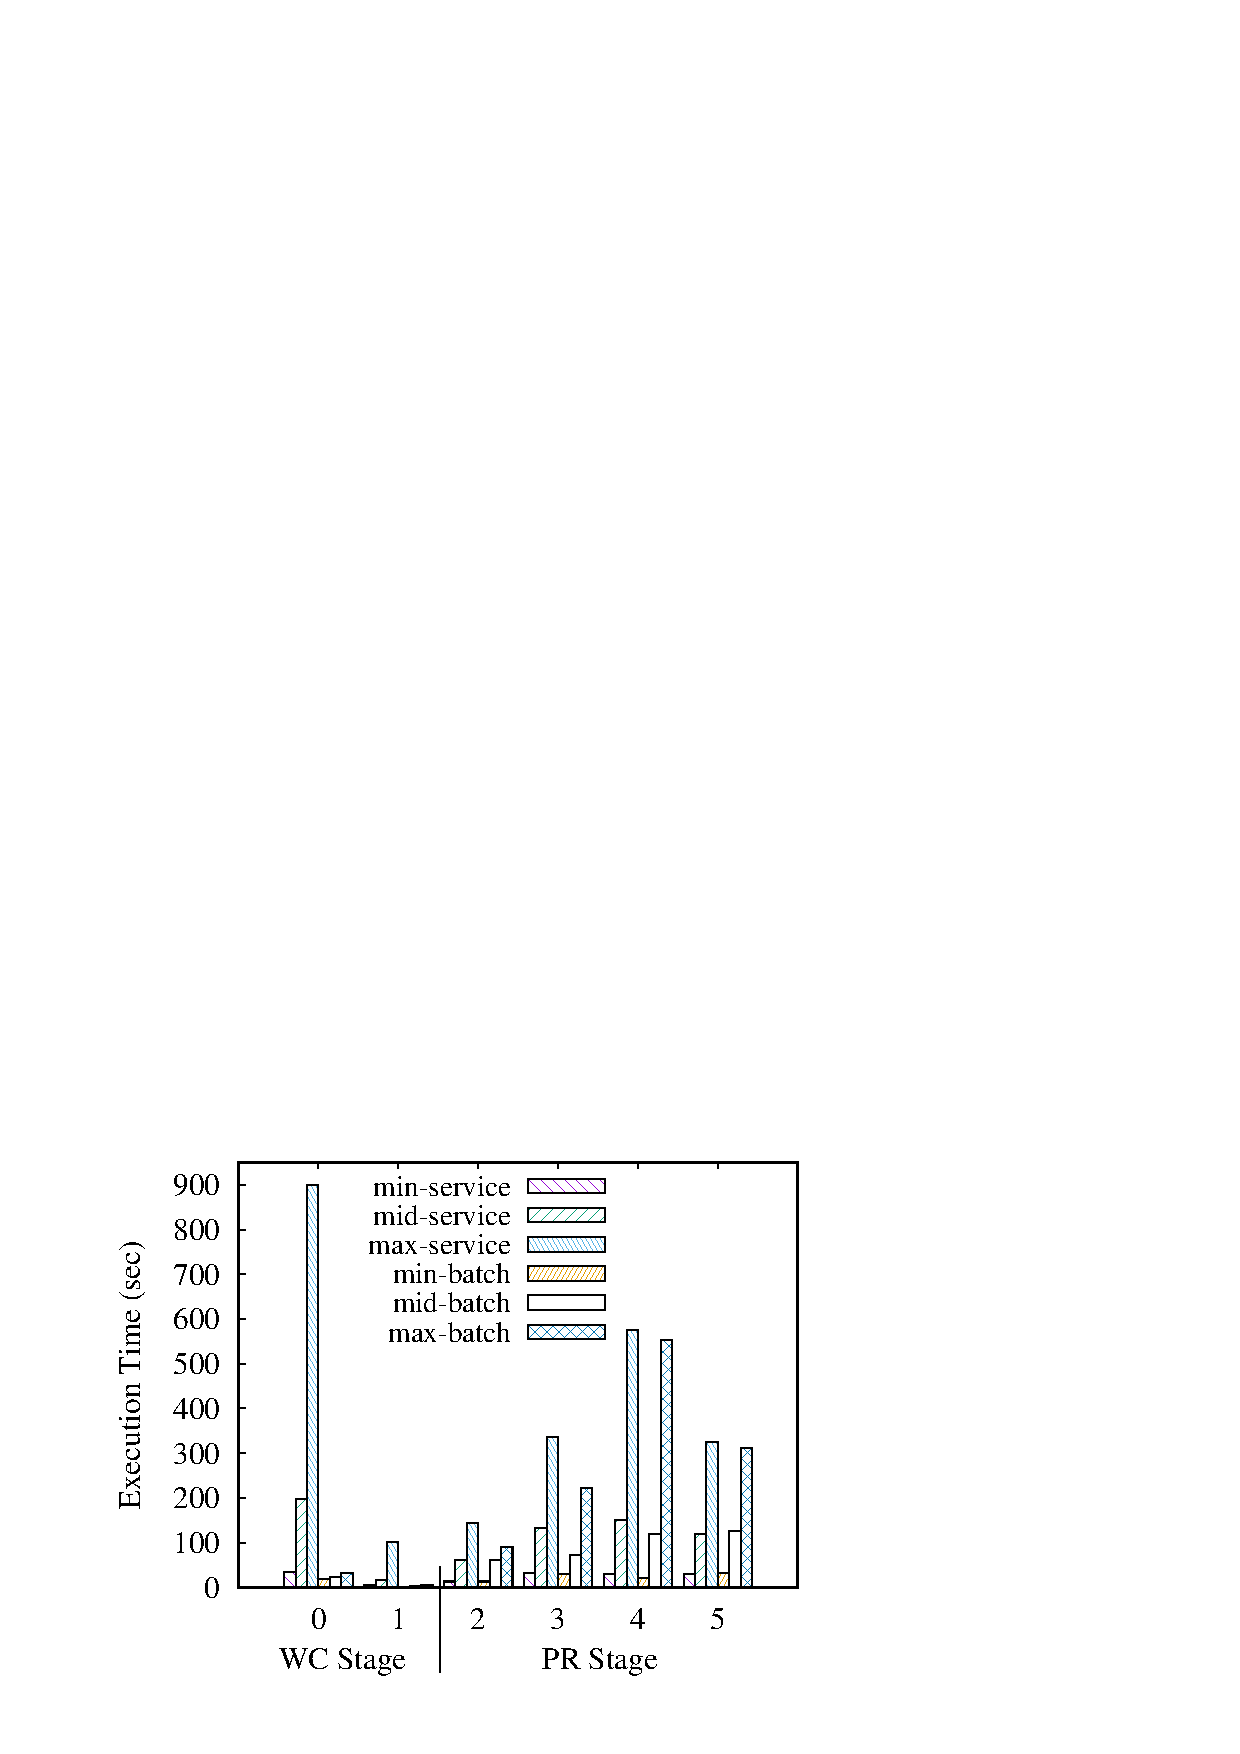
\includegraphics[width=0.231\textwidth]{motivation-exec.pdf}}
\hspace{-1.3ex}
\subfigure[GC Time]{
\label{fig:subfig:mot-gc}
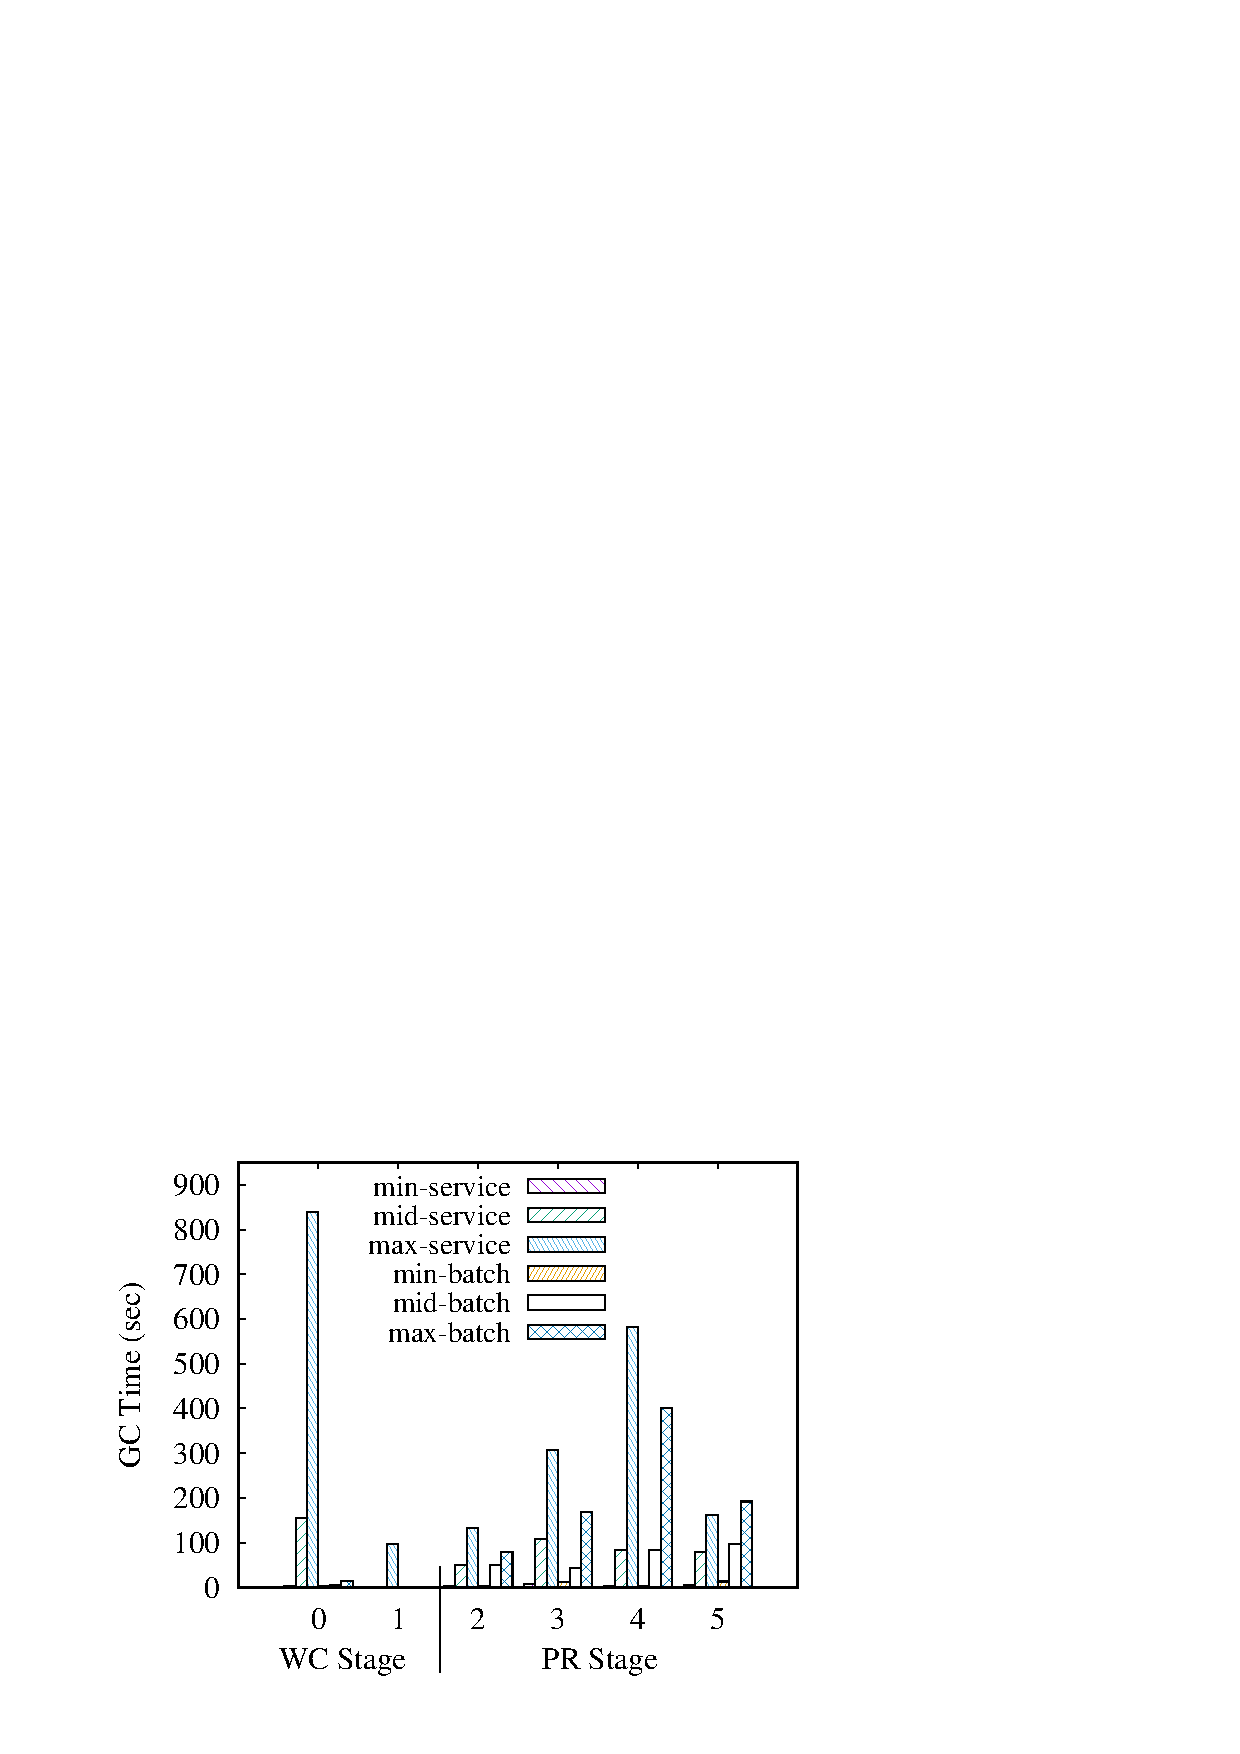
\includegraphics[width=0.231\textwidth]{motivation-gc.pdf}}
\label{fig:wc-result}
\vspace{-2mm}
\caption{The Impact of Memory Pressure}
\vspace{-2mm}
\end{figure}
\end{comment}

%Some applications, such as PR in our observation, they cache intermediate data in memory and iteratively computes the result; one iteration means a stage in Spark. Because the caching data is alive as long as the job, memory space becomes not enough for computation, which means the memory pressure is heavy in PR. However, compare with the PR, WC is another type of task, in which contains only some simple operations, just two stages and very small intermediate shuffle data--though the input data is larger than PR. Furthermore, both the execution time and garbage collection time are low in WC, and the memory pressure is much lighter than PR. The result of PR in batch processing verifies memory pressure and heavy garbage collection (exec-batch and gc-batch in Figure~\ref{fig:memorypressure}). As we can see, the garbage collection time in task accounts for a very great proportion of the execution time.

We observe that PR caches intermediate data in memory and iteratively compute the result. One iteration corresponds to one stage in Spark. Because the caching data is alive as long as the job itself, the memory space becomes gradually less and the task computation will suffer. If this occurs, it indicates the memory pressure caused by PR is heavy. Compare with PR, however, WC only contains some simple operations. WC has only two processing stages and during its execution, a very small amount of intermediate shuffle data are generated (although the input data of WC is larger than that of PR). Furthermore, both the execution time and garbage collection time are low in WC, and the memory pressure is much lighter than PR. The result of PR in the batch mode also verifies its high memory pressure and heavy garbage collection which are the results labelled as exec-batch and gc-batch in Figure~\ref{fig:memorypressure}. As we can see, the garbage collection time accounts for a very large proportion of the execution time.

%PR caches some intermediate data in memory and iteratively computes the result, each iteration means a stage in Spark. The caching data is lived as long as the job, thus available memory space for computation is less which means the memory pressure in PR is heavy. The result of PR in batch processing proves the memory pressure and heavy garbage collection (exec-batch and gc-batch in Figure~\ref{fig:memorypressure}). The garbage collection time in one task has a heavy part in the execution time. However, WC just contains some simple operations and two stages, and the intermediate shuffle data is small although the input data is larger than PR. The memory pressure in WC is light, both the execution time and the garbage collection time is low.

When multiple jobs, such as PR and WC, are submitted to and run by the Spark 
service simultaneously, the jobs are run with a fair scheduler provided by Spark. 
Although WC has much more light memory pressure than PR, all running tasks  
suffer from the heavy memory pressure produced by PR. We find that the execution time 
(exec-service in Figure~\ref{fig:memorypressure} of every task in each stage of PR has little change, except some maximum execution times. This is because 
almost all memory pressure comes from PR and therefore the executions of PR in the service mode and the batch mode show similar trends. However, the execution of WC in the service mode is very different from that in the batch mode. This is because in the service mode, both applications are run simultaneously and therefore WC suffers from the memory pressure produced by PR even if WC is a
light task itself. In the batch mode, since the applications are run one after another. The high memory pressure created by PR will not affect the running of WC.

%If PR and WC are submitted to Spark service, the submitted jobs will run with fair scheduler (provided by Spark). Although PR suffer memory pressure and WC has light memory pressure, all running tasks must suffer the heavy memory pressure produced by PR. We find that the execution time (exec-service in Figure~\ref{fig:memorypressure}) of each task in each stage has a little change in PR except some maximum values. The reason is that almost all memory pressure is coming form PR, running in Spark for service and batch processing is similar. However, WC must suffer the memory pressure produced by PR. The execution time of WC in the first stage has large fluctuation compared to that in batch processing. And we find that the extended time is almost all come from the memory pressure.

In summary, our results implicate that in a system of the service mode, 1) the heavy memory pressure will result in frequent garbage collection, which consumes most of the time and reduce the throughput; 2) the light tasks suffer from heavy memory pressure produced by the heavy tasks; and 3) the heavy tasks obtain the resources later because these resources are occupied chronically by light tasks, and the heavy tasks themselves are the source of memory pressure.

By observing the first stage of PR and WC, we discover that the tasks of PR and WC invoke different function APIs, which determine the impact of each task on memory pressure. If we can identify and classify these tasks by the characteristics of the function APIs, we can suspend the heavy tasks and leave adequate memory space to the light tasks when the memory pressure show up. This can improve the throughput of the service-mode systems and allow all tasks to run with enough memory space and hence light memory pressure.

%Focus on the first stage of PR and WC, we discover that running tasks in PR and WC execute different function APIs. This determines the impact of each task on memory pressure. If we can identify and classify these tasks by the characteristics of function APIs implemented, while the memory pressure comes, we can suspend the heavy tasks and leave enough memory space for the light tasks. This will ensure the throughput of the system for service, and allow all tasks to run with enough memory space and without heavy memory pressure. 

%From the evaluation, we can find that when system is for service, 1) the heavy memory pressure will result in frequent garbage collection which consume most time to cut the throughput. 2) tasks with light memory pressure must suffer the heavy memory pressure produced by others. 3) tasks with heavy memory pressure will get resources later because these resources are occupied longer by these tasks with light memory pressure, and the source of memory pressure is themselves. If we can classify these tasks, when the memory pressure comes, we can stop these tasks which result in heavy memory pressure and remain enough memory space for these tasks which result in light memory pressure. It will ensure the throughput of system for service, and all tasks can run with enough memory space and without heavy memory pressure.  

%While 33\% space are cached data objects that occupy the space with long lifetime, garbage collection will not reclaim these space. We get the cost time and reclaimed space of garbage collection in Figure~\ref{fig:memorypressure}. First, the garbage collections are very frequent and the throughput of job is only 35.7\%. This proves that memory pressure is heavy in the system. Second, the cost of each garbage collection is expensive (GC Time is high in the figure). Some garbage collections which are called full GC will stop the world to mark and clean all the heap. Full GC occurs frequently because the number of lived data objects in memory is too large, it cost more time to mark the lived data objects. Too much lived data objects means less space reclaimed in each garbage collection. Thus, when less space is reclaimed (Reclaimed Space is low in the figure), more time will the garbage collection cost. The worst case is that, frequent garbage collections and less reclaimed space will hinder the performance into the vicious circle.

%Multi-tenant service is provided with the same configurations, we use WordCount, another benchmark in Spark, to balance the execution of PageRank. The dataset of WordCount is produced by HiBench~\cite{www:hibench} and the size is 50GB. The memory usage and garbage collection are the same as the batch processing. %We then consider the completion time with fair scheduler as shown in Figure~\ref{fig:memorypressure2}.
%WC has no cached data, thus memory pressure in WC is lighter and the execution time of WC can be less. However, at first, executors will be lost when jobs are submitted without any configurations tuning. The heavy memory pressure influences the output of disk and network which result in the loss of heartbeat of executors. Second, after the tuning of shuffle configurations, the throughput of WC decreases to 20\%. These tasks without producing much memory pressure must suffer the serious memory pressure from other tenants. %On the other side, PR can also benefit from WC because there are less memory pressure compared to processing batch.

\begin{comment}
\begin{figure}[!t]
\centering
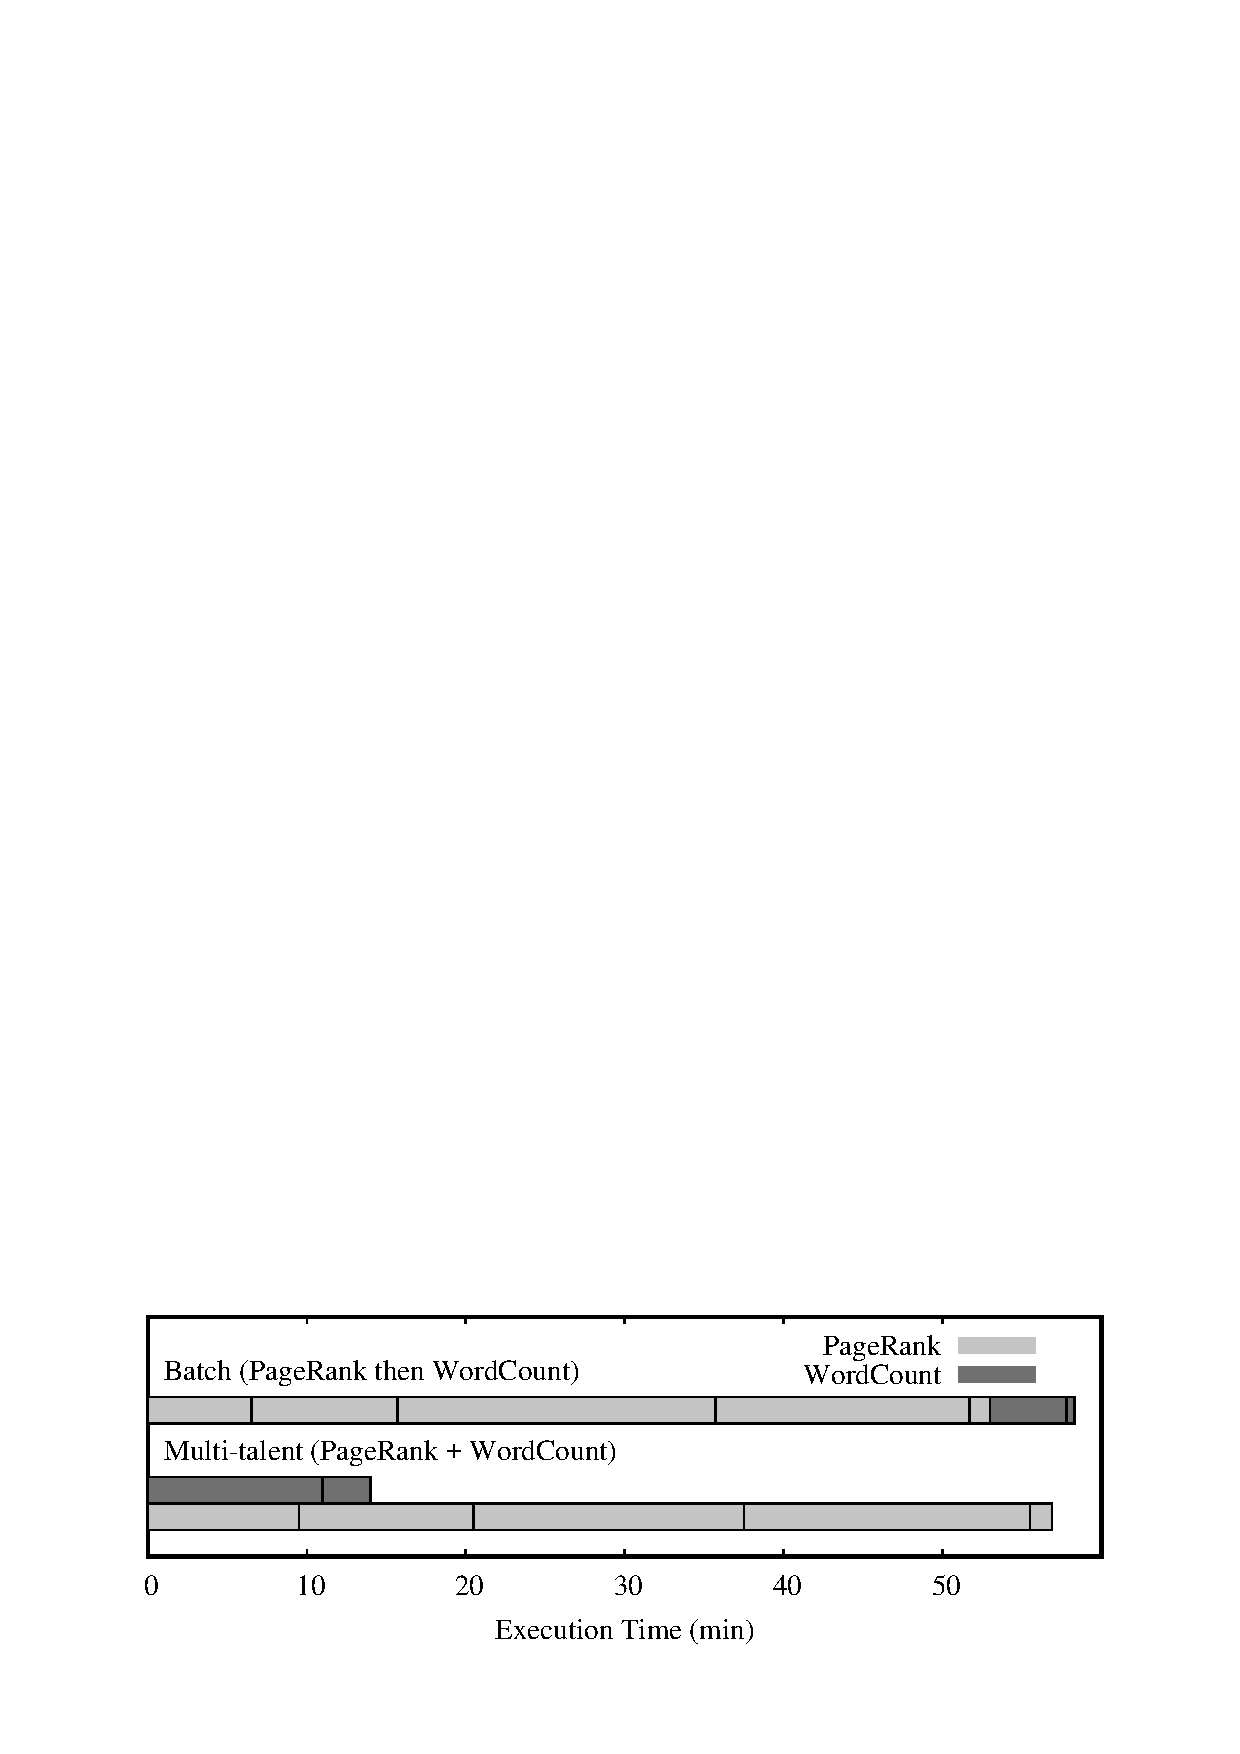
\includegraphics[width=0.45\textwidth]{memorypressure2.pdf}
\caption{Processing Batch and Mutli-tenant}
\label{fig:memorypressure2}
\end{figure}
\end{comment}

%No matter in batch processing or multi-tenant, different tasks can result in different memory pressure. Heavy memory pressure will lengthen the execution time of most tasks and decrease the throughout of jobs. The impact of memory pressure are more complex in multi-tenant in particular. Tasks with heavy memory pressure may benefit from these tasks with light memory pressure. But these tasks with light memory pressure must tolerate the memory pressure from other tasks.

%Although the framework provides several function APIs, these APIs both process the input data as key-value pairs: (key, value). All APIs process key-value pairs according to the key and user-defined functions. Some function APIs like \textit{map} just change the value; some function APIs like \textit{groupByKey} regroup values which have the same key; another function APIs like \textit{reduceByKey} aggregate values by the key. Thus, the result size of value is much different in different function APIs. For example, when one two-tuples is processed, existed key can result in the increase of value in \textit{groupByKey} but non variation in \textit{reduceByKey}. What's more, although different task implements the same function API, the result size in memory may be different because of the processing data type. Through the features of function APIs, we can classify the memory usage rate of function APIs to four type: \textbf{Constant}, \textbf{Sub-linear}, \textbf{Linear} and \textbf{Super-Linear}. After coarse-grained dividing the tasks implement function APIs to different types, when the memory pressure comes, these tasks lead to more memory pressure is clear.  

\section{Memory Usage Model in Tasks}

%// 模型的作用是什么没有说

%// 1,这些丰富的function API的特征是什么
%// 2,分类的原因
%// 3,通过实验证明有这四类的分类

%Some tasks use less memory to complete the work, while others cost much memory space as they produce massive long lived data objects. One of the major reasons is the function APIs in the processing pipeline. Although different frameworks provide different function APIs, they all have similar characteristics when measuring memory usage. We build models to describe the memory usage characteristics of a function API, and use memory usage rate to determine which model the task belongs to.

As discussed in previous section, some tasks consume less memory while some use much more memory as they produce massive long living data object, which are mainly generated by function APIs in the processing pipeline. Although there are various function APIs, some of them manifest a similar characteristic in terms of memory usage. Based on this observation, we build the models to capture the memory usage characteristic of a function API, and then the memory usage rate is used to determine which model the task belongs to.

%We find that we can build models to describe the memory usage characteristics of a task. Tasks in some models can produce less memory pressure than others because they use less memory to complete the work. One of the major reason is the function APIs in the processing pipeline. Although different frameworks provide different function APIs, they all have similar characteristics when measuring memory usage. We can use memory usage rate to determine to which model the function APIs belong.

\subsection{Memory usage models of APIs}

\begin{table*}[!t]
\small
\centering
\caption{Function APIs in Distributed Data Processing System} 
\begin{tabular}{ c | c | c | c | c | c | c }

\hline
\multirow{2}{*}{\textbf{Community}} & \multicolumn{2}{|c|}{ \multirow{2}{*}{\textbf{Core API} }} & \multirow{2}{*}{\textbf{Application Systems}} & \multicolumn{3}{|c}{\textbf{Partial Function APIs}} \\
\cline{5-7}
 & \multicolumn{2}{|c|}{} & & constant & sub-linear & linear \\
\hline
Hadoop & MapRedcue~\cite{vavilapalli2013apache} & Crunch & Pig, Hive, Yarn & map & reduce & \\
\hline
Microsoft & Drayd~\cite{isard2007dryad} & DryadLINQ & Scope, MadLINQ & map & reduce & join \\
\hline
Spark & \multicolumn{2}{|c|}{RDD~\cite{zaharia2012resilient}} & Spark SQL~\cite{armbrust2015spark}, GraphX~\cite{xin2013graphx} & map & reduceByKey & groupByKey \\
\hline
Flink & \multicolumn{2}{|c|}{Dataset~\cite{www:flink}} & Table~\cite{www:flink}, Gelly~\cite{www:gelly} & where & distinct & join \\
\hline
Google & MapReduce & FlumeJava~\cite{flumejava} & Tenzing, Pregel, Sibyl & parallelDo & combinValue & groupByKey \\
\hline

\hline
\end{tabular}
%\vspace{-2mm}
%\vspace{-4mm}
\label{table:apps}
\end{table*}

A data processing system provides several function APIs, which can be used to implement various applications. These function APIs take as input the input dataset and produce another dataset. The type of data in the dataset may be different. Table~\ref{table:apps} lists the function APIs provided by popular data processing systems. Most function APIs are sourced from MapReduce, a famous computing framework. Other function APIs are used to control the execution of jobs, the typical case of which is the shuffle operations. The shuffle operations are used between the \textit{Map} and the \textit{Reduce} phase, and are regarded as the separation point of a job, because the tasks after the shuffle operations (i.e., \textit{Reduce} tasks) need all results calculated by the tasks before the shuffle operations (\textit{Map} tasks).

These function APIs are all based on key-value pairs: (\textit{K}, \textit{V}). Some function APIs omit the parameter \textit{K} or \textit{V} for the convenience of users. Rather, the default value of the omitted parameters are used during the processes of \textit{map} or \textit{reduce}. The memory space is used by a function API to store the living data objects, because temporary data objects will be reclaimed by the garbage collection. The memory demand determines the characteristic of memory usage. Based on the key-value pairs, the memory size of living data objects is related to both \textit{K} and \textit{V} in the following ways.

\begin{itemize}

\item If the function API does not distinguish the parameter \textit{K}, it processes a record without involving other records. A record will produce a new record accordingly. If the new record is cached in memory, the consumed memory size will certainly increase. If the new record is processed as the input of the next function API or write-to-disk, it will be regarded as a temporary data object and quickly transmitted to the next function API. The size of temporary data object is ignored as it will be reclaimed in the next round of garbage collection.

\item If the function API distinguishes \textit{K}, it will involve all records to process these records with a particular \textit{K}. The function APIs that involve all records are usually called shuffle. While the shuffling stage processes the records to get all \textit{V} with a particular \textit{K}, two operations can be performed on \textit{V}: aggregation and non-aggregation.

\item If the function API does not aggregate the \textit{V}, it only puts \textit{V} in a collection without involving other \textit{V}. The collection contains the intermediate data and has a long lifetime because it is alive until the task processes all records. The collection is usually called the shuffle buffer. After a record is processed, the size of the collection increases by one element and thus the memory size of the shuffle buffer must increase.

\item If the function API aggregates the \textit{V}, the intermediate collection will be replaced by the aggregated value. We also call these data objects with long lifetime the shuffle buffer. Aggregation of \textit{V} means some operations will be performed on all \textit{V} with a particular \textit{K} and produce a new value. Thus, the resulting memory size of the collection will increase when \textit{K} has not appeared yet.

\end{itemize}

As the operations on \textit{K} and \textit{V} decide the size of the living data objects in memory, we build four models in this work to measure the memory usage of each function API when it processes a unit of data. The models are based on the size of the records that are processed, not on the number of the processed records, because the size of a record in each dataset is different. Memory usage refers to the memory space used to store the data objects with long lifetime except the garbage data objects. The four models are shown in Figure~\ref{fig:mur}. We determine the memory usage model of a function API by using the following lemmas.

\begin{figure}[!t]
\centering
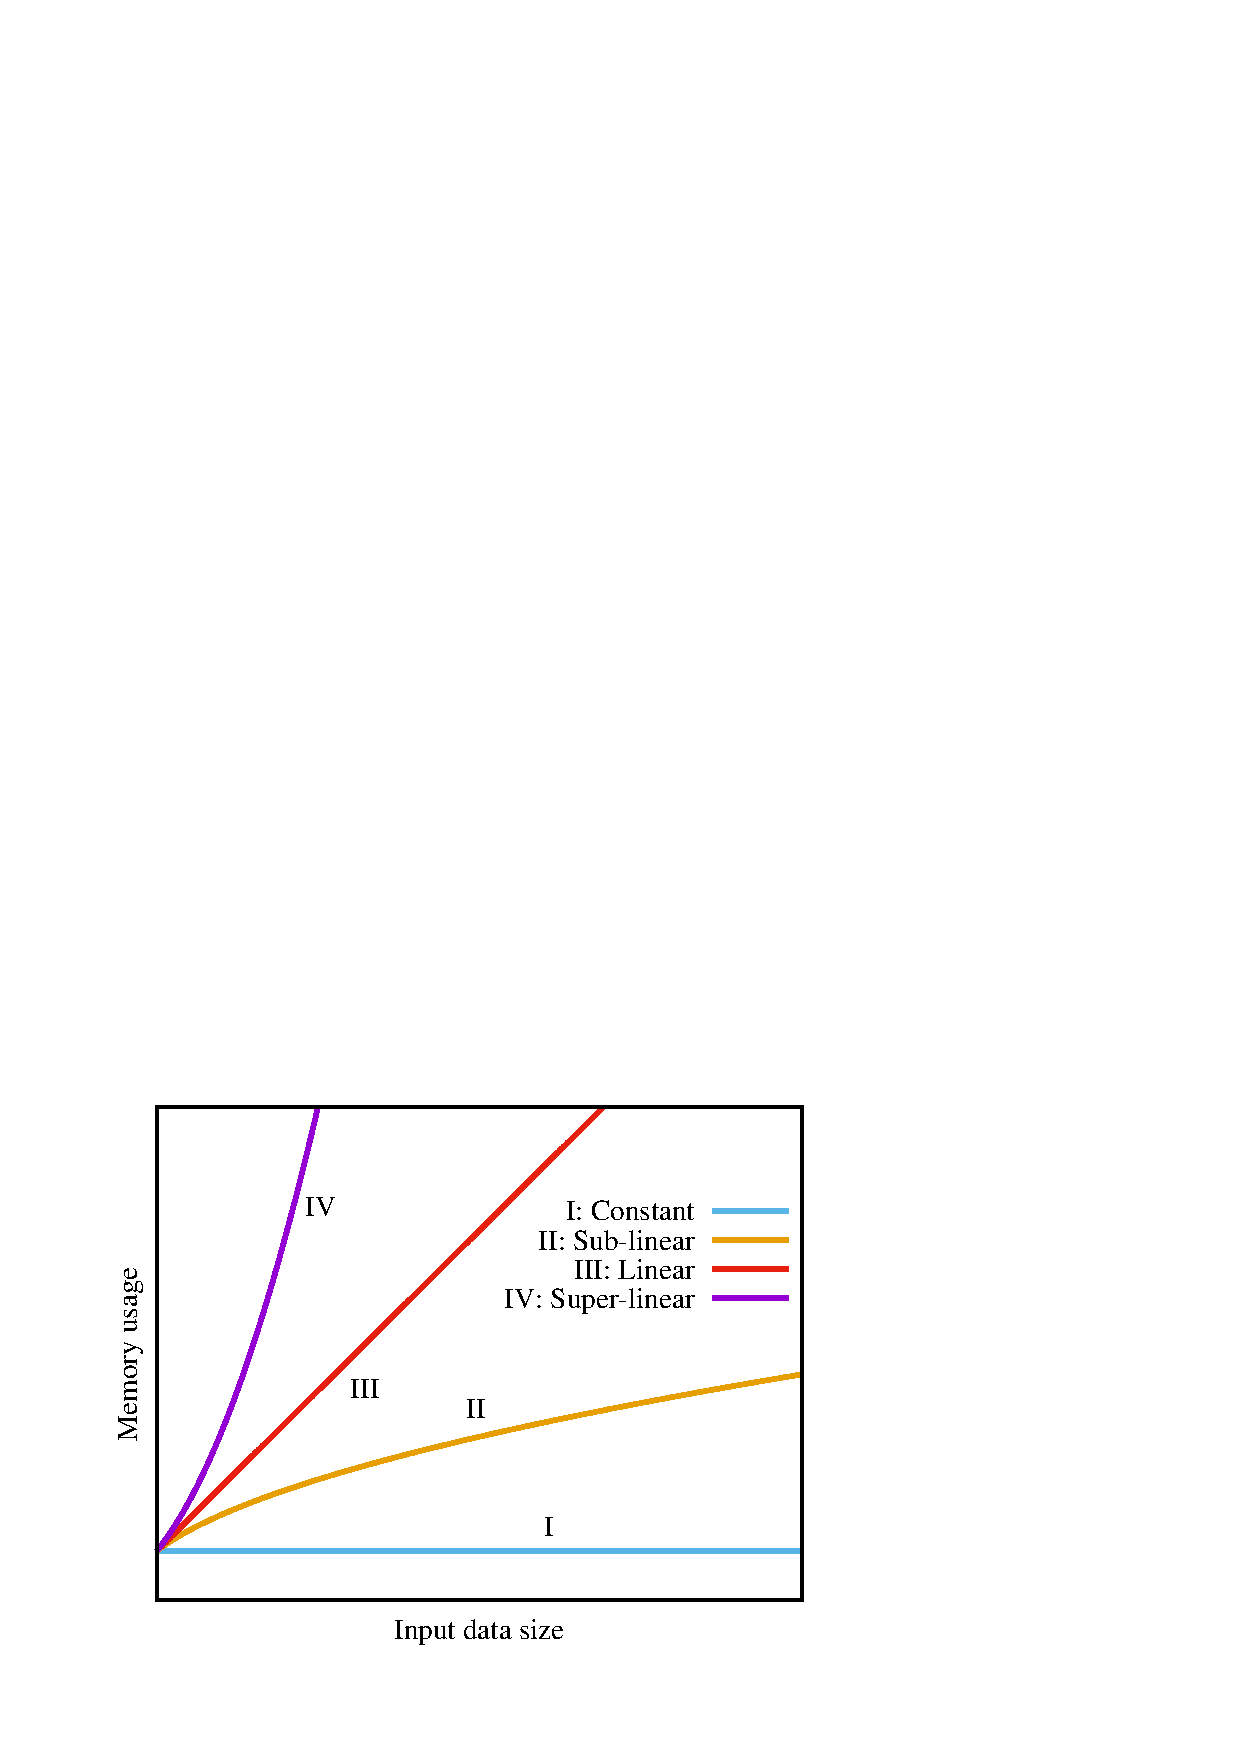
\includegraphics[width=0.3\textwidth]{mur.pdf}
%\vspace{-2mm}
\caption{Four coarse-grained models of function API}
%\vspace{-4mm}
\label{fig:mur}
\end{figure}

\newtheorem{lemma}{Lemma}
\begin{lemma}[Constant] The memory usage model can be defined as constant (Line I in Figure~\ref{fig:mur}) only when the following conditions are true:
\begin{enumerate}
\item The function API does not distinguish the key, \textit{K};
\item The resulting data will not be cached in memory.
\end{enumerate}
\end{lemma}

\begin{lemma}[Sub-Linear] The memory usage model can be defined as sub-linear (Line II in Figure~\ref{fig:mur}) only when the following conditions are true:
\begin{enumerate}
\item The function API distinguishes the key, \textit{K};
\item The function API aggregates the value, \textit{V};
\item \textit{K} appears randomly in the input dataset.
\end{enumerate}
\end{lemma}

Note that the reason why we require that \textit{K} appears randomly is because the size of intermediate data will increase only when the \textit{K} has appeared. If most \textit{K} gathers around some neighbouring records, the size of intermediate data will increase linearly.

\begin{lemma}[Linear] The memory usage model can be defined as linear (Line III in Figure~\ref{fig:mur}) when the following conditions hold:
\begin{enumerate}
\item The function API distinguishes \textit{K};
\item The function API does not aggregate \textit{V}.
\end{enumerate}
\end{lemma}

Both cache operations and the appearance pattern of \textit{K} affect the  size of intermediate data. Thus although some function APIs have the same operations on \textit{K} and \textit{V}, their memory usage models may be different. The constant model requires that intermediate data are not cached in memory. The increasing model is determined by the size of the cached data objects. The sub-linear model also requires the random appearance of \textit{K}. When a function API does not satisfy the above conditions, we need to redefine their models. In other words, the model is defined not only by the function APIs, but also by the user-defined function or data distribution. The memory usage model should be redefined when the following conditions are true:

\begin{itemize}

\item If the function API does not distinguish the \textit{K} and the result data are cached in memory, the speed of increasing size in memory can be 1) \textit{linear} (Line III in Figure~\ref{fig:mur}) when the function API does not work based on formal result; 2) \textit{super-linear} (Line IV in Figure~\ref{fig:mur}) when the function API produces larger result data, such as computing a histogram of the appeared numbers and all their divisors; 3) \textit{sub-linear} (Line II in Figure~\ref{fig:mur}) when the function API produces smaller result data along with the computation. 

\item If a function API i) distinguishes \textit{K}, ii) does not aggregate \textit{V}, iii) \textit{K} has not appeared yet in the input dataset or the appearance of \textit{K} is not random. The memory usage model of the function API should be linear.

\end{itemize}

Note that when function APIs belong to the same linear model, they can also be distinguished because the slope of the line in Figure~\ref{fig:mur} may be different. Steeper the slope is, the heavier impact the API function has on memory pressure. Based on the slope and four models, we can distinguish all function APIs in various data processing systems.

%If one function API does not satisfy one of the lemmas, we define them as the super-linear model. One possible super-linear model is shown as the Line IV in the figure. However, we find that no function API can be defined as the super-linear within the range of our research, most function APIs will show the memory usage as other three models in our evaluations.

%We should notice that the caching data and shuffle buffers are both long lifetime data objects in memory. Shuffle buffers are lived along with the shuffle operation. Some systems provide combine in map side which will effect the shuffle operation. When tasks need combine in map side, the function API will be executed in both map tasks (write) and reduce tasks (read). But when it needs not to combine, the function API will only be executed in reduce tasks, the map tasks will just produce the K-V pairs without any process. Other temporary data objects in function APIs will be reclaimed by garbage collection immediately.

%Some function APIs need both ensured \textit{K} and \textit{V}, such as \textit{shuffle}. According to the operations implemented on the \textit{V} with the same \textit{K}, these shuffle function APIs can be split to two groups: aggregate and non-aggregate. Aggregate operations are used to aggregate \textit{V} with the same \textit{K}. In this case, whether the result data in memory should increase the size is decided by the \textit{K}. But it's sure that non-aggregate operations must increase the size of result data in memory because no matter whether the \textit{K} has repeated emergence, \textit{V} is appended to the result data. What's more, besides the operations themselves affect the memory pressure, the type of \textit{V} also make some impact on the memory pressure. While the operations in running tasks are the same, we can also distinguish the influence on memory pressure by the data class they process.

%Some frameworks directly provide the \textit{cache} function API to cache the data in memory. This operation is different to other operations because it just applies for a memory space to store the dataset. JVM heap is usually the default region to store these data. Forward frameworks also provide storing off heap to save the execution memory space. No matter where the dataset store in, we just regard these memory pressure from JVM heap or system memory as unify.

%Most function APIs can satisfy these three items. Other function APIs, such as \textit{cache}, are designed to lengthen the lifetime of intermediate data but not influence the memory usage during processing. Further function APIs are also used to control the execution of jobs, the typical case is shuffle operations. Shuffle operations are used between Map and Reduce, and regarded as the break point of jobs. Because tasks after shuffle operations (reduce tasks) need all results of tasks before shuffle operations (Map tasks).  

\subsection{Memory usage models in tasks}
\label{subsec:taskmodel}

A task is implemented by at least one function API. Some systems define only one function API in each task, such as Hadoop. Other systems define the function APIs in a task according to the shuffle operations in the user-defined program, such as Spark and Dryad. As the shuffle operations are used to split the jobs, they implement both shuffle write and shuffle read. Thus, we consider the memory usage of a task in three phases: read, process, and write. The read and write phase of a task only contain one shuffle function API, or no function API if they read/write from/to disk or print in screen. If a task has a process phase, the phase contains several function APIs. 

The read and write phases of a task have independent memory usage models with a strict order. However, the memory usage model of the process phase is different. A function API in the process phase is always of the constant model. They never distinguish  \textit{K} and do not need to calculate all intermediate data. Thus they process each record as a temporary data object and quickly pass the intermediate data to the next function API. All constant models will not be shown in the memory usage of a task if the write phase of the task has the shuffle operations. This is because the size of the shuffle buffer is much bigger than the constant models. However, when the task caches intermediate data in memory, these intermediate data will be transmitted to the next function API after completing the current function API. Under this circumstance, the model is redefined. The redefined model will be combined with the independent models in a task. When there are several memory usage models in a task, we can only monitor the current memory usage model when we schedule the task. When reducing the current memory pressure, we use the current memory usage model to calculate the memory usage of the task.

Based on the memory usage models in a task, we only need the slope of each line in Figure~\ref{fig:mur} to determine the current memory usage model. We term the slope the \textit{memory usage rate}. Thus, the memory usage rate of a task is defined as the memory size of the newly produced long-living data objects when a task processes a unit of input data.

%It is clear that when the function API distinguishes the \textit{K} and not aggregates the \textit{V}, the memory usage of result data will increase after each record is processed. Thus it will have stable necessary of memory space compared to sub-linear model. The linear model can be defined as the Line III in Figure~\ref{fig:mur}. We notice that as the slope of line can be different, linear model can also have different impact on the memory pressure. The slope can be decided by the type of result data.

%Some special tasks will be redefined as linear too. The first one is when tasks cache data in memory. When the result data of constant model is cached in memory, the memory usage will increase undisputed. However, it is not applicative for sub-linear type because the result data has already stay in memory with long lifetime. The second one is the appearance of \textit{K} when some function APIs distinguish \textit{K}. When the appearance of \textit{K} is not balanced, the memory usage will also increase after processing one record. Thus these function APIs will also be redefined as linear.

%Function APIs are transparent to tasks and running discrepant with different dataset, and it's not sensible to clearly distinguish which function API the task executes. Although, we can coarse-grained distinguish these function APIs along with the input dataset features. Memory usage rate of a task combines the features of both function API and input dataset: i) different operations result in different growth pattern of middle data in memory, which means the influence on memory pressure; ii) the data class of input dataset decides the size of each record (key-value pairs as usual) in memory. 


%If function APIs in one task cannot satisfy any of the lemmas, we define them as the super-linear. One possible memory usage model of super-linear is shown as Line IV in Figure~\ref{fig:mur}. super-linear type is rare in current data processing systems. Anyhow we build this model to cover these complex function APIs.

%\textbf{Constant} Simple function APIs that come from \textit{map} are both constant model, such as \textit{map}, \textit{flatMap}. These function APIs process one record and result in another record. Thus the result data in memory is ensure. We should notice that most result data processed by these function APIs will not be stored directly in the memory, they have three different directions: i) used in next function API. The function APIs with constant model in this scene just produce the middle result for next function, thus these data in memory are all temporary variables which just occupy a constant space. ii) saved to disk. The data produced will be directly write to file stream, thus a constant memory space are occupied also. iii) saved to memory. This scene does not accord with the constant type, because each result data is saved in memory and the occupied space are linearly growth.  

%\textbf{Sub-linear} Most aggregate function APIs can be sub-linear, such as \textit{reduceByKey} and \textit{reduce}. The root of sub-linear is the repeatability of \textit{K}. When the aggregate function APIs aggregate \textit{V}, if \textit{K} has existed the result \textit{V} will just be update, thus the occupied space remain unchanged; if \textit{K} is new and a new record will be append to the result data, the occupied space will increase. However, this coarse-grained model is based on the equally distributed \textit{K}. We can just weak this type to linear type if the layout of K not satisfies this rule, although this type has less memory usage than linear type.

%\textbf{Linear} Non-aggregate function APIs are the most directly type because it's clear that when processing one record the result data in memory must increase its size, such as \textit{groupByKey} and \textit{join}. No matter whether \textit{K} has existed, \textit{V} will be append to the data object with the same \textit{K} in result data. Although  most tasks with non-aggregate function APIs or weak sub-linear type are regarded as linear type, we can still distinguish these tasks by the slope. The slope of the linear are decided by the result data class. Complex data class will occupy more memory space than simple data class, which means the slope of the linear in memory usage are larger. The larger slope in memory usage rate is considered to lead to more memory pressure compared to tasks with low slope in memory usage rate.

%\textbf{Super-linear} Super-linear type is rare in current data processing systems. A typical function API is \textit{flatMap} which flats the record (the data class of record should be collection) to records one by one. Although flatMap provides the flatten operation, if the map operation inside doesn't extend the size of each record, the memory usage rate type of this task is also linear or constant. Anyhow we build this type to cover these complex function APIs with super linear memory usage rate. 

%After the coarse-grained type of all running tasks are ensured, we can coarsely distinguish which task can lead to more memory pressure when we consider the memory usage rate. Based on the coarse-grained model, we can apply for memory usage rate based scheduler to mitigate the memory pressure.


\section{Design of MURS}
\label{sec:desgin}

Memory pressure essentially describes the usage of heap in managed languages. We first compute the heavy tasks which may have linear or super-linear model, or have large input dataset. The fundamental scheduling mechanism is suspending these heavy tasks as memory pressure occurs, and then resuming the suspended task when memory pressure recedes or light task completes.

%\subsection{Memory management}

%// 这一段的目的不够明确

%Although the memory usage rate describes the memory usage features about different tasks, we should also separate the memory management of the data processing system itself and JVM. Because the data processing systems always take some measures to avoid the out of memory error by spilling data to disk which based on the memory management themselves. When the spill occurs, the memory may suffer pressures although we stop tasks.

%Most data processing systems split the allocated memory to cache memory and execution memory. The cache memory is only used to store data with long lifetime. While execution memory is only used for temporary or middle data, such as shuffle result that will be write to disk. Cache memory and execution memory can be managed uniformly. What's more, these execution memory are allocated to each task independently. These make up the memory management of data processing system and also decide the memory usage rate of one task based the function API. When considering about the memory pressure, it's conflict to consider the memory management of data processing system. Because after one task is completed, the allocated execution memory will be reclaimed but the data objects are also in JVM heap. On another hand, some tasks will not only use the execution memory but also cache memory. Thus, in order to measure the memory pressure, we just consider the usage of JVM heap but not the memory management of data processing system.

%In the memory management of JVM, the heap space is split to young generation, old generation and other generations. The pinch of young generation leads to \textit{Minor GC}. Minor GC will move the lived data objects from young generation to old generation. The pinch of old generation leads to Full GC. If most long lifetime data objects remain in the old generation, frequent full gc will occur and lead to bad performance. Some garbage collection algorithms are working only in young generation or old generation, and some can works on both generations. In any case, the garbage collection is triggered when the used space of heap get the threshold.

Firstly, we define the memory pressure as follows: when the proportion of used heap has reached the threshold value. The threshold is set according to the trigger of garbage collection. In addition, we set two thresholds here. The first threshold, called as yellow value, is used to indicate the memory pressure. When the percentage of long lived data objects in the heap meets the yellow value, it means frequent full GC will occur. Full GC means that the garbage collector will clean all the heap, and it is usually expensive. Another threshold value, called as red value, is used to avoid spilling. The red value shows the pressure under which the out-of-memory error will occur or some data will be spilled to disk. The default values of yellow and red are 0.4 and 0.8, based on our evaluation. It is proposed that, if the memory pressure is heavy, we should reduce the value.

With the yellow and red value, an accurate percentage of long lived data objects in the heap actually determines the efficiency of threshold. As JVM splits the heap to young generation and old generation, minor GC cleans the young generation and moves alive data objects to the old generation. Thus the percentage of heap usage after a minor GC describes the lived data objects in the heap. After each full GC, dead data objects in old generation will also be reclaimed, we revise the percentage of long lived data objects in the heap according to the current percentage of heap usage.

%With the yellow value and red value, the percentage of data objects with long lifetime in the heap are actually important. As we know, garbage collection algorithm is based on mark-clean; thus, long-lived data objects in the heap will lead to expensive marking and cleaning costs. What’s more, long-lived data objects directly result in frequent full garbage collection. In order to get the percent of long lifetime data objects in heap, we set it to the size after a minor GC, which just cleans parts of the heap quickly. These data objects are lived in the heap, and most will also be lived along with the tasks.  

%Although the scheduler wishes to reclaim as many data objects as possible, the space reclaimed the last time will have an error with the expected reclaimed space. The error actually means the space occupied by these data objects was stored in an old generation and reclaimed before the task completed. We count the error and consider it in the last computation. Because tasks themselves work with the iterator, the produced data objects have steady regulars.

\IncMargin{0.4em}
\SetAlFnt{\small}
\begin{algorithm}[!t]
%\DontPrintSemicolon

\SetKwInOut{Input}{Input}\SetKwInOut{Output}{Output}
\SetKwProg{Fn}{Function}{}{end}
\SetKwFunction{CST}{ComputeSuspendTasks}
\SetKwFunction{CS}{ComputeSpill}
\SetKwData{F}{\small{final}}

\Input{Array of running tasks $R$\;}
\Output{Array of suspended tasks $S$\;}
get the Memory Usage Sampler $Sampler$\;
get the Memory Manger $SM$ of System\;
get the Memory Manger $JM$ of JVM\;
get the queue including suspended tasks $SQ$\;
\lIf{Usage of $JM$ is lower than the yellow value}{return}
\lElseIf{Usage of $JM$ is lower than the red value}{\CS}
\lElseIf{$SQ$ is not empty}{return}
\lElse{\CST}

\BlankLine
\Fn{\CST}{
  $freeMemory \leftarrow JM.freeMemory$\;
  $consumption[] \leftarrow SM.tasksMemoryConsumption$\;
  $rate[] \leftarrow Sampler.getMemoryUsageRate$\;
  $percent[] \leftarrow Sampler.getCompletePercent$\;
  $S \leftarrow R$\;
  \While{$freeMemory > 0$}{
    $minRateTaskId \leftarrow reate[].min$\;   
    \lIf{\CS}{reduce the running cores and return}
    $memoryNecessary \leftarrow comsumption[taskId] * (1-percent[taskId])$\;
    $freeMemory -= memoryNecessary$ \;
    $S$ remove minRateTaskId \;
    push minRateTaskId to $SQ$\;
    $rate[]$ remove minRateTaskId \;
  }
  \KwRet{$S$}
}
\BlankLine
\Fn{\CS}{
  $taskId \leftarrow$ task Id \;
  $totalMemory \leftarrow JM.totalMemory$ \;
  \lIf{$comsumption[taskId] > totalMemory / R.length$}{\KwRet{True}}
  \Else{
      $memoryNecessary \leftarrow comsumption[taskId] / percent[taskId]$\;
      \lIf{$memoryNecessary > totalMemory / R.length$}{\KwRet{True}}
      \lElse{\KwRet{False}}
      }
}
\caption{Scheduling mechanism on JVM}
%\vspace{-4mm}  
\label{code:scheduler}
\end{algorithm}

These indicators of memory pressure are the infrastructure of the memory usage rate based scheduler. The scheduler is designed in Algorithm~\ref{code:scheduler}. The input is the current running tasks and the output is the proposed suspended tasks. Some basic managers should be accessible to record the indicators of memory pressure. We design a \textit{Sampler} to record the real-time metrics of current running tasks. Sampler runs seasonally to update the metrics of each task and compute the current memory usage rate, such as the size of input dataset, the number of processed records, and the size of result data.

If the memory pressure is light, or the system already has suspended tasks, we directly return without propose (lines 4, 6). If the memory pressure has reached the red value, MURS will avoid spilling (line 5). When the memory usage of JVM heap touches the yellow value, we get the memory usage rates of all running tasks from the sampler and other details of current memory (lines 9-12). We take the measures to process current running tasks step by step in the following order: constant, sub-linear, linear, and super-linear. Free memory subtracts the necessary memory of the currently processing task every time. When free memory is not enough for the remaining unprocessed tasks, scheduler will stop processing tasks (lines 14-20). This method is able to distinguish these tasks with sub-linear model but working as heavy tasks if they process larger dataset, or tasks with super-linear model but working as light tasks if they consume less memory space. Processed tasks are removed and the remained tasks will be returned. The returned tasks are heavy tasks and will be set to suspend. In order to avoid potential starvation, suspended tasks are pushed to a queue (line 21). FIFO algorithm allows us to resume the first suspended task to avoid starvation. 

MURS suspends the proposed heavy tasks to prevent memory pressure increasing at a high rate of speed. Note that if all running tasks are heavy tasks, MURS still schedule tasks with the same algorithm. It always chooses these tasks have relatively small memory usage rate in total tasks. 

Function \textit{ComputeSpill} is designed to avoid spilling. As the running tasks share the JVM heap together, the maximally allocated space for each task is ensured to less than $1/N$ while $N$ is the number of running threads. When the consumption exceeds the maximal space, the spill or out-of-memory error will occur. Running tasks that satisfy the \textit{ComputeSpill} (lines 27, 30) are also suspended to decrease the parallelism in order to acquire enough memory space after memory pressure goes away.   

When a running task completes, we resume a suspended task popped from the queue accordingly. After the memory pressure recedes, meaning the usage of JVM heap is below the yellow value after a full GC, the remaining suspended tasks will also be removed. However, one completed task only resumes one suspended task and the memory usage below yellow value will remove all suspended tasks.

\begin{comment}
\subsection{Multi-launch with MURS}

When light tasks have a large proportion in the running tasks, or memory space is enough for total running tasks, the memory pressure is light. Light memory pressure usually means that memory space will suffer less allocation and reclamation. However, properly increase the frequency of memory allocation and reclamation can improve the efficiency of memory usage. With hyper-threading technology, we can increase the parallelism of submitted jobs as well as memory pressure. Fortunately, MURS releases our scruple that memory pressure increases seriously with high parallelism. Thus, we propose multi-launch to improve the efficiency of memory usage with MURS.

Multi-launch works when tasks are launched to workers. Multiple tasks are launched to workers compared to the original configuration. If the configuration has remained free CPUs in the workers, multi-launch will work better because an extra task can execute more quickly on a physical CPU than on a logic CPU. The multiple should not be too large, because 1) maximally accessible memory space in heap is limited; 2) the interprocessor communication time can not be ignored; 3) I/O parallelism is limited by disk.

\end{comment}








\begin{comment}
\subsection{Balance of the Stop}

When the heavy tasks are suspended, they will suffer from a long wait. A long wait will result in two problems: 1) CPU resource is waste during suspending tasks; and 2) stopped tasks can be stragglers. 

Although the tasks with linear memory usage model will lead to more memory pressure, frequent stopping is not tolerated in these tasks. And it is a little regretful to waste CPUs when some tasks are suspended. Multi-launch is designed to enhance the fairness:

\begin{enumerate}

\item When tasks are allocated to workers, multiple tasks will be launched. This will result in memory pressure at express speed.

\item After the mitigation of MURS, tasks with a constant or sub-linear memory usage rate will complete and memory pressure will recede. Thus, the tasks with a linear memory usage model will run smoothly with light memory pressure and more resources (both core and memory).

\end{enumerate}

However, multi-launch is not always advised. When the space of execution memory is much smaller or spill is accessed, multi-launch will affect the memory pressure to a great extent. Although our scheduler can prevent the increasing speed of memory pressure, much higher parallelism will decrease the available heap space of one task. Less max available space of one task will result in out of memory error.

As we know, stragglers are common in current distributed data processing systems. Many reasons, such as the heterogeneous environment~\cite{matei:heter}, can lead to one task taking much more time than other tasks and affects the completion of a job. Our scheduler even stops some tasks to prevent the execution. In fact, if the heterogeneous environment is gotten rid of, the cost of computation itself is much more stable. However, garbage collections can prominently increase the execution time of tasks, especially in current in-memory data processing systems, as shown in Figure~\ref{fig:memorypressure}. Our scheduler can control heavy memory pressure, based on the memory usage rate. With low memory pressure, these tasks can be free from the stop-the-world of garbage collection by waiting for constant or sub-linear tasks, and fortunately, the constant or sub-linear tasks can execute quickly with less memory pressure. Thus, we take some time to wait, but free more pressures of garbage collection. 
\end{comment}

\section{Implementation}

We implement MURS in Spark 1.6.0 with approximately 1000 Scala codes. MURS contains a scheduler and a sampler. The scheduler implements the Algorithm~\ref{code:scheduler}. The sampler runs seasonally to update the metrics related to the current running tasks, Spark memory manger and JVM heap manager. Each executor launches one scheduler and one sampler in Spark.

The sampler works seasonally to collect and compute all metrics in the scheduler. It is implemented in the original task scheduler because all tasks in Spark are accessible in the scheduler. The sampler updates the following metrics in a task after a record is processed:

\begin{enumerate}

\item Read phase. Only the shuffle buffer in the shuffle read phase results in memory pressure. Thus the sampler updates the metrics in shuffle reader. The updated metrics include the number of processed records, the number of total records, the size of total records and the size of the shuffle buffer.

\item Process phase. During the process phase, only the operation of caching data produces the memory pressure. Thus the sampler updates the metrics in {\ttfamily \small CacheManager}. {\ttfamily \small CacheManager} is invoked by the function APIs to unroll the intermediate data in memory. The updated metric is the size of cached data objects unrolled by this task.

\item Write phase. Since only the shuffle buffer in the write phase causes memory pressure, the sampler updates metrics in the shuffle writer. The updated metrics are the size of the shuffle buffer, the number of write records, and the number of total records. 

\end{enumerate}

The sampler also updates some metrics of the memory mangers, including the current memory usage of a task, free memory space, and the current proportion of used heap. Based on these metrics, current memory usage rate of a task is computed as the quotient of two increments: $\bigtriangleup size_{used\_memory} / \bigtriangleup size_{processed\_records}$. All computed values of the memory usage rate are stored in a buffer. The changing trend of the memory usage rate determines the model that the task belongs to.

%The sampler works as a manager to collect and compute all data from current running tasks. The sampler is realized as a field of \textit{TaskScheduler} in Spark. There are two types of tasks in Spark: \textit{ShuffleMapTask} and \textit{ResultTask}. \textit{ShuffleMapTask} will write shuffle data to disk, which will result in heavy memory pressure. \textit{ResultTask} will return the data to driver with light memory pressure. Both of them implement the \textit{TaskMemoryManager} in Spark to update the real-time memory usage. These tasks share the only task scheduler, thus the sampler can collect data from all the running tasks. As these tasks process data as iterator, sampler updates the used memory size of one task from \textit{TaskMemoryManager} and the number of processed records each time. The size of processed data can be computed by the processed records, total size, and total records. And the memory usage rate means the quotients of increased used memory size and processed data size.

%{\ttfamily \small CacheManager} manages the caching data in Spark. When tasks need cache data, they invoke {\ttfamily \small CacheManager} to roll the data that result in memory pressure. If the input of a task is from {\ttfamily \small CacheManager} or disk, the task has no read phase. After reading one record, the record can be transmitted to next function API quickly.

%\textit{CacheManager} manages the caching data in Spark. When tasks need cache data, they invoke cache manager to roll the data that result in memory pressure. Reading from cache manager is different from reading from disk. As the data has already been stored in memory, we cannot consider the memory pressure of reader. Thus, the caching data in tasks will be computed in the memory usage rate during writing but not reading.

The scheduler detects the total memory usage from the sampler seasonally. When it reaches the yellow value in Algorithm~\ref{code:scheduler}, scheduler proposes the suspended tasks. All tasks process data in {\ttfamily \small InterruptibleIterator}, which can be interrupted by the system or scheduler. We build a flag to suspend the {\ttfamily \small InterruptibleIterator}. After MURS proposes suspended tasks, we update the flag of each task in task scheduler. If the flag is true, the {\ttfamily \small InterruptibleIterator} will suspend itself and the task is also suspended. When MURS resumes the task, it only needs to set the flag of this task to be false.

%The scheduler detects the total memory usage in JVM seasonally. When it reaches the yellow value in Algorithm~\ref{code:scheduler}, it proposes the stopping tasks. The proposal will be used to update the flag of each task in task scheduler. Both \textit{ShuffleMapTask} and \textit{ResultTask} process data in \textit{InterruptibleIterator}. We put the flag in this iterator. The flag is updated by the task scheduler each time the scheduler gives new proposals. When the flag is true, the \textit{InterruptibleIterator} will stop itself and the task also stops working.

When we consider the Spark as a server, we choose Spark Job Server 0.6.2~\cite{www:jobserver}. Each job in Spark works within the only {\ttfamily \small SparkContext}. Spark Job Server first defines the shared context. We set the scheduler mode as FAIR and build a scheduler pool in the context. The scheduler mode means the processing sequences when jobs come from multi-tenant. Fair scheduler will process tasks from each job fairly. All jobs are submitted to Spark Job Server instead of Spark. Spark Job Server will resubmit the job to the shared context in Spark. Thus, all jobs are processed in one context in Spark.
\section{Evaluation}

\subsection{Configuration}

We use four nodes as workers and one node as the master in the experiments. Each node has two eight-core Xeon-2670 CPUs and 64GB memory. The file system is mount on one SAS disk, running RedHat Enterprise Linux 5 (kernel 2.6.18). The JDK version is 1.7.0 for Spark 1.6 and Spark Job Server 0.6.2. We count not only the execution time of each application, but also the details of runtime situations.

\begin{table}[!t]
\small
\centering
\caption{Function APIs in each Application}
\begin{tabular}{ c | c | c | c }

\hline
\textbf{App} & \textbf{Stages} & \textbf{Function API(s)} & \textbf{Cache} \\
\hline
Grep & 1 & \textit{filter} & No \\
\hline
WC & 2 & \textit{flatMap} \& \textit{reduceByKey} & No \\
\hline
Sort & 3 & \textit{distinct} \& \textit{sortByKey} & No \\
\hline
PR & N & \textit{groupByKey} \& \textit{map} \& \textit{reduceByKey} & Yes \\
\hline

\hline
\end{tabular}
%\vspace{1mm} 
%\vspace{-8mm}
\label{table:app}
\end{table} 

We choose four typical benchmark applications in Spark to evaluate the performance: Grep, Sort, WordCount(WC), and PangeRank(PR). Grep has only one stage: it filters the records that do not satisfy the conditions. WC has two stages: it counts the number of each key in the input file. Sort has three stages: it sorts all records by key in the input file. While PR is a typical iterative computations, and one of its most important features is that it will cache data in memory. We choose these four benchmarks because these applications contains different function APIs, as shown in Table~\ref{table:app}. For Sort  and WC, the datasets are produced by HiBench Random Writer with 1B unique key numbers. The size of input dataset is 30GB in Sort, and 50GB in WC. For Grep and PR, we use the real graphs: webbase-2001 (30GB)~\cite{boldi:webgraph} to evaluate the performance of MURS. Key-value pairs of each record in all input dataset have the similar size. We tun the size of heap size to evaluate different memory pressure. Garbage collection time is used to measure the memory pressure. These applications are grouped to evaluate different scenes and submitted to Spark Job Server together.

\subsection{Memory pressure without caching}

Most current data processing systems are designed based on MapReduce, but only parts of them provide the in-memory computing model that caches data in memory to speed up the system. Thus, we first evaluate these applications without caching data in memory to stand for common frameworks working with key-value pairs, such as Hadoop and Hive.

We choose three applications: Sort, WC, and Grep. These applications have no caching operation. Each application has similar implementation in MapReduce. Grep reads data from disk and filter these records which satisfy the given conditions. Most data objects are temporary. Shuffle buffers in Sort and WC are data objects with long lifetime. Thus tasks in Sort and WC are clear to heavy tasks in MURS. The results of each submission are shown in Figure~\ref{fig:pressurewithoutcache}. The best improvement of MURS can be 1.8x to 2.9x compared to Spark in each evaluation. The reduction of garbage collection contributes to most improvement.

\begin{figure*}[!t]
\centering
\subfigure[Sort+Grep]{
\label{fig:subfig:sort-grep}
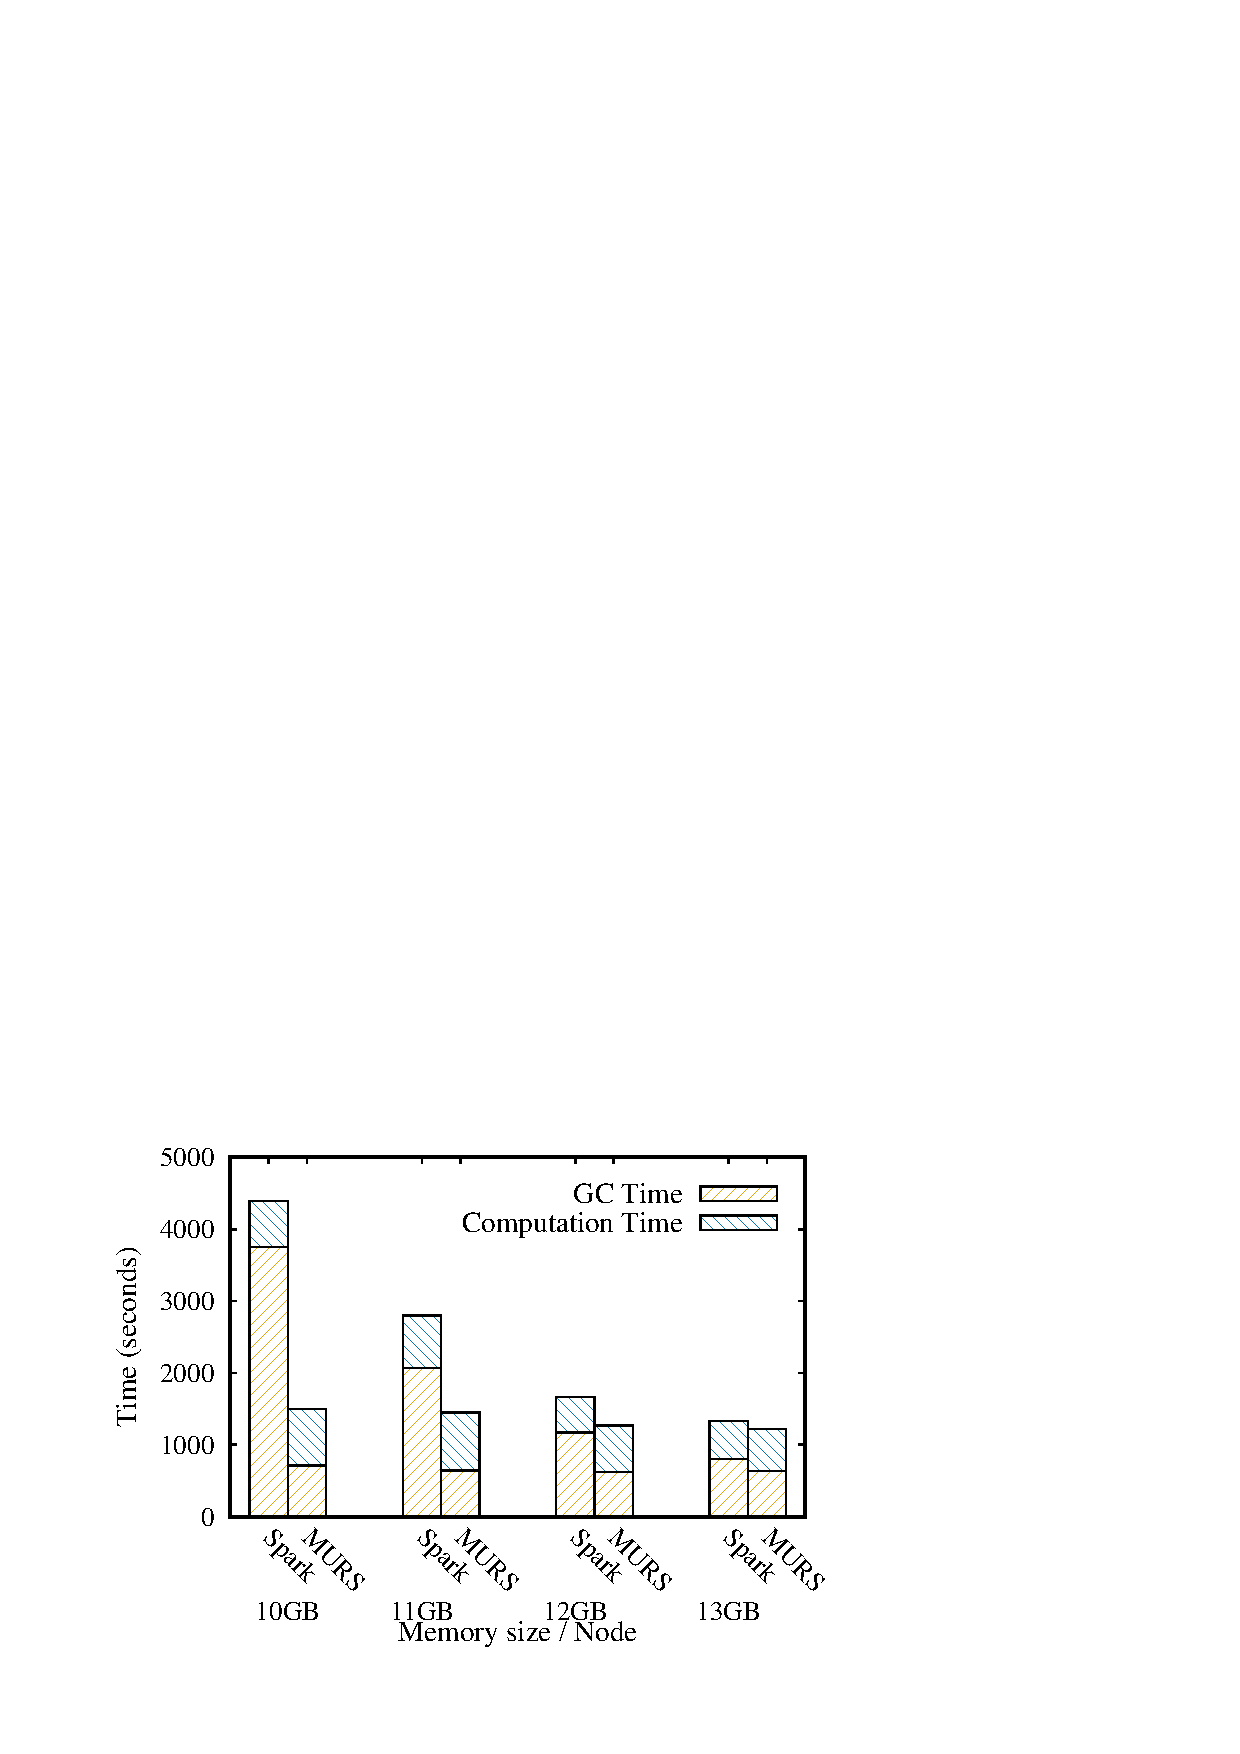
\includegraphics[width=0.3\textwidth]{sort-grep.pdf}}
%\hspace{-3ex}
\subfigure[WC+Grep]{
\label{fig:subfig:wc-grep}
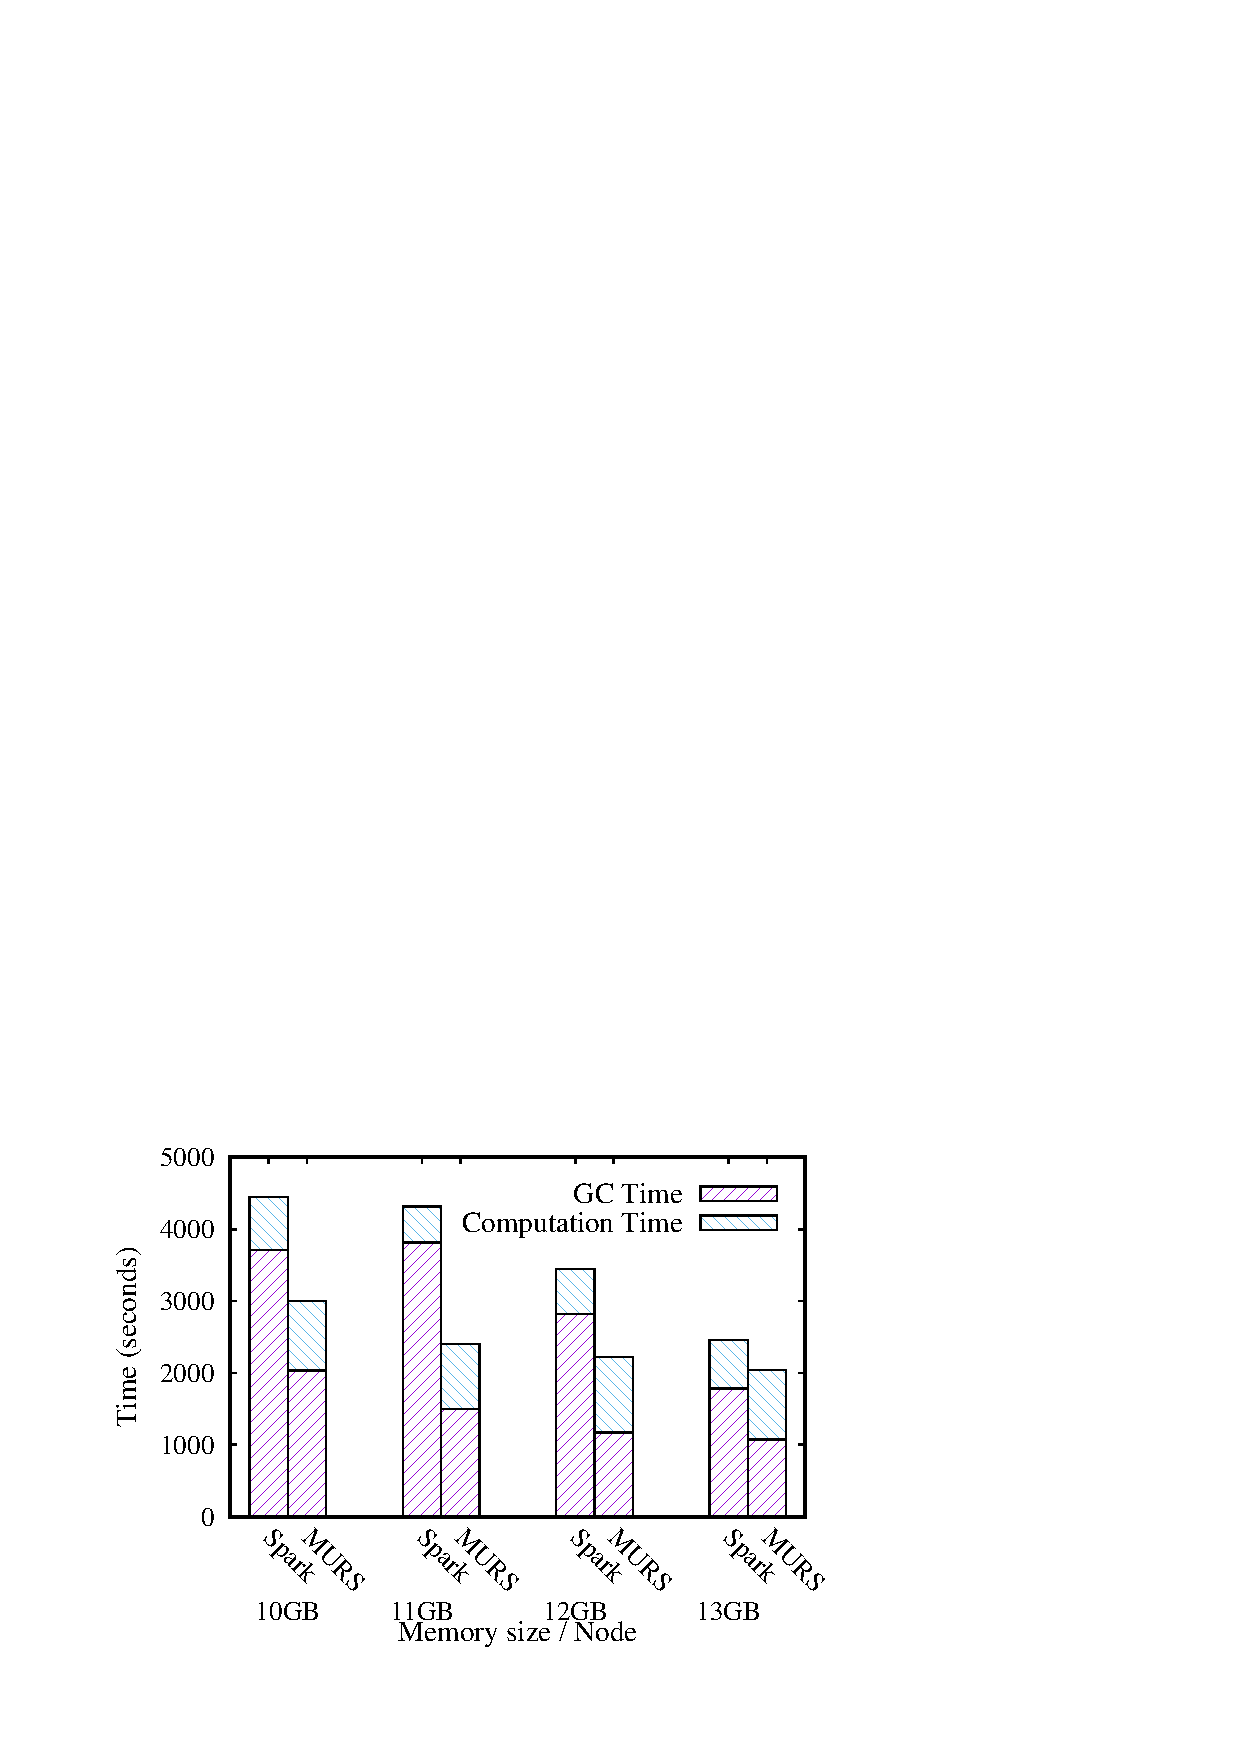
\includegraphics[width=0.3\textwidth]{wc-grep.pdf}}
%\hspace{-1.9ex}
\subfigure[Sort+WC+Grep]{
\label{fig:subfig:sort-wc-grep}
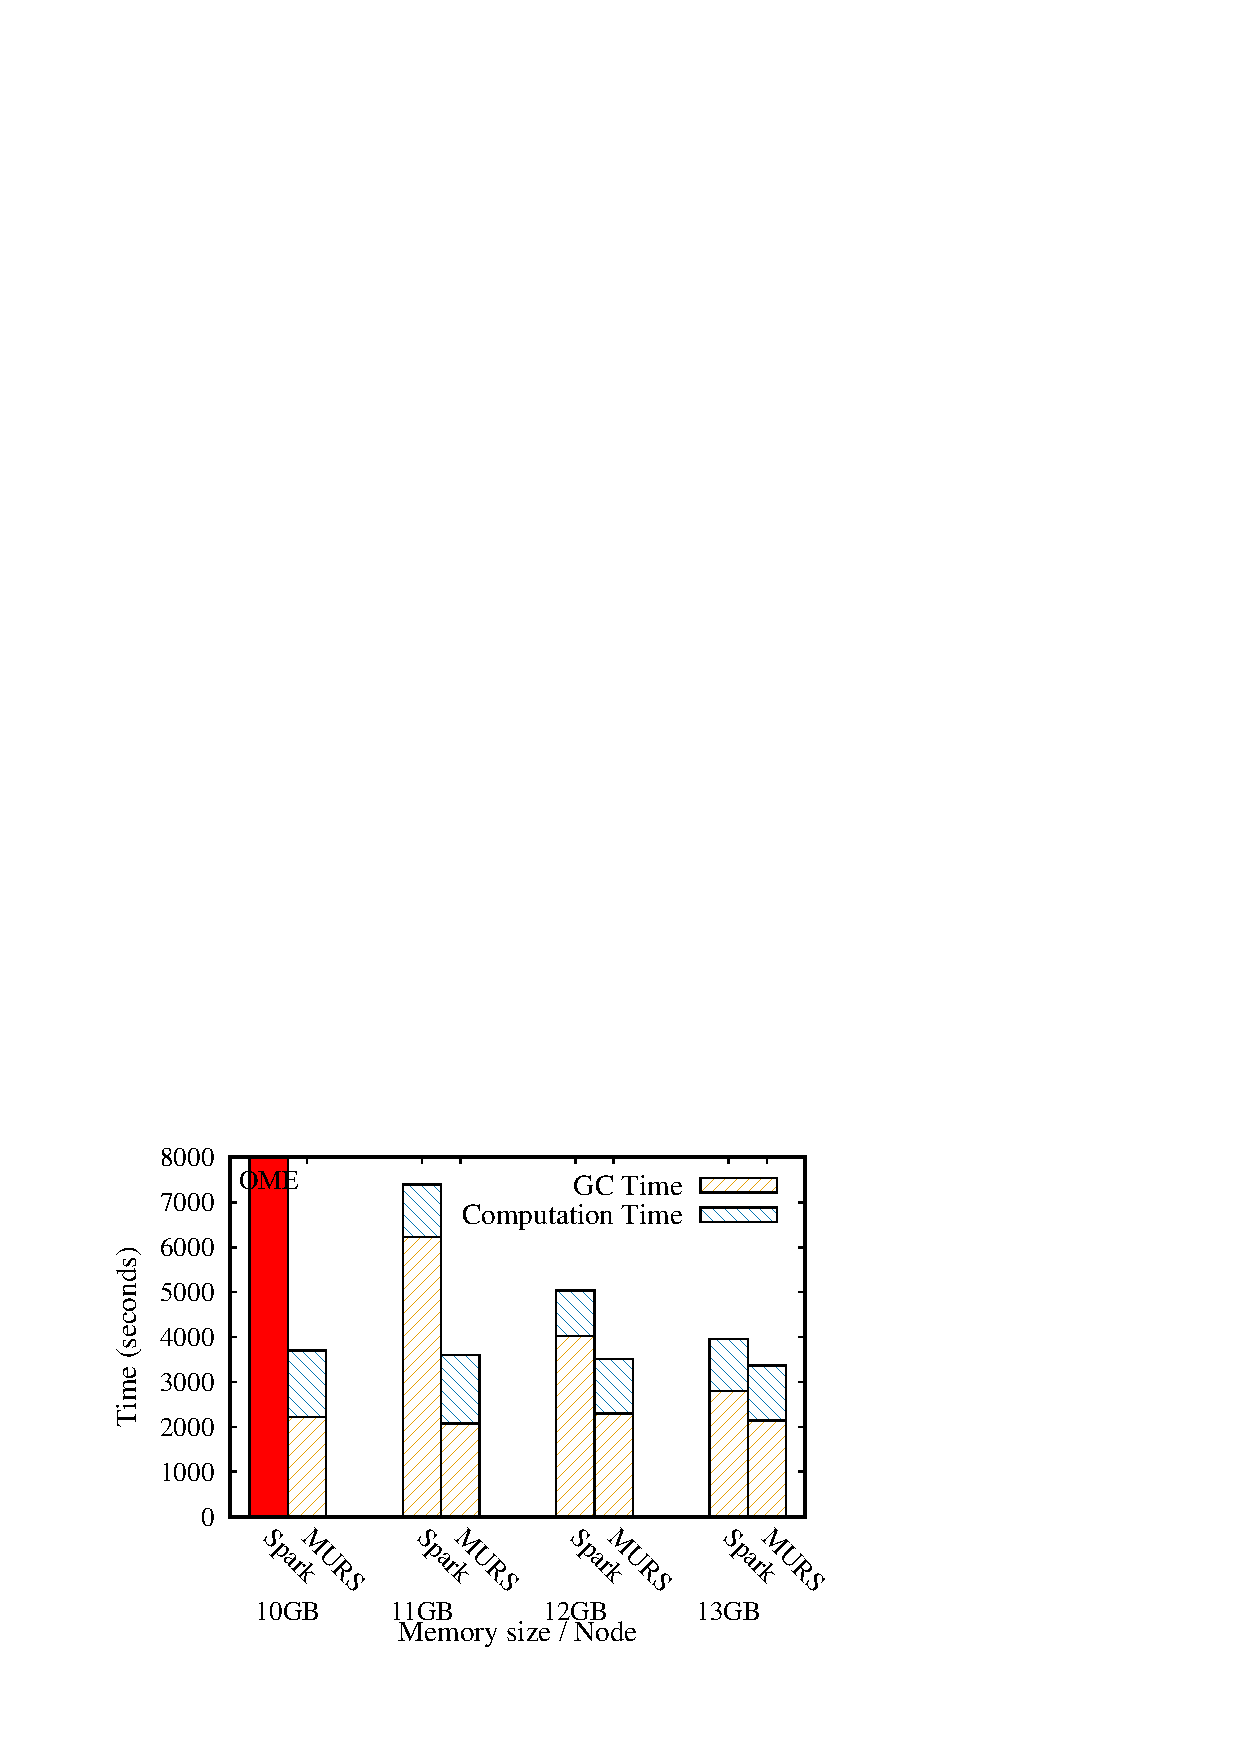
\includegraphics[width=0.3\textwidth]{sort-wc-grep.pdf}}
%\hspace{-1.9ex}
%\subfigure[Active tasks]{
%\label{fig:subfig:activetasks}
%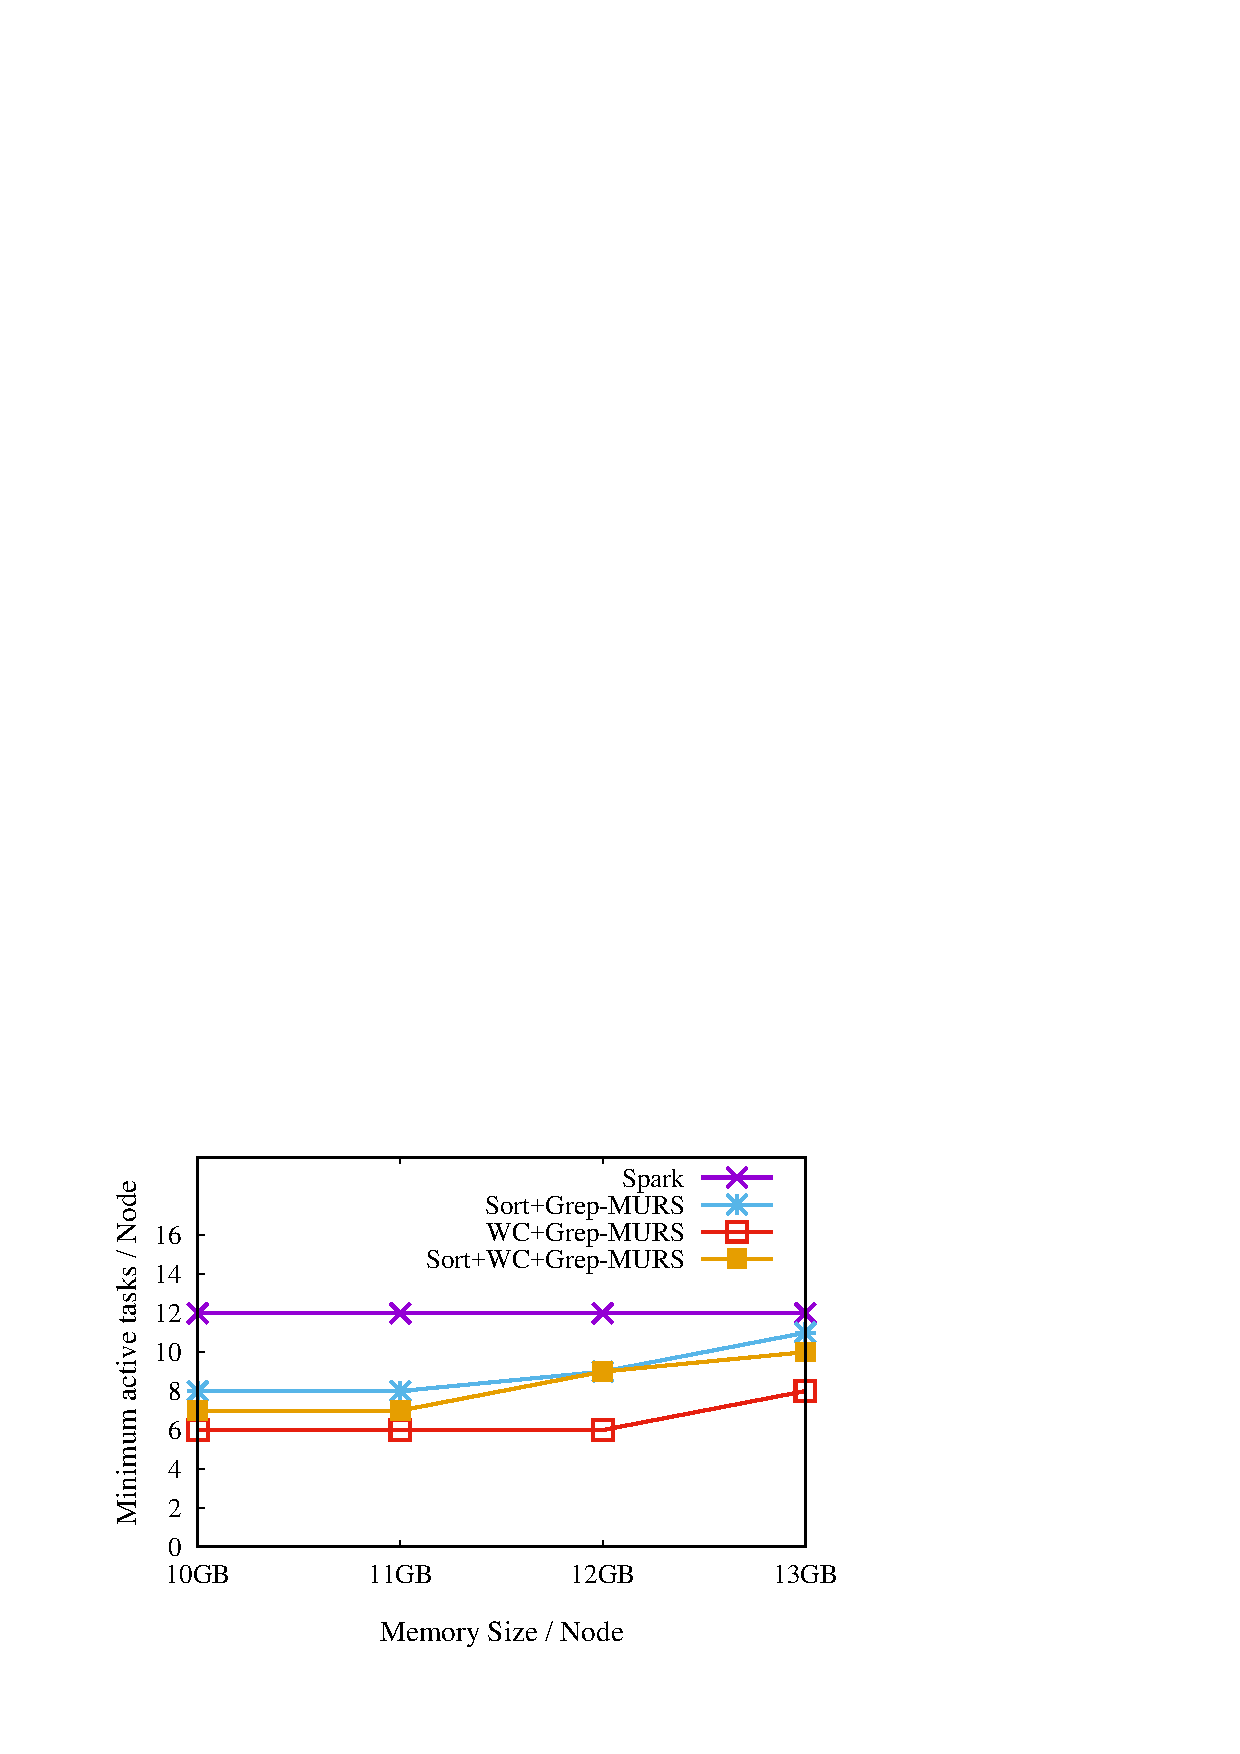
\includegraphics[width=0.3\textwidth]{active-task.pdf}}
%\vspace*{-5mm}
\caption{Results of memory pressure without caching}
%\vspace*{-4mm}
\label{fig:pressurewithoutcache}
\end{figure*}

When two applications are submitted to the server, MURS works better in Sort and Grep. Comparing Sort to WC, heavy memory pressure occurs in different phase. The \textit{sort} operation is implemented in the \textit{read phase} of tasks. Thus the tasks in the last stage of Sort suffer heavy memory pressure during their read phase. However, \textit{reduce} operation in WC is realized in the \textit{write phase} of tasks. Heavy memory pressure is resulted in by the write phase of tasks in the first stage. What's more, massive temporary data objects are produced by the function API \textit{flatMap} before the write phase. They may be currently alive in the heap during the write phase in WC. Although tasks in Sort belong to linear and tasks in WC are sub-linear based on the memory usage model, MURS suspends more tasks in WC as the heap size in WC is occupied by the temporary data objects, as shown in Figure~\ref{fig:active-task}. And these temporary data objects result in frequenter garbage collection. We can see that suspending in MURS is determined not only by the memory usage models, but also the current usage of heap. 

While three applications are submitted, out-of-memory (OME) is thrown by the server. Although the live shuffle buffer is smaller than those sever with two applications, some other data objects cost much heap space, such as the recording of living applications, the handler of disk writing, and the global configurations of Spark. Spark provides spill to avoid the shortage of memory. However, it cannot completely avoid the OME.

MURS mitigates memory pressure in each application and we find that the performance slows down tardily along with the heap size. The result shows that the cost of garbage collection is stable. As MURS suspends the heavy tasks, the tardily increasing cost in execution time is the computation time actually.  

\begin{figure}[!t]
\centering
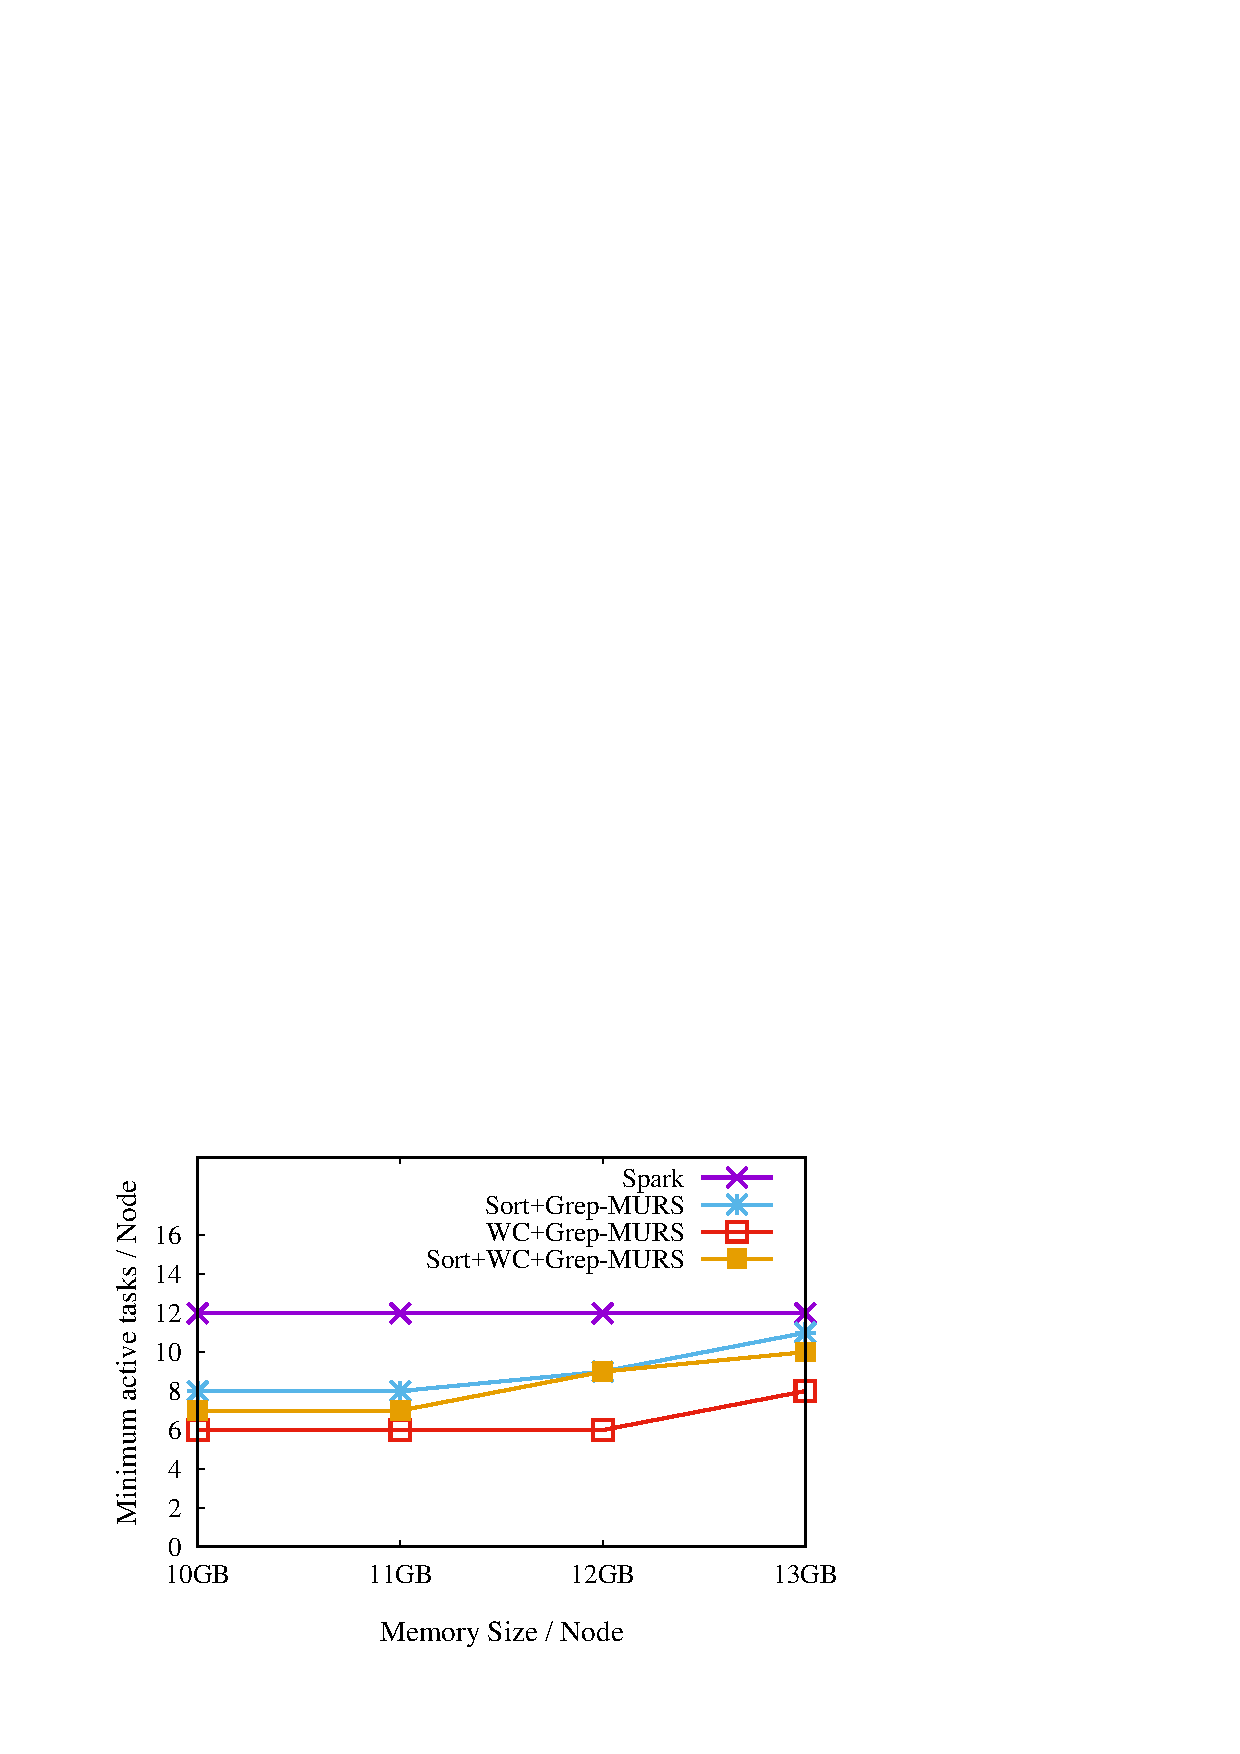
\includegraphics[width=0.35\textwidth]{active-task.pdf}
%\vspace{-2mm}
\caption{The minimum active tasks in each server}
%\vspace{-4mm}
\label{fig:active-task}
\end{figure}

\subsection{Memory pressure with caching}

Some frameworks provide caching mechanism for in-memory computation, such as Spark and Flink. Although the in-memory caching data speed up the execution of a job, some works~\cite{bu:bloat, nguyen2015facade} show that it results in greater memory pressure because the caching data live along with the job. Tracing these data is expensive and there is less accessible memory space for execution.

We choose PR and WC as the submitted applications. PR is an iterative application and we run 5 iterations in our experiments. PR caches intermediate data in memory after the first iteration. WC is submitted at the second iteration. We adjust the heap size to show the performance of MURS, while the input dataset is 30GB, as shown in Figure~\ref{fig:cache-total}. When the heap size is less than 17GB, Spark in server will throw Out-of-Memory error (OME). MURS can provide server although the heap size is reduced to 15GB. While they are both working, MURS improves the performance by up to 23.4\%, and the mitigation of memory pressure achieve a 65.4\% improvement.

\begin{figure}[!t]
\centering
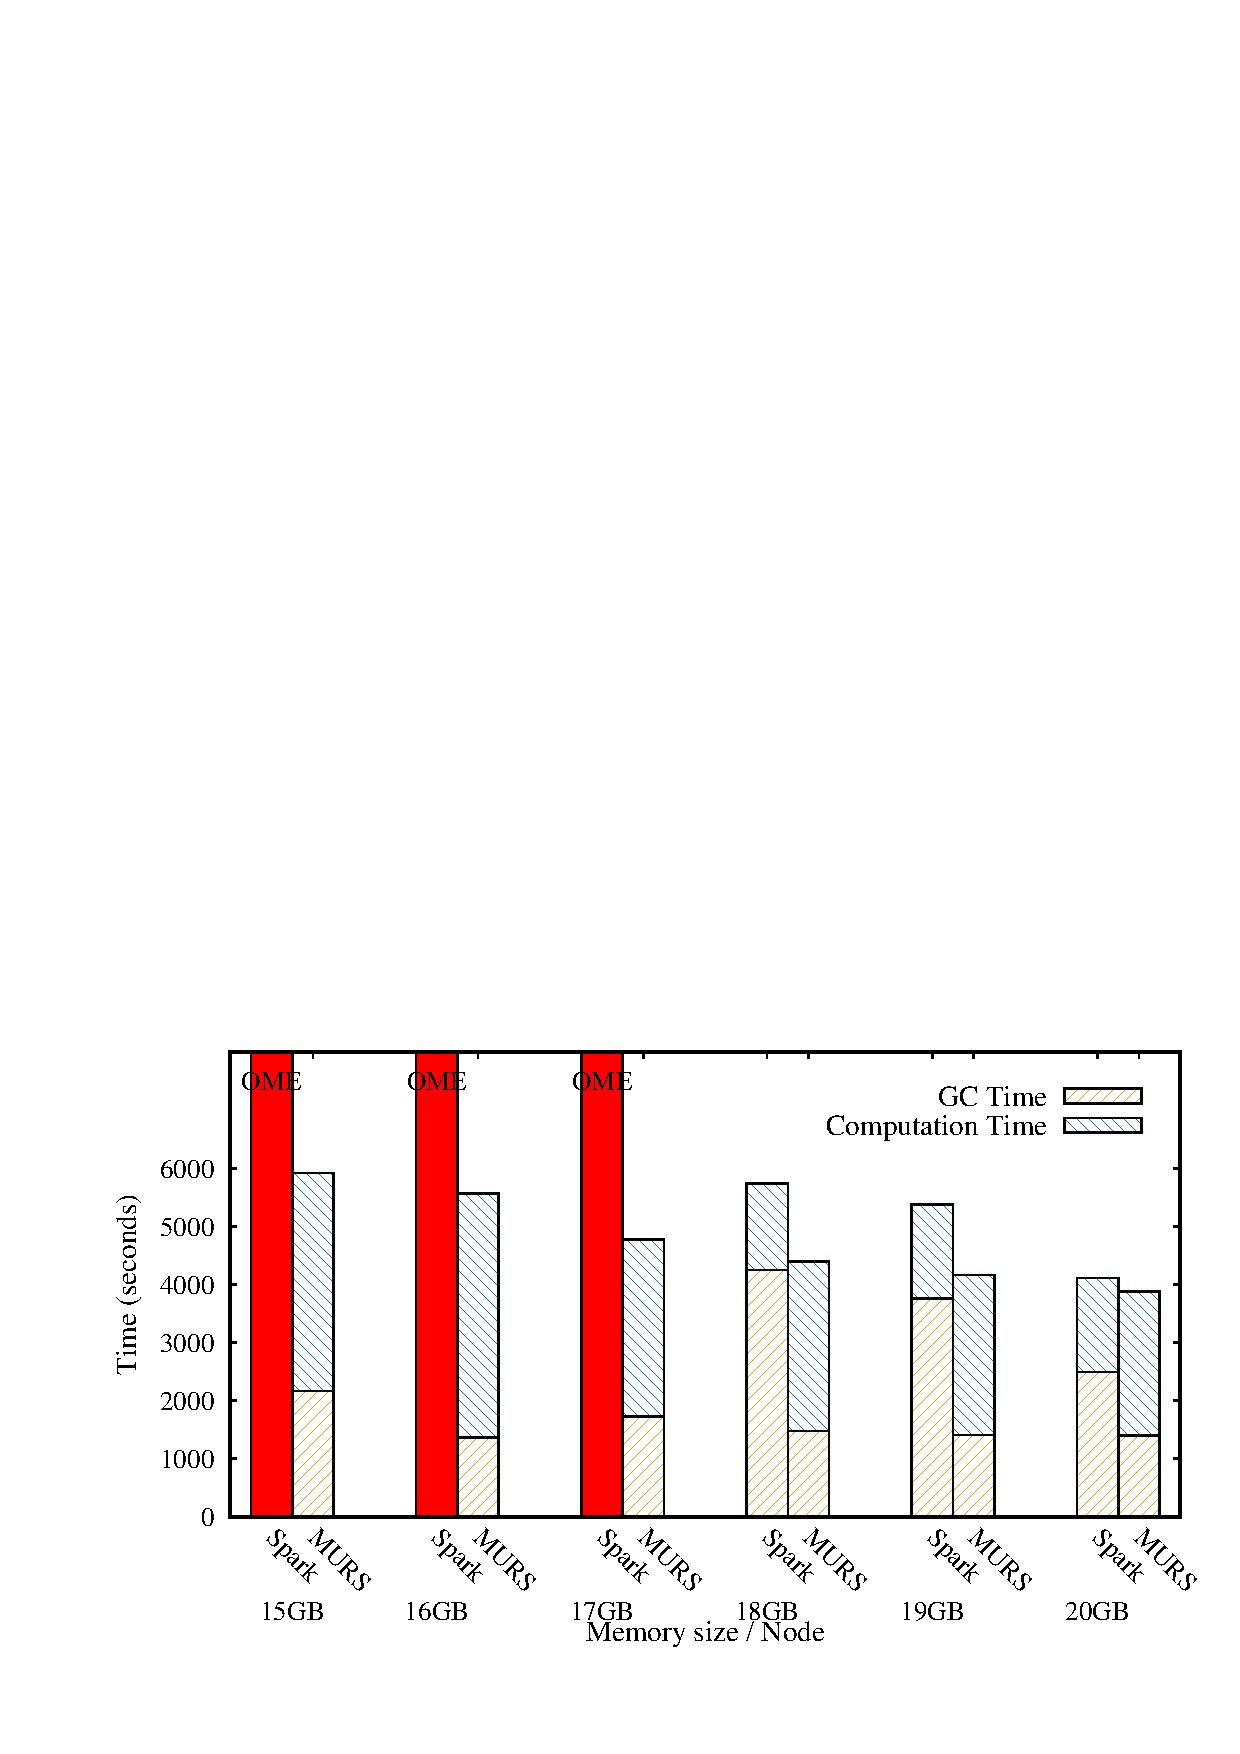
\includegraphics[width=0.45\textwidth]{cache-total.pdf}
%\vspace{-2mm}
\caption{The Execution and GC Time of PR and WC in Server}
%\vspace{-4mm}
\label{fig:cache-total}
\end{figure}

Less heap size in each node means more memory pressure in the server. When the heap is exhausted, tasks will throw the OME. With the caching data in memory, Spark for server throws the OME as the heap size of each node is 17GB. However, MURS is committed to mitigate the heavy memory pressure and still working well although the heap size of each node reduces to 15GB. MURS suspends heavy tasks to reduce the active tasks, thus running tasks can utilize more memory. Figure~\ref{fig:cache-peak} shows that the peak memory usage of all tasks in MURS persists to be larger than Spark. And the minimum tasks in MURS is reduced to ensure the available memory for running tasks. In other words, MURS has stronger scalability than Spark for server.

\begin{figure}[!t]
\centering
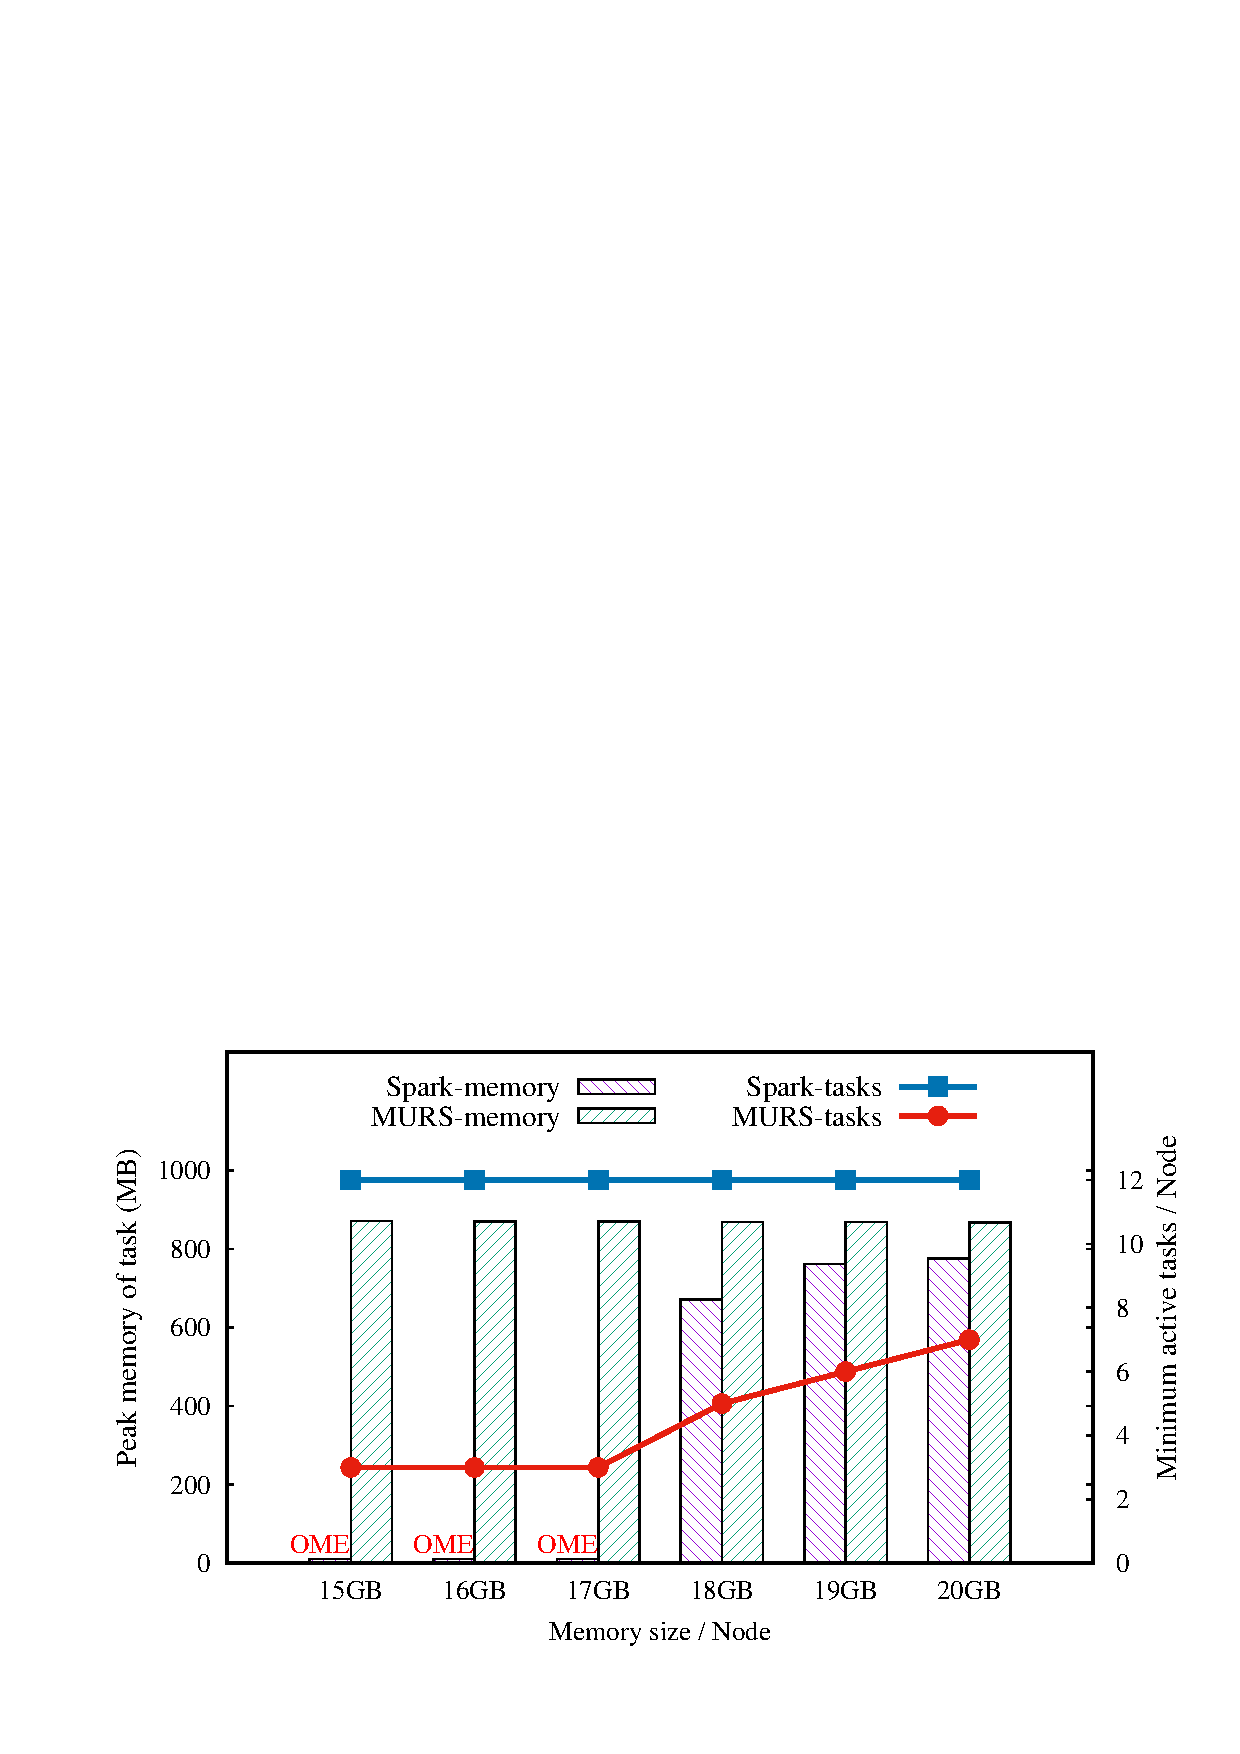
\includegraphics[width=0.45\textwidth]{cache-peak.pdf}
%\vspace{-2mm}
\caption{The peak usage memory of tasks and minimum active tasks}
%\vspace{-4mm}
\label{fig:cache-peak}
\end{figure}

\subsection{Potential starvation in MURS}

Note that the mitigation of memory pressure leads to the delay in computation. This will lead to potential starvation in suspended tasks. Fortunately, MURS solve this problem in the application level. We take the same configurations in the previous subsection. While PR and WC are submitted to the server, tasks of PR have the same \textit{write phase} as tasks of WC. But they contain more function APIs. Thus tasks of PR are mostly classified as heavy tasks. They will be suspended when the memory pressure is heavy. The execution time of each application is shown in Figure~\ref{fig:cache-prwc}. The result shows no starvation in PR, and PR is also benefit from MURS and the performance is improved by up to 24.4\%. The performance in WC which has light tasks also achieves a 29.8\% improvement. 

\begin{figure}[!t]
\centering
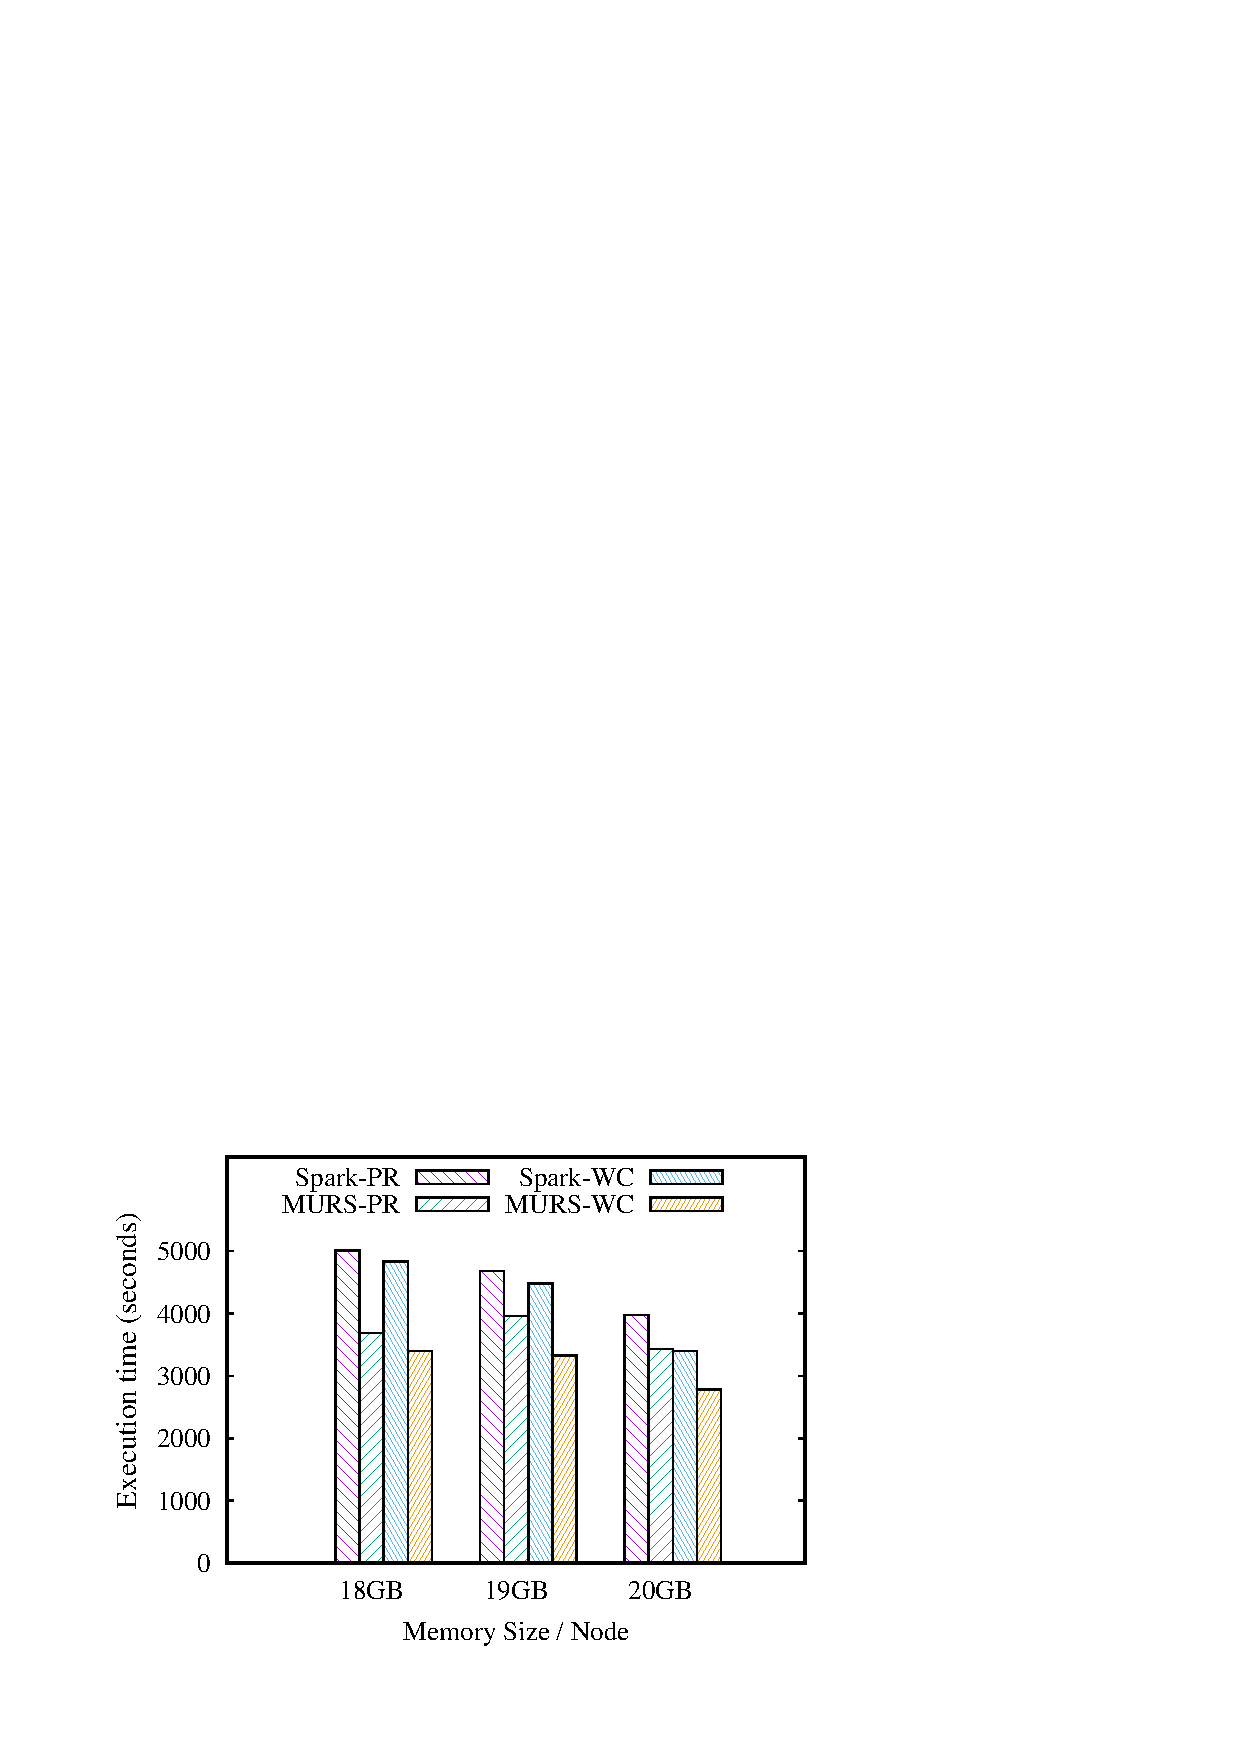
\includegraphics[width=0.35\textwidth]{cache-prwc.pdf}
%\vspace{-2mm}
\caption{The execution time of each application}
%\vspace{-4mm}
\label{fig:cache-prwc}
\end{figure}

MURS provides FIFO algorithm when it resumes the suspended tasks. This avoids the long wait of these tasks. Otherwise, suspending these tasks is to mitigate the memory pressure, not only for the current running light tasks but also the next running heavy tasks. In the application level, transient suspending and lighter memory pressure are actually trade-off. 

\subsection{Avoidance of spill}

MURS sets the red value to avoid spill when memory pressure is heavy in these systems who provide spill. We take the evaluation in the last section, which runs PR and WC in the Spark for service, to measure the spill tasks. MURS estimates the size of required memory space for each task, and ensures that running tasks can complete with the remaining memory space. As the estimation is inaccurate to some extent, we find that fewer tasks will still spill in MURS, as shown in Table~\ref{table:spill}. There are no spill tasks in WC in MURS and the spill tasks in PR decreased from 32\% to 2.5\% in comparing to Spark.

\begin{table}[!t]
\small
\centering
\caption{Spill Tasks in MURS and Spark}
\begin{tabular}{ c | c | c | c | c | c | c | c }

\hline
\multirow{2}{*}{} & \multirow{2}{*}{\textbf{App}} & \multicolumn{3}{| c |}{\textbf{Spill Percentage}} & \multicolumn{3}{| c }{\textbf{Spill Size (MB)}} \\
\cline{3-8}
 & & total & spill & percent & min & mid & max \\
\hline
\multirow{2}{*}{Spark} & WC & 1000 & 91 & 9\% & 0 & 0 & 710 \\
\cline{2-8}
 & PR & 1500 & 480 & 32\% & 310 & 367 & 439 \\
\hline
\multirow{2}{*}{MURS} & WC & 1000 & 0 & 0\% & - & - & -  \\
\cline{2-8}
 & PR & 1500 & 37 & 2.5\% & 0 & 0 & 458 \\
\hline

\hline
\end{tabular}
%\vspace{-2mm}
 
%\vspace{-6mm}
\label{table:spill}
\end{table}

We should acknowledge that error exists in the avoidance of spill. The sampler in MURS counts two important metrics of one task: the percentage of processed records in total records, and the current allocated memory space for this task. We can quickly get the required memory space based on these two metrics. When memory pressure reaches the red value, we suspend parts of tasks and leave enough remaining memory space for running tasks. As the estimate is based on sampling, error exists in the estimated size of allocated memory space, especially when the value in some key-value pairs is a collection. Different records have different sizes because the number of values inside a collection is different, such as \textit{groupByKey} in PR. Some hot keys may result in substantial error. Thus, it can be accepted that there are even fewer spill tasks in MURS.

















\begin{comment}

\subsection{Configuration}

We use four nodes as workers and one node as the master in the experiments. Each node has two eight-core Xeon-2670 CPUs and 64GB memory. The file system is mount on one SAS disk, running RedHat Enterprise Linux 5 (kernel 2.6.18). The JDK version is 1.7.0 for Spark 1.6 and Spark Job Server 0.6.2. We count not only the execution time of each application, but also the details of all tasks. Some important configurations are set to be the same in both MURS and Spark, as shown in Table~\ref{table:config}. The memory of each executor is set to be 15GB.

\begin{table}[!t]
\small
\centering
\caption{Important Configurations in MURS and Spark}
\begin{tabular}{ c | c | c }

\hline
\textbf{Configurations} & \textbf{Default} & \textbf{Value} \\
\hline
spark.serializer & No & KryoSerializer \\
\hline
spark.cores.max & No & 48 \\
\hline
spark.shuffle.compress & Yes & true \\
\hline
spark.shuffle.manager & Yes & sort \\
\hline
spark.memory.fraction & Yes & 0.75 \\
\hline
spark.memory.storageFraction & Yes & 0.5 \\
\hline

\hline
\end{tabular}
%\vspace{-2mm} 
%\vspace{-6mm}
\label{table:config}
\end{table} 

We choose four typical benchmark applications in Spark to evaluate the performance: Grep, Sort, WordCount(WC), and PangeRank(PR). Grep has only one stage: it filters the records that do not satisfy the conditions. WC has two stages: it counts the number of each key in the input file.  Sort has three stages: it sorts all records by key in the input file. While PR is a typical iterative computations, and one of its most important features is that it will cache data in memory. We choose these four benchmarks because these applications contains all three models. We will show the details later. For Grep, Sort, and WC, the datasets are produced by HiBench Random Writer with different unique key numbers (1M and 1B), both with the size of 50GB. And for PR, we use the real graphs: webbase-2001 (30GB)~\cite{boldi:webgraph} to evaluate the performance of MURS. Key-value pairs of each record in all input dataset have the similar size, thus we can simply analyze the memory usage model by function API. These applications are grouped to evaluate different scenes and submitted to Spark Job Server together.

\subsection{Memory pressure without caching}

Most current data processing systems are designed based on MapReduce, but only parts of them provide the in-memory computing model that caches data in memory to speed up the system. Thus, we first evaluate these applications without caching data in memory to stand for common frameworks working with key-value pairs, such as Hadoop and Hive.

We choose Grep, Sort, and WC to form the benchmark set. The function APIs in each job are shown in Table~\ref{table:grep-sort-wc}. Grep has no shuffle operation. WC and Sort jobs are split by the shuffle operations. Tasks in the first stage of WC result in more memory pressure than second stage, because most records are aggregated in the write phase. In contrast, Sort actually sorts keys in the read phase of tasks in the third stage. Jobs are simultaneously submitted to Spark Job Server. The execution time of each job is decreased by 20\% to 30\%. We count the execution time and garbage collection time of all tasks in each stage, as shown in Figure~\ref{fig:grep-sort-wc-gc}. Tasks with constant model (Stage 2-3) all have a short execution time. They also benefit from MURS and the execution time is decreased by 59\%, although the garbage collection time of them has less degradation. Execution time of tasks with sub-linear model (Stage 0) is decreased by 54\% and the reduction comes all from the mitigation of garbage collection. Execution time of tasks with linear model (Stage 5) is reduced by 50\%, and the garbage collection time is decreased by 58\%.

\begin{table}[!t]
\small
\centering
\caption{Function APIs in each Application without caching}
\begin{tabular}{ c | c | c | c }

\hline
\textbf{Application} & \textbf{Stage ID} & \textbf{Function API} & \textbf{Model}\\
\hline
\multirow{2}{*}{WC} & Stage 0 & \textit{reduceByKey} & sub-linear  \\
\cline{2-4}
 & Stage 1 & \textit{reduceByKey} & sub-linear \\
\hline
Grep & Stage 2 & \textit{filter} & constant \\
\hline
\multirow{3}{*}{Sort} & Stage 3 & \textit{flatMap} & constant \\
\cline{2-4}
 & Stage 4 & \textit{sortByKey} & linear \\
\cline{2-4}
 & Stage 5 & \textit{sortByKey} & linear \\
\hline

\hline
\end{tabular}
%\vspace{1mm} 
%\vspace{-8mm}
\label{table:grep-sort-wc}
\end{table}

%We chose Grep, Sort, and WC to group the submitted jobs. The function API in Grep is \textit{filter}, which does not distinguish the key and process each record. It just judges whether the record satisfies given conditions and writes it to disk; thus, all data objects are temporary data objects and the model belongs to the constant model. The function API in Sort is \textit{sortByKey}, which must shuffle all records and partition the records in order by key. Each record will be saved in shuffle buffer before writing to disk, thus it belongs to the linear model. The function API in WC is \textit{reduceBykey}, which distinguishes the key and aggregates the value. It is a typical sub-linear model. From the model, we find that tasks in Sort may have more impact on memory pressure. The result shows that the execution time of WC is decreased by 20\%, Grep is decreased by 15\%, and Sort is decreased by 13\%. We take the execution time and garbage collection time of tasks to analyze the improvement, as shown in Figure~\ref{fig:grep-sort-wc-gc}.

\begin{figure}[!t]
\centering
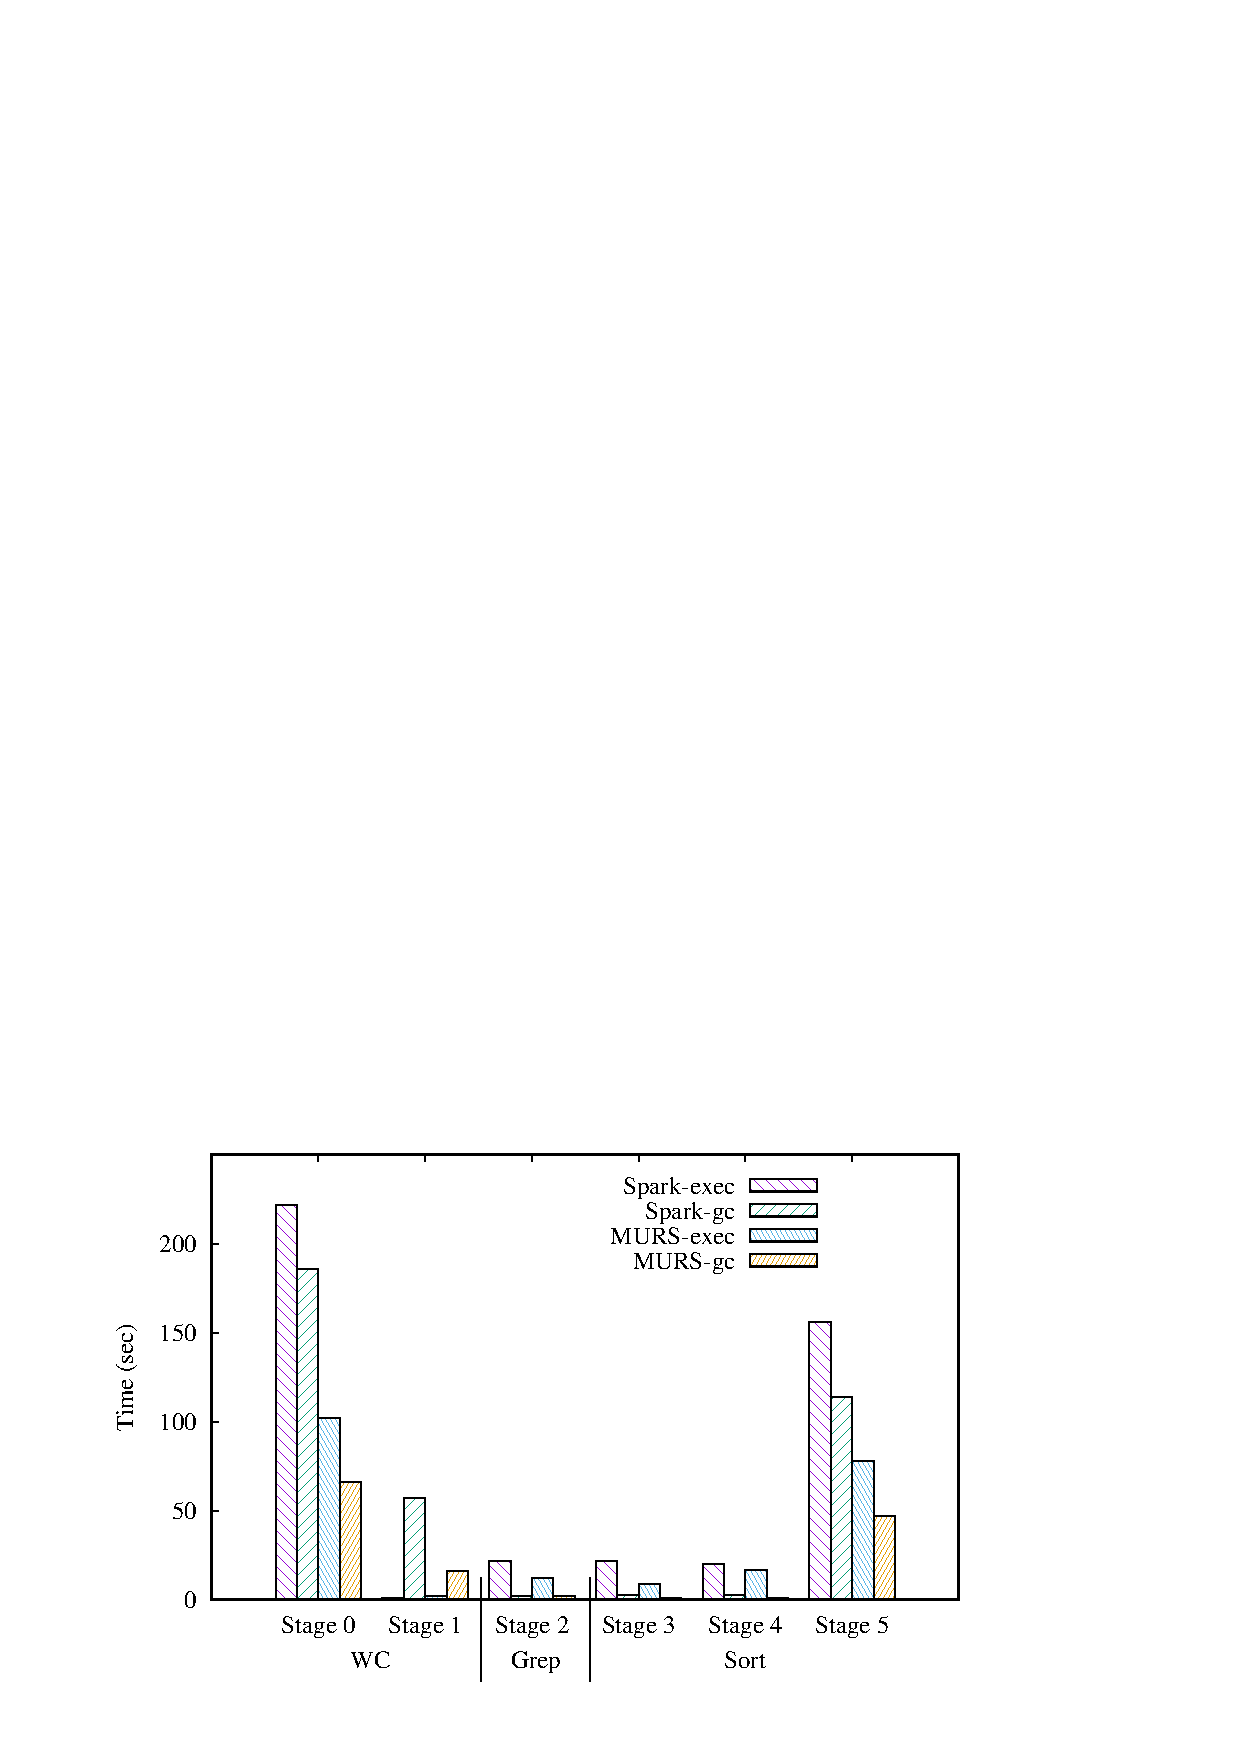
\includegraphics[width=0.4\textwidth]{grep-sort-wc-gc.pdf}
%\vspace{-2mm}
\caption{The Execution and GC Time of Tasks in Sort, Grep and WC}
%\vspace{-4mm}
\label{fig:grep-sort-wc-gc}
\end{figure}

Tasks with constant model in Stage 2 and Stage 3, along with tasks with sub-linear model in Stage 1, all benefit from MURS although the memory pressure is light. This is due to the parallelism in writing to disk, as Spark writes intermediate data in shuffle write phase to disk for checkpoint. Note that when these tasks are running, tasks in Stage 5 have not been launched. MURS is triggered when the proportion of used heap first touch the yellow value, it suspends some tasks in WC and decreases the parallelism in writing to disk. With enough bandwidth of writing to disk, these tasks still execute fast. We find that tasks in Stage 4 benefit less from the parallelism in writing to disk, because they are linear models and suspended by MURS when the proportion of used heap touches the yellow value. 

The reductions of Stage 0 and Stage 5 prove the mitigation on memory pressure through MURS. The garbage collection time in WC has a greater degradation than Sort. While WC suffers heavy memory pressure produced by Sort in Spark, MURS suspends tasks with linear models in Sort and ensures enough memory space for WC. Almost all reduction time comes from the mitigated memory pressure because there are no suspended tasks in WC. Sort gets more memory space after WC completes, and has less memory pressure than Spark. 

%As the Sort application is split into three stages, only tasks in the second stage (this stage just prepares records for the next stage and writes records to disk) and the third stage (this is the actual stage that sorts the key) is the linear model. The function API in the first stage is \textit{flatMap}, which flats the result and provides an iterator, thus it belongs to the constant model. We find that these tasks with sub-linear and linear models suffer greater memory pressure, and all benefit from MURS. However, we can see that the constant model is also a little better, although the garbage collection time has a lower percentage in the original execution time—such as tasks in Grep and the first stage of Sort. This is due to the parallelism in writing to disk. As other tasks suffer heavy memory pressure, MURS stops some tasks and prevents them from writing shuffle data to disk. The accessibility of the disk can be faster, and those running tasks with the constant model can quickly complete their operation on disk. 

\subsection{Memory pressure with caching}

Some frameworks provide caching mechanism for in-memory computation, such as Spark and Flink. Although the in-memory caching data speed up the execution of a job, some works~\cite{bu:bloat, nguyen2015facade} show that it results in greater memory pressure because the caching data live along with the job. Tracing these data is expensive and there is less accessible memory space for execution.

PR is an example of iterative computations that caches important intermediate data in memory. The function API in the first stage of PR is \textit{groupByKey}, which groups all values of the particular key without aggregation. The result of \textit{groupByKey} will be cached in memory and used in subsequent iterations. Thus, the memory usage models of these tasks are linear. Thus, the memory usage models of tasks in Stage 2-3 are linear.  The caching data is alive in memory until the job is completed. Each iteration is implemented in a stage that contains several function APIs: \textit{join}, \textit{map}, and \textit{reduceByKey}. The function APIs \textit{map} and \textit{reduceByKey} are the same as that in Grep and WC. Although \textit{join} distinguishes the key, the function API here just processes the keys in one partition, which means it does not shuffle all keys. Thus, all data objects produced by \textit{join} are temporary data objects, and the sampler will classify it as the constant model. We submit PR along with WC, similarly to Section~\ref{sec:motivation}. The result is shown in Figure~\ref{fig:pr-wc-exec}. We should notice that, when WC job completes, PR is running in Stage 3. During the process of WC, the execution time of WC job is decreased by 28\%, but at the same time the execution time of PR job increased by 26\%. After WC is complete, the execution time of PR job can be decreased by 58\%.

\begin{figure}[!t]
\centering
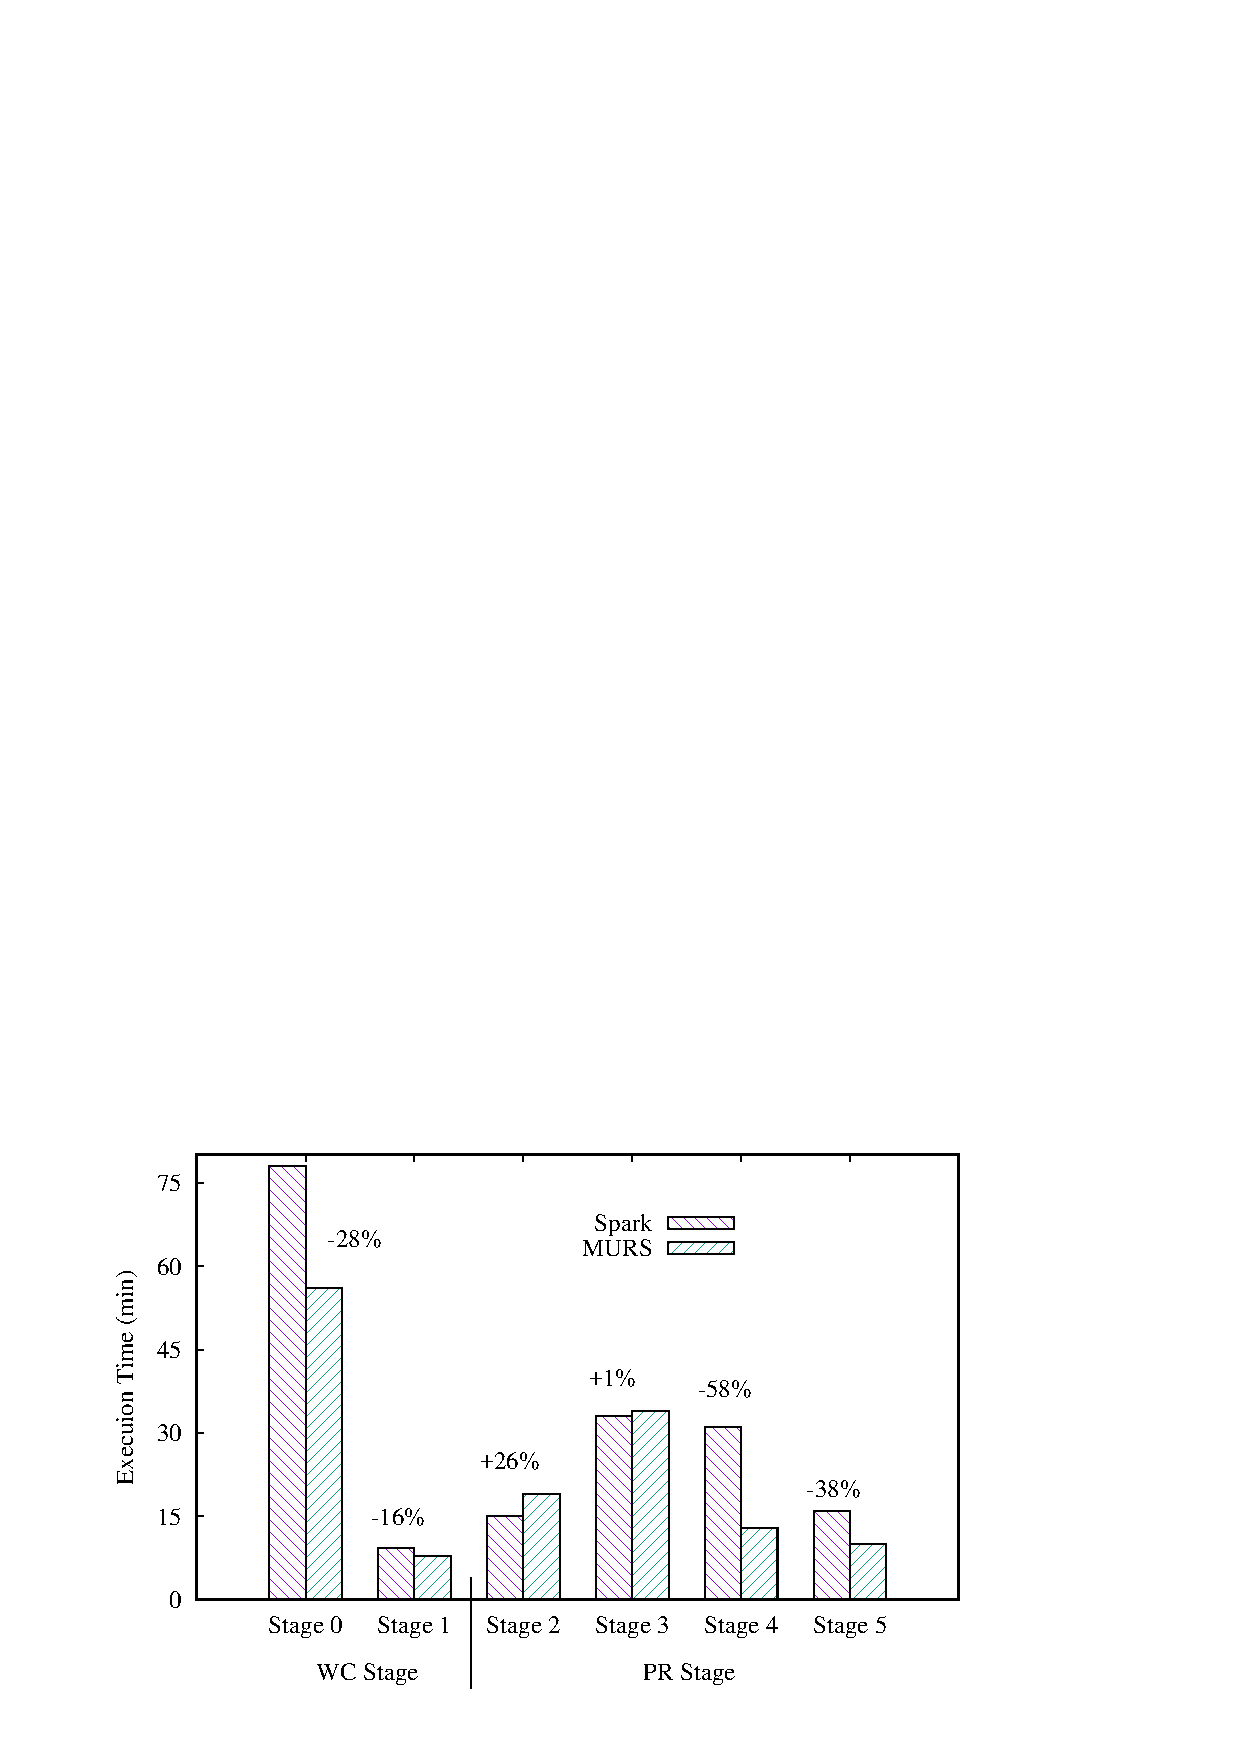
\includegraphics[width=0.4\textwidth]{multitalent-exec.pdf}
%\vspace{-2mm}
\caption{The Execution Time of PR Job and WC Job}
%\vspace{-4mm}
\label{fig:pr-wc-exec}
\end{figure}

\begin{figure}[!t]
\centering
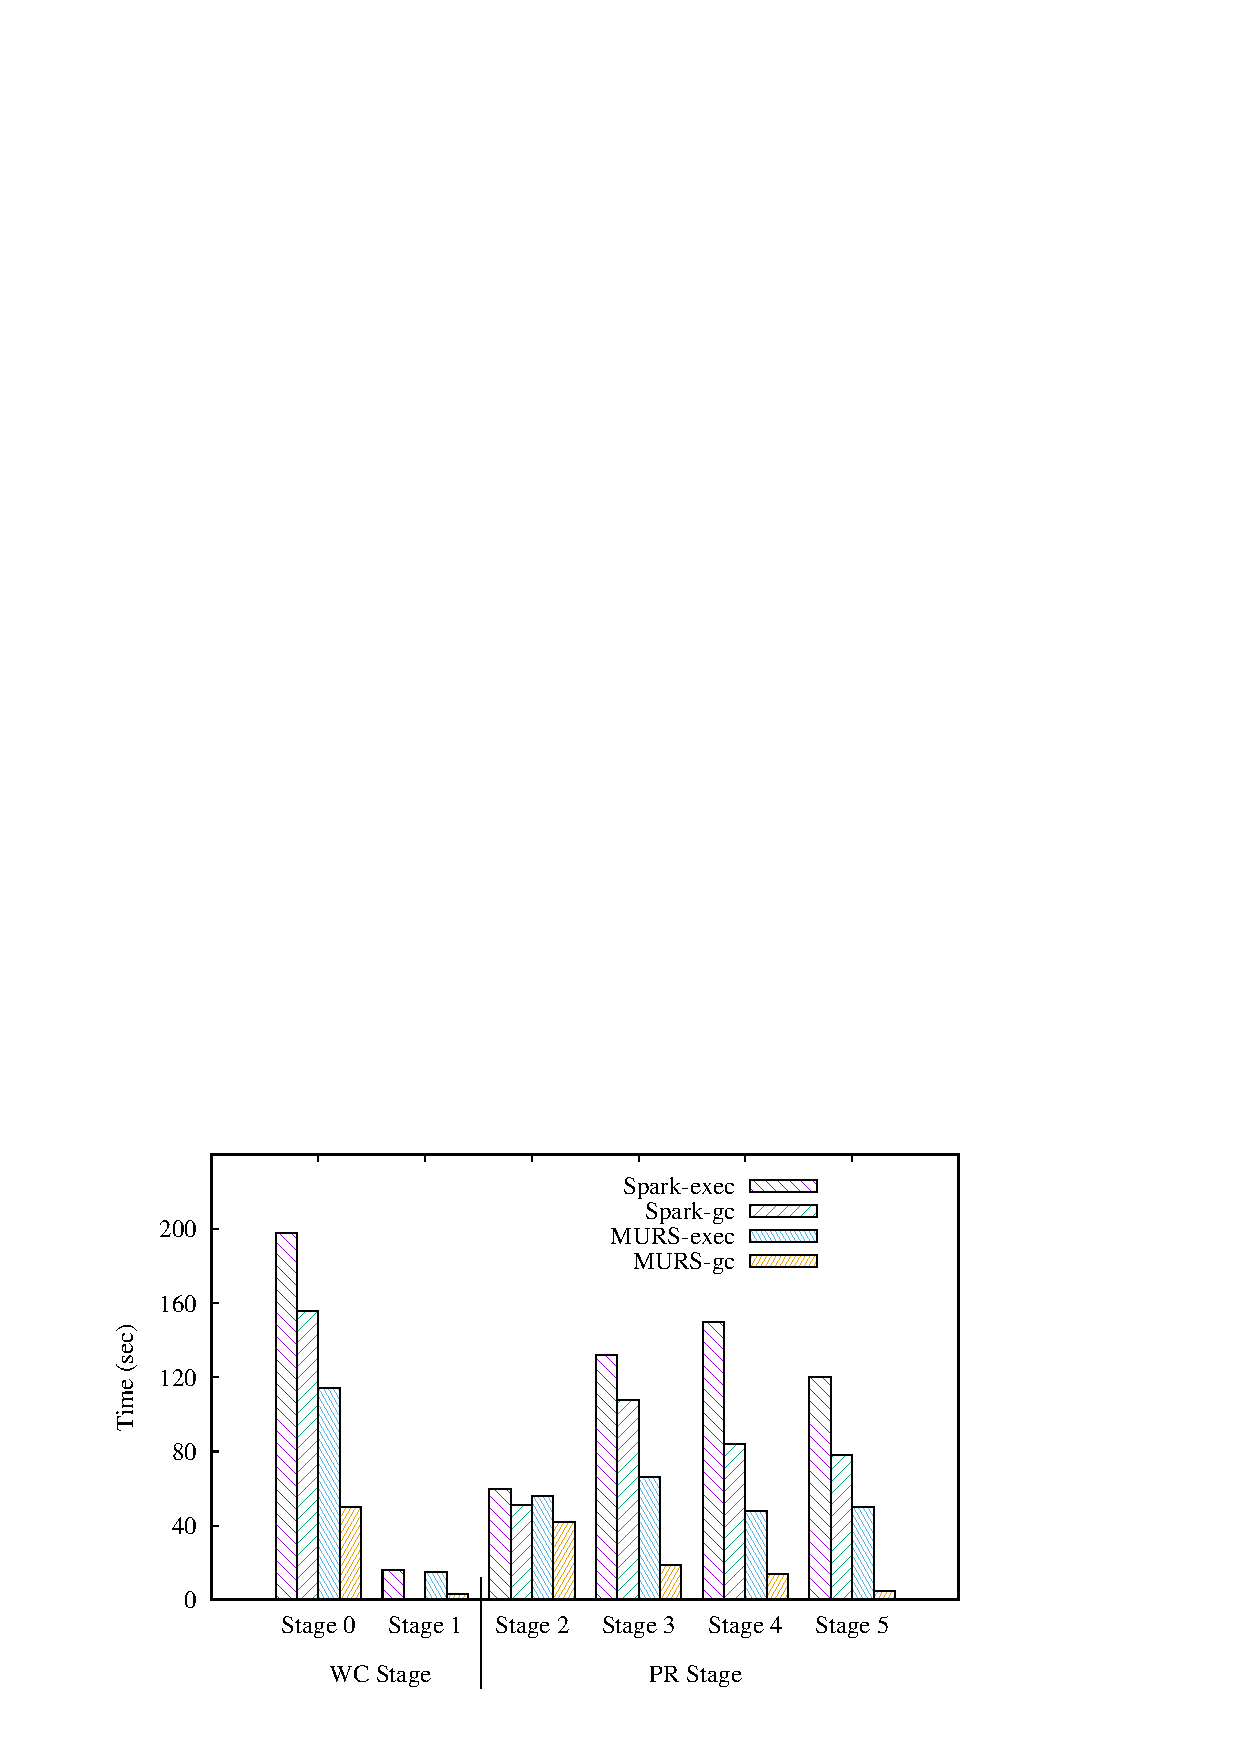
\includegraphics[width=0.4\textwidth]{pr-wc-gc.pdf}
%\vspace{-2mm}
\caption{The Execution and GC Time of Tasks in PR and WC}
%\vspace{-4mm}
\label{fig:pr-wc-gc}
\end{figure}

Before WC completes, tasks in PR and WC both result in memory pressure. However, tasks in PR belong to linear model, while tasks in WC belong to sub-linear model. MURS will suspend these tasks in PR to prevent heavy memory pressure, thus tasks in WC can have a lower execution time.

The execution time of the second stage of PR increases because tasks in PR are always classified to heavy tasks in this scene. In the second stage, PR caches all intermediate data in memory until the job completes. Then the memory manager requires many CPU cycles to trace the caching data objects; and less memory space is accessible for execution, which results in heavy garbage collection. While MURS intends to mitigate the heavy memory pressure, tasks in PR are always classified to heavy tasks because there are no other tasks belong to linear models. Thus, the waiting time of suspended tasks increases greatly although the garbage collection time decreases in Figure~\ref{fig:pr-wc-gc}, and the second stage in PR is even worse in MURS than in Spark for service. Fortunately, as WC completes early, subsequent stages  in MURS suffer much less memory pressure (the garbage collection can be decreased as much as 94\% in some tasks in Figure~\ref{fig:pr-wc-gc}), and performance improves more. 

\subsection{Avoidance of spill}

MURS sets the red value to avoid spill when memory pressure is heavy in these systems who provide spill. We take the evaluation in the last section, which runs PR and WC in the Spark for service, to measure the spill tasks. MURS estimates the size of required memory space for each task, and ensures that running tasks can complete with the remaining memory space. As the estimation is inaccurate to some extent, we find that fewer tasks will still spill in MURS, as shown in Table~\ref{table:spill}. There are no spill tasks in WC in MURS and the spill tasks in PR decreased from 32\% to 2.5\% in comparing to Spark.

\begin{table}[!t]
\small
\centering
\caption{Spill Tasks in MURS and Spark}
\begin{tabular}{| c | c | c | c | c | c | c | c |}

\hline
\multirow{2}{*}{} & \multirow{2}{*}{\textbf{App}} & \multicolumn{3}{| c |}{\textbf{Spill Percentage}} & \multicolumn{3}{| c |}{\textbf{Spill Size (MB)}} \\
\cline{3-8}
 & & total & spill & percent & min & mid & max \\
\hline
\multirow{2}{*}{Spark} & WC & 1000 & 91 & 9\% & 0 & 0 & 710 \\
\cline{2-8}
 & PR & 1500 & 480 & 32\% & 310 & 367 & 439 \\
\hline
\multirow{2}{*}{MURS} & WC & 1000 & 0 & 0\% & - & - & -  \\
\cline{2-8}
 & PR & 1500 & 37 & 2.5\% & 0 & 0 & 458 \\
\hline

\hline
\end{tabular}
%\vspace{-2mm}
 
%\vspace{-6mm}
\label{table:spill}
\end{table}

We should acknowledge that error exists in the avoidance of spill. The sampler in MURS counts two important metrics of one task: the percentage of processed records in total records, and the current allocated memory space for this task. We can quickly get the required memory space based on these two metrics. When memory pressure reaches the red value, we suspend parts of tasks and leave enough remaining memory space for running tasks. As the estimate is based on sampling, error exists in the estimated size of allocated memory space, especially when the value in some key-value pairs is a collection. Different records have different sizes because the number of values inside a collection is different, such as \textit{groupByKey} in PR. Some hot keys may result in substantial error. Thus, it can be accepted that there are even fewer spill tasks in MURS.

\subsection{Memory pressure in multi-launch}

Some systems for service are oversold and launches multiple tasks than the original configuration. When the service is idle, it has efficient memory usage. However, if the service comes to busy, the memory pressure is uncontrollable and the performance will degrade quickly when memory pressure is heavy. MURS is appropriate for this problem as it keeps the advantage in light memory pressure but prevents memory pressure increasing fast in heavy memory pressure. We choose WC here and two datasets to compare the impact of multi-launch MURS with Spark. We submit WC independently here to clearly distinguish the light and heavy memory pressure, and MURS can also work as mentioned in Section~\ref{sec:desgin}. WC processes data as (\textit{K}, \textit{V}), while \textit{K} means the words in the dataset. Thus, the number of words will decide the size of shuffle buffer, and more words will result in more memory pressure. As shown in Figure~\ref{fig:subfig:wc-million}, the GC time can be increased to 31.8\%, but the reduction of execution time is 11.6\% when the number of words is 1 million; the reduction of execution time is 22.9\% and the GC time can be 45.2\% when the number of words increases to 100 million in Figure~\ref{fig:subfig:wc-billion}.

%Although MURS is designed for data processing systems for service, we find it can also work well in batch processing when all running tasks have the same model. We choose WC here and two datasets to compare the impact of multi-launch in different memory pressures. WC process data as (\textit{K}, \textit{V}), while \textit{K} means the words in the dataset. Thus, the number of words will decide the size of shuffle buffer, and more words will result in more memory pressure. As shown in Figure~\ref{fig:subfig:wc-million}, the GC time can be increased to 31.8\%, but the reduction of execution time is 11.6\% when the number of words is 1 million; the reduction of execution time is 22.9\% and the GC time can be 45.2\% when the number of words increases to 1 billion in Figure~\ref{fig:subfig:wc-billion}.

\begin{figure}[!t]
\centering
\subfigure[Light memmory pressure]{
\label{fig:subfig:wc-million}
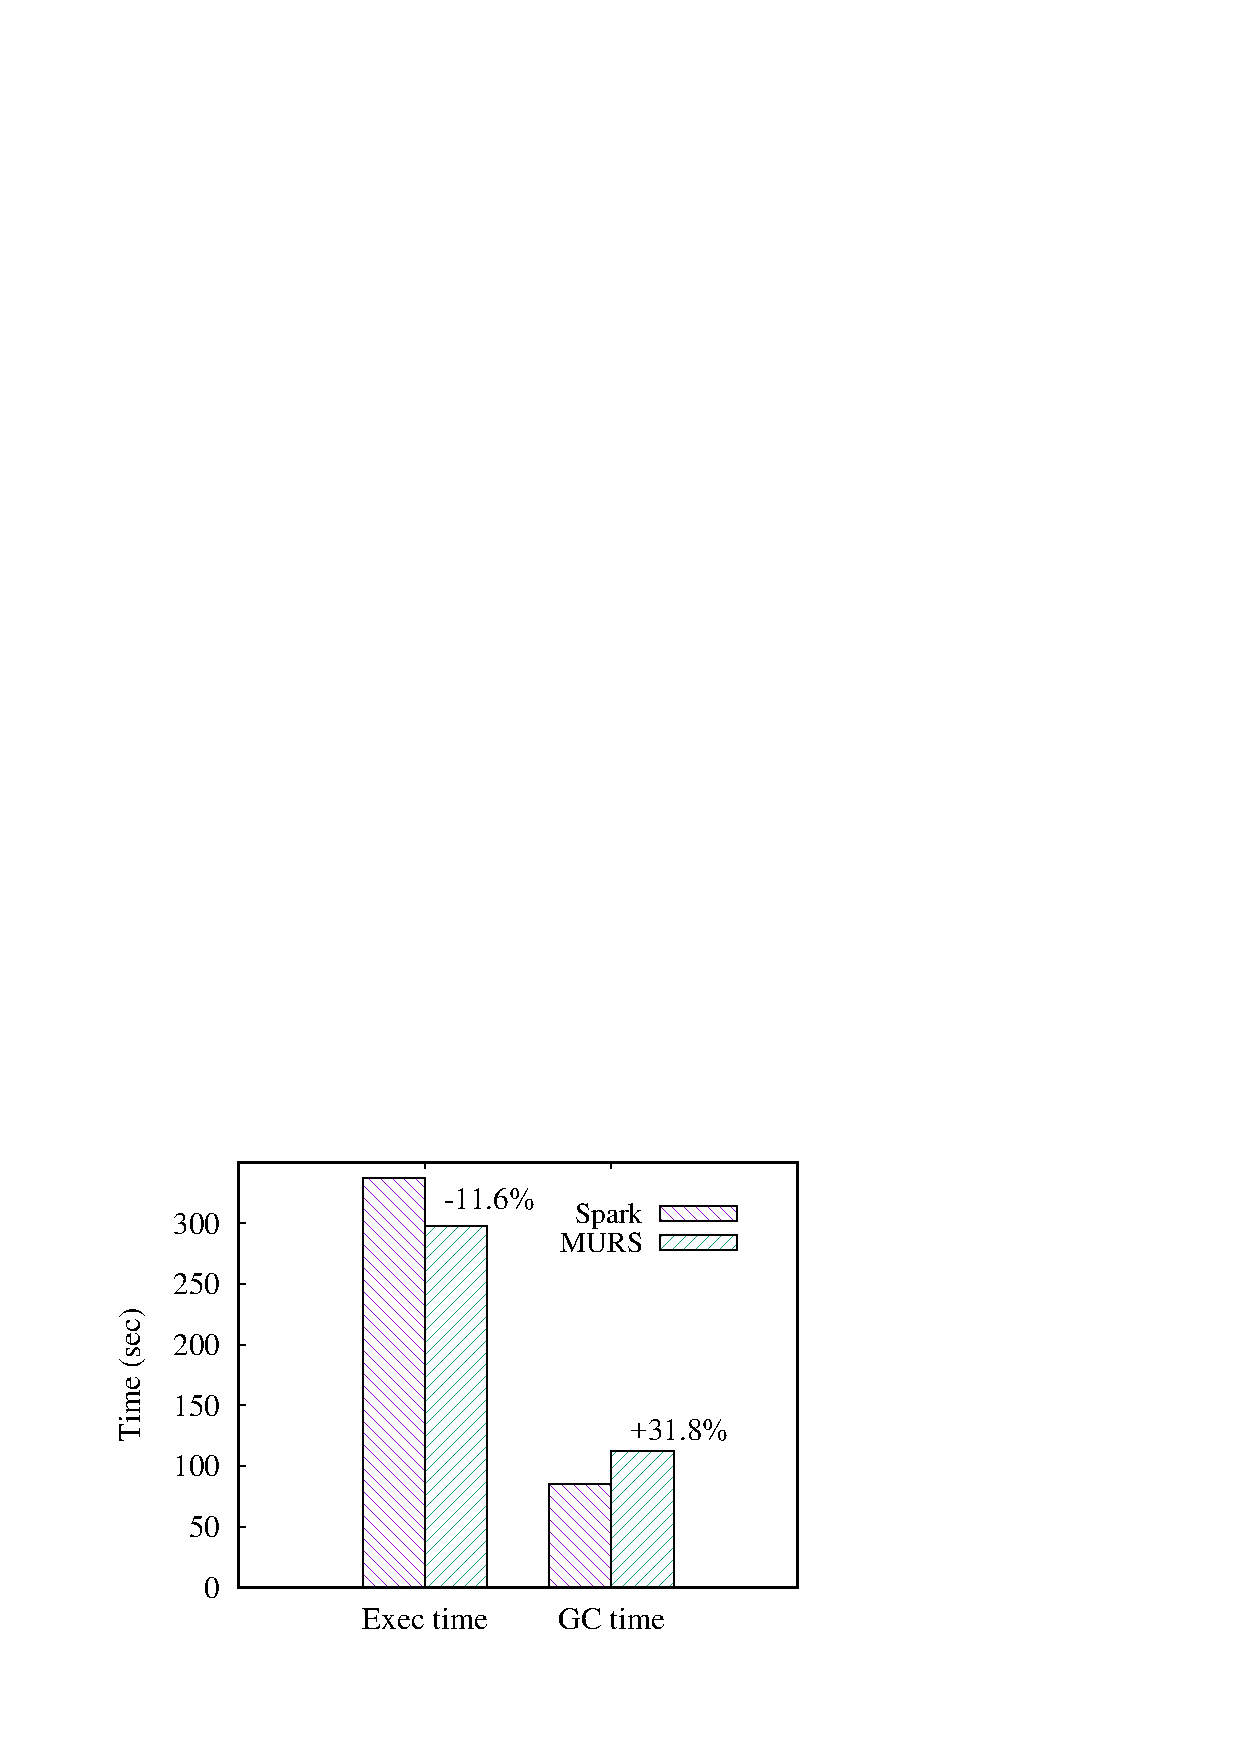
\includegraphics[width=0.231\textwidth]{wc-million.pdf}}
\hspace{-1.3ex}
\subfigure[Heavy memory pressure]{
\label{fig:subfig:wc-billion}
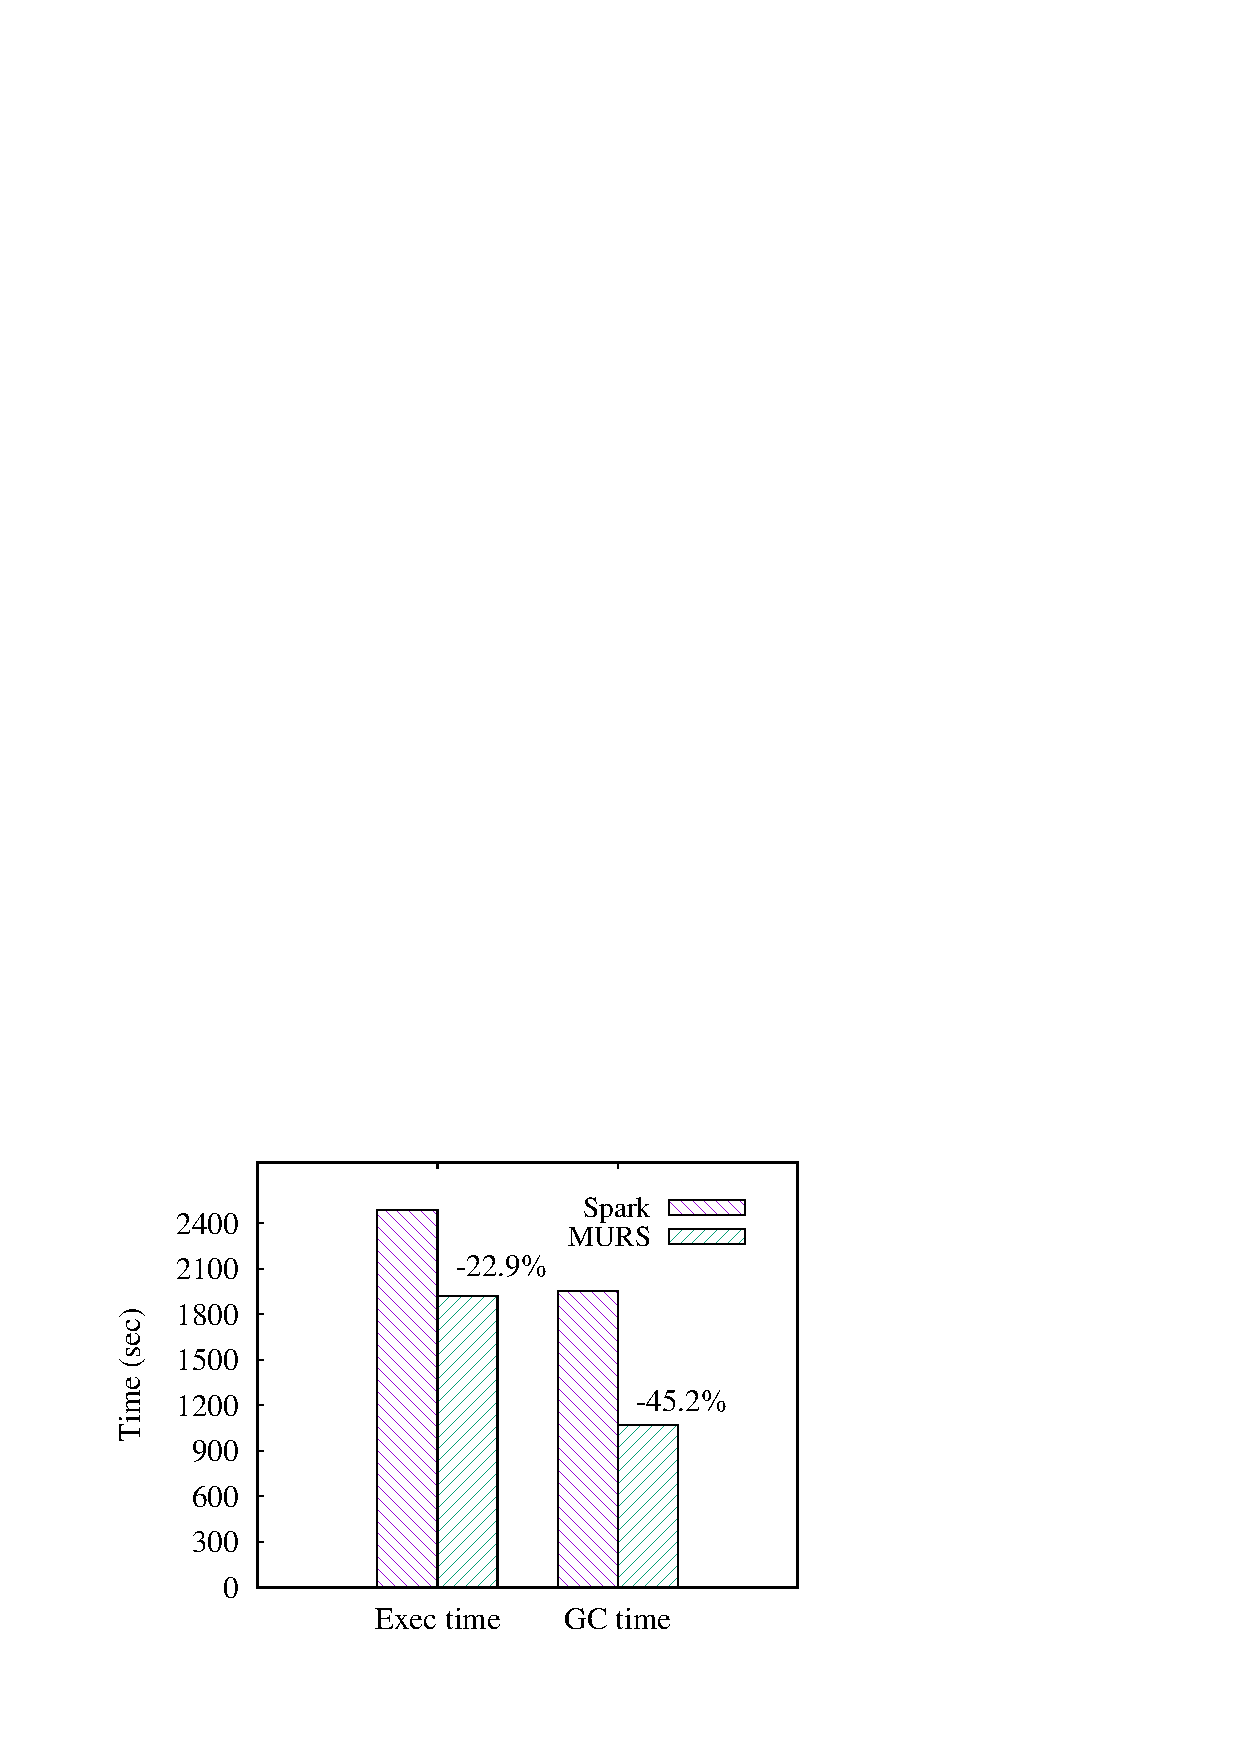
\includegraphics[width=0.231\textwidth]{wc-billion.pdf}}
\label{fig:wc-result}
%\vspace{-2mm}
\caption{Multi-launch with MURS when service is busy}
%\vspace{-4mm}
\end{figure}

Light memory pressure usually means that memory space will suffer less allocation and reclamation. Multi-launch increases the parallelism as well as the memory pressure, which properly increase the frequency of memory allocation and reclamation. This improves the efficiency of memory usage. Thus the services work well with multi-launch in Figure~\ref{fig:subfig:wc-million}. MURS remains the advantages in this scene. However, when the words increases to 100 million, memory pressure is high and the throughout is only 25.6\%. Frequent garbage collection degrades the performance quickly. MURS will suspend numbers of tasks to prevent the increase of memory pressure, thus both execution time and garbage collection time decrease in Figure~\ref{fig:subfig:wc-billion}.



















%%%%\begin{comment}

\subsection{Batch Processing}

\subsubsection{Impcat of Shuffle Function}
WordCount in Spark benchmark is an original MapReduce application. WC has two stages: the first stage reads data from HDFS and writes shuffle buffers; the second stage reads data from shuffle buffers and then function \textit{reduceByKey} is used to get the result. Shuffle buffers process data as (\textit{Key},\textit{Value}) while \textit{Key} means the words in dataset. Thus the number of words will decide the size of shuffle buffers, and more words will result in more memory pressure. As shown in Figure~\ref{fig:subfig:wc-million}, the GC time can be increased to 31.8\% but the reduction of execution time is 11.6\% when the number of words is 1 million; the reduction of execution time is 22.9\% and the GC time can be 45.2\% when the number of words increases to 1 billion in Figure~\ref{fig:subfig:wc-billion}.

When the size of words is small, the shuffle buffers will have less keys. The size of shuffle buffers will not result in heavy memory pressure which can also be proved by the light garbage collection. MURS provides multi launch to increase the memory pressure and parallelism of job, the running tasks is 1.5x than Spark. Thus the execution time decreases but the garbage collection time increases in Figure~\ref{fig:subfig:wc-million}. However, when the words increases to 1 billion, memory pressure can be high and the throughout is only 25.6\%. MURS will stop numbers of tasks to prevent the increase of memory pressure and both execution time and garbage collection time will decrease in Figure~\ref{fig:subfig:wc-billion}. 

\subsubsection{Impcat of Caching and Shuffle Function}
PageRank(PR) will firstly cache important intermediate data of function \textit{groupByKey} in memory. Each of the appending several iterations is a stage in the job. The main functions in each stage are \textit{join} and \textit{reduceByKey}. The function \textit{join} not belongs to shuffle function in PR. We test 10 iterations here and the result is shown in Figure~\ref{fig:pr-stagetime}. While the first stage just read data from HDFS, the memory pressure is light. After stages will suffer from caching data in memory. The size of caching data in each node is 4.1GB-5.3GB. Different stage has different memory pressure, the max execution time has the speed up of 2.1x to the min in Spark. Different memory pressure and tasks result in different performance of MURS. The best reduction of execution time can be 56\% and the average reduction is 44\% for computing stages.

\begin{figure}[!t]
\centering
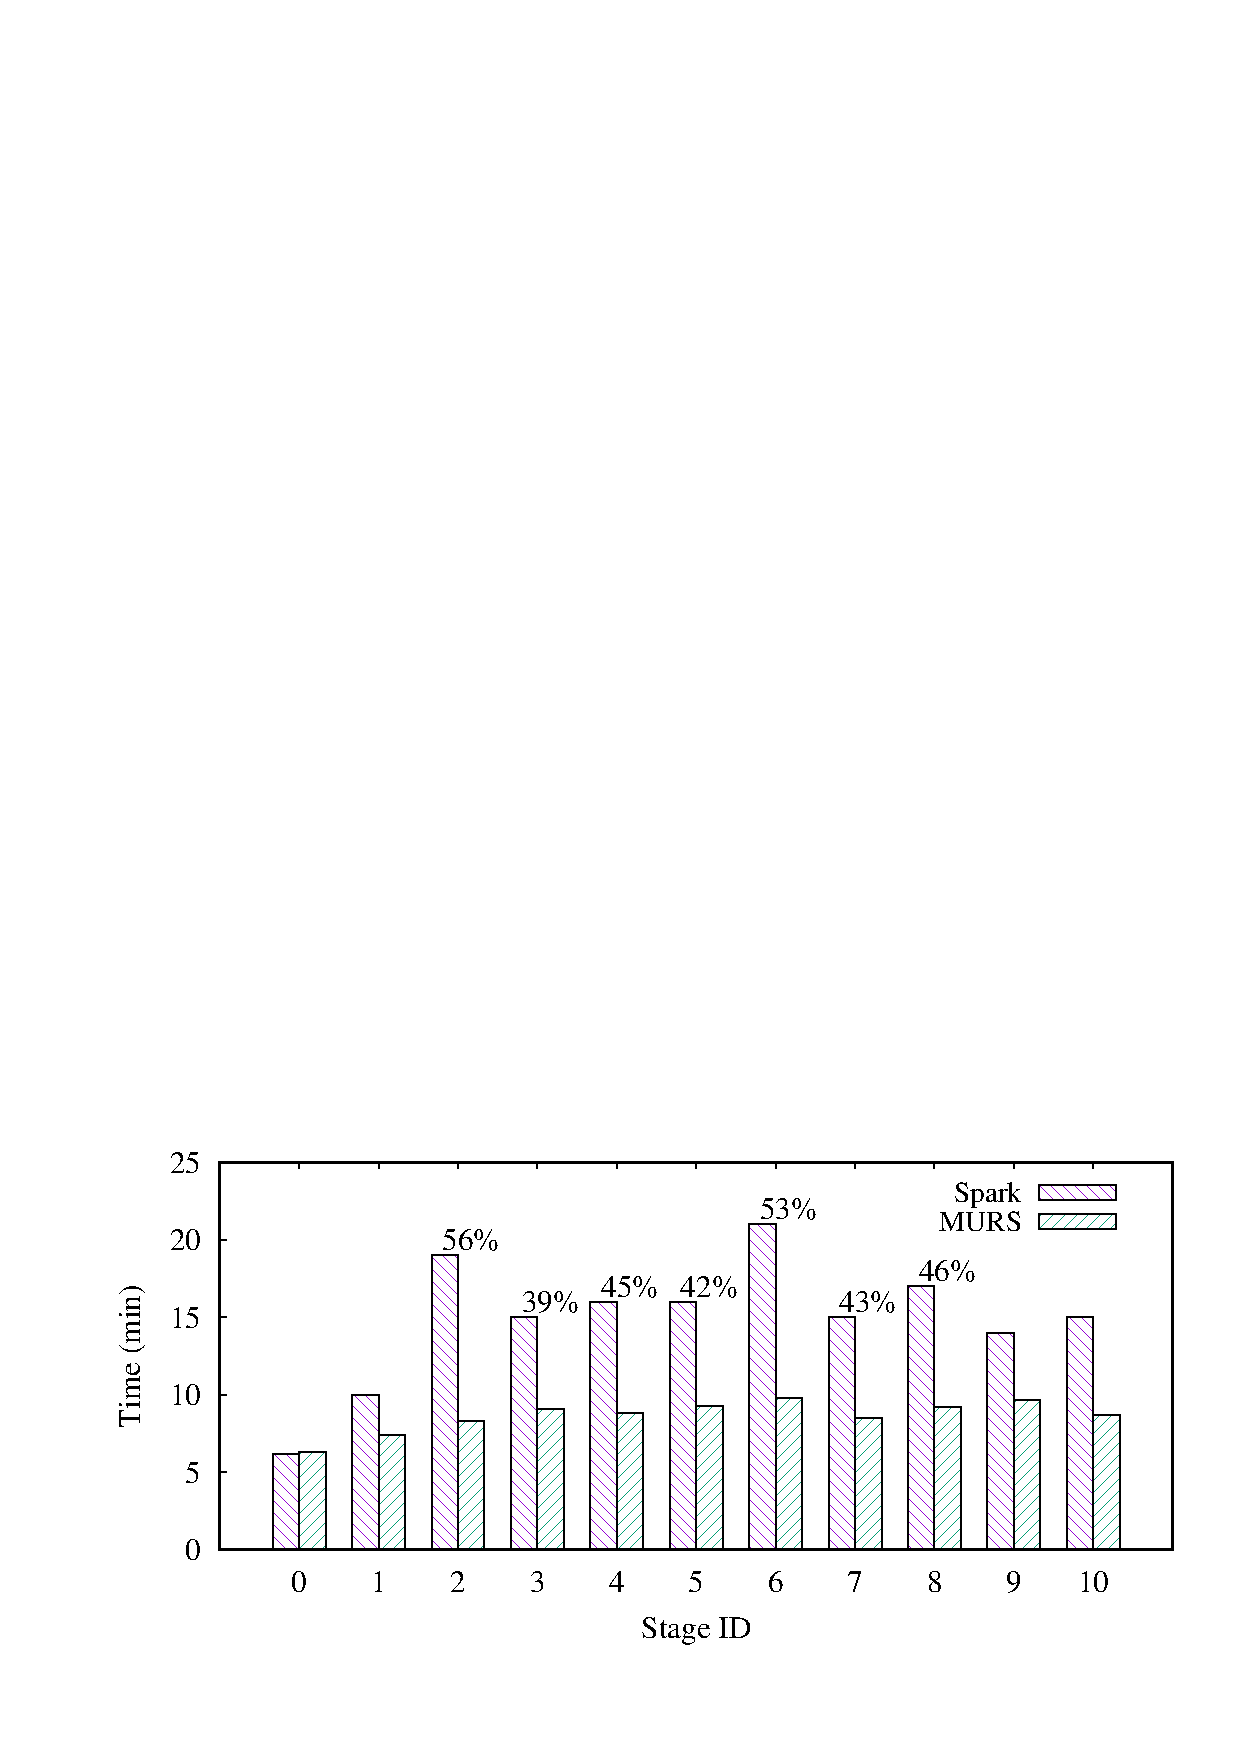
\includegraphics[width=0.45\textwidth]{pr-stagetime.pdf}
\vspace{-2mm}
\caption{The Result of Each Stages in PageRank}
\vspace{-2mm}
\label{fig:pr-stagetime}
\end{figure}

The caching data cost constant memory space because the caching data has same lifetime in the job. While less execution memory space is accessible for shuffle operation, the same data objects will result in worse memory pressure and more frequently garbage collection. The improvement of PageRank in MURS is benefit from three points: GC reduction, spill avoidance  and stopping tasks.

\begin{figure}[!t]
\centering
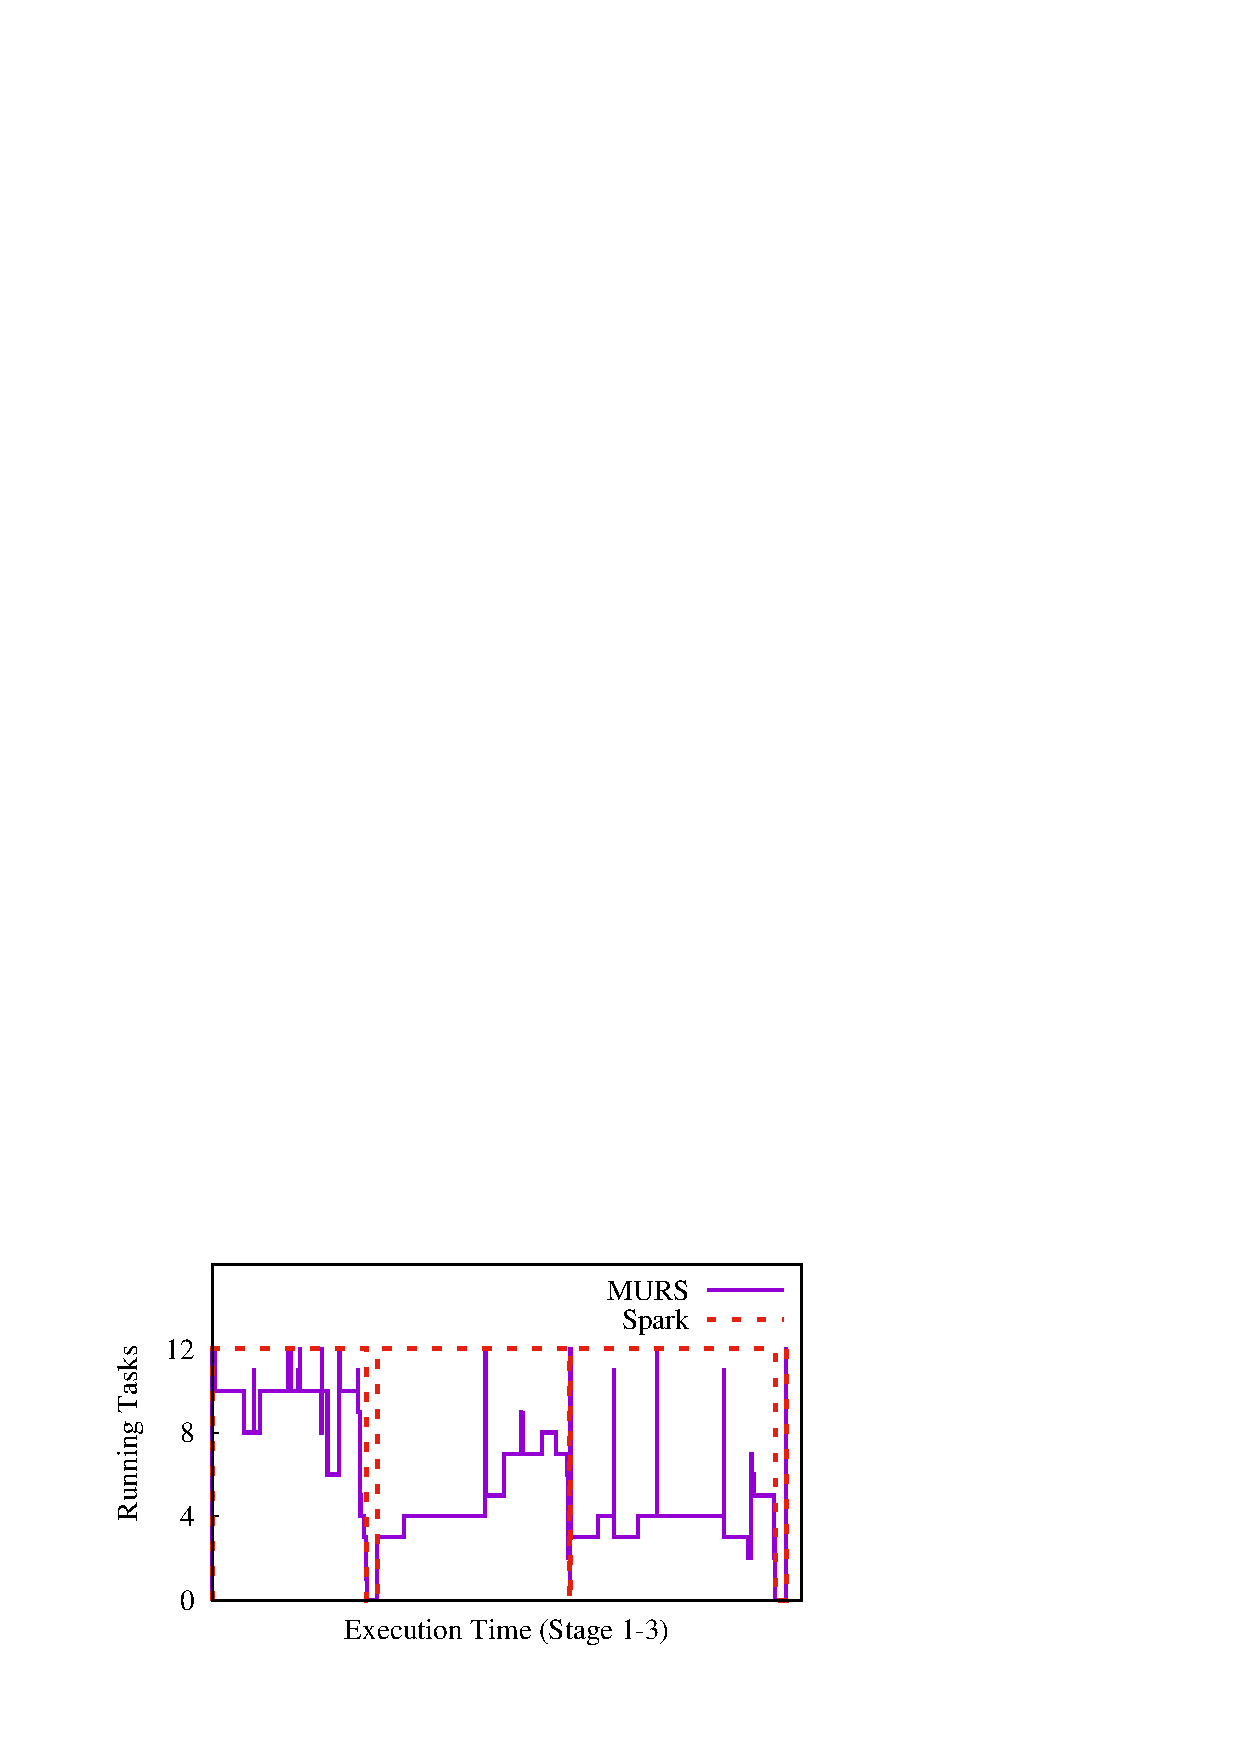
\includegraphics[width=0.35\textwidth]{pr-runtasks.pdf}
\vspace{-2mm}
\caption{The Number of Running Tasks in MURS}
\vspace{-2mm}
\label{fig:pr-runtasks}
\end{figure}

\textbf{Stopping tasks} The core scheduling in MURS is stopping parts of tasks to prevent heavy memory pressure, thus we firstly analysis the count of running tasks as shown in Figure~\ref{fig:pr-runtasks}. The first stage has no caching data but some shuffle buffers in memory. The shuffle buffer will be live in JVM heap until write to disk, thus they result in some memory pressure and our scheduler stop two tasks accordingly. When the job runs in after stages, caching data will stay in memory until the job complete. The heavy memory pressure result in more stopped tasks.

\begin{figure}[!t]
\centering
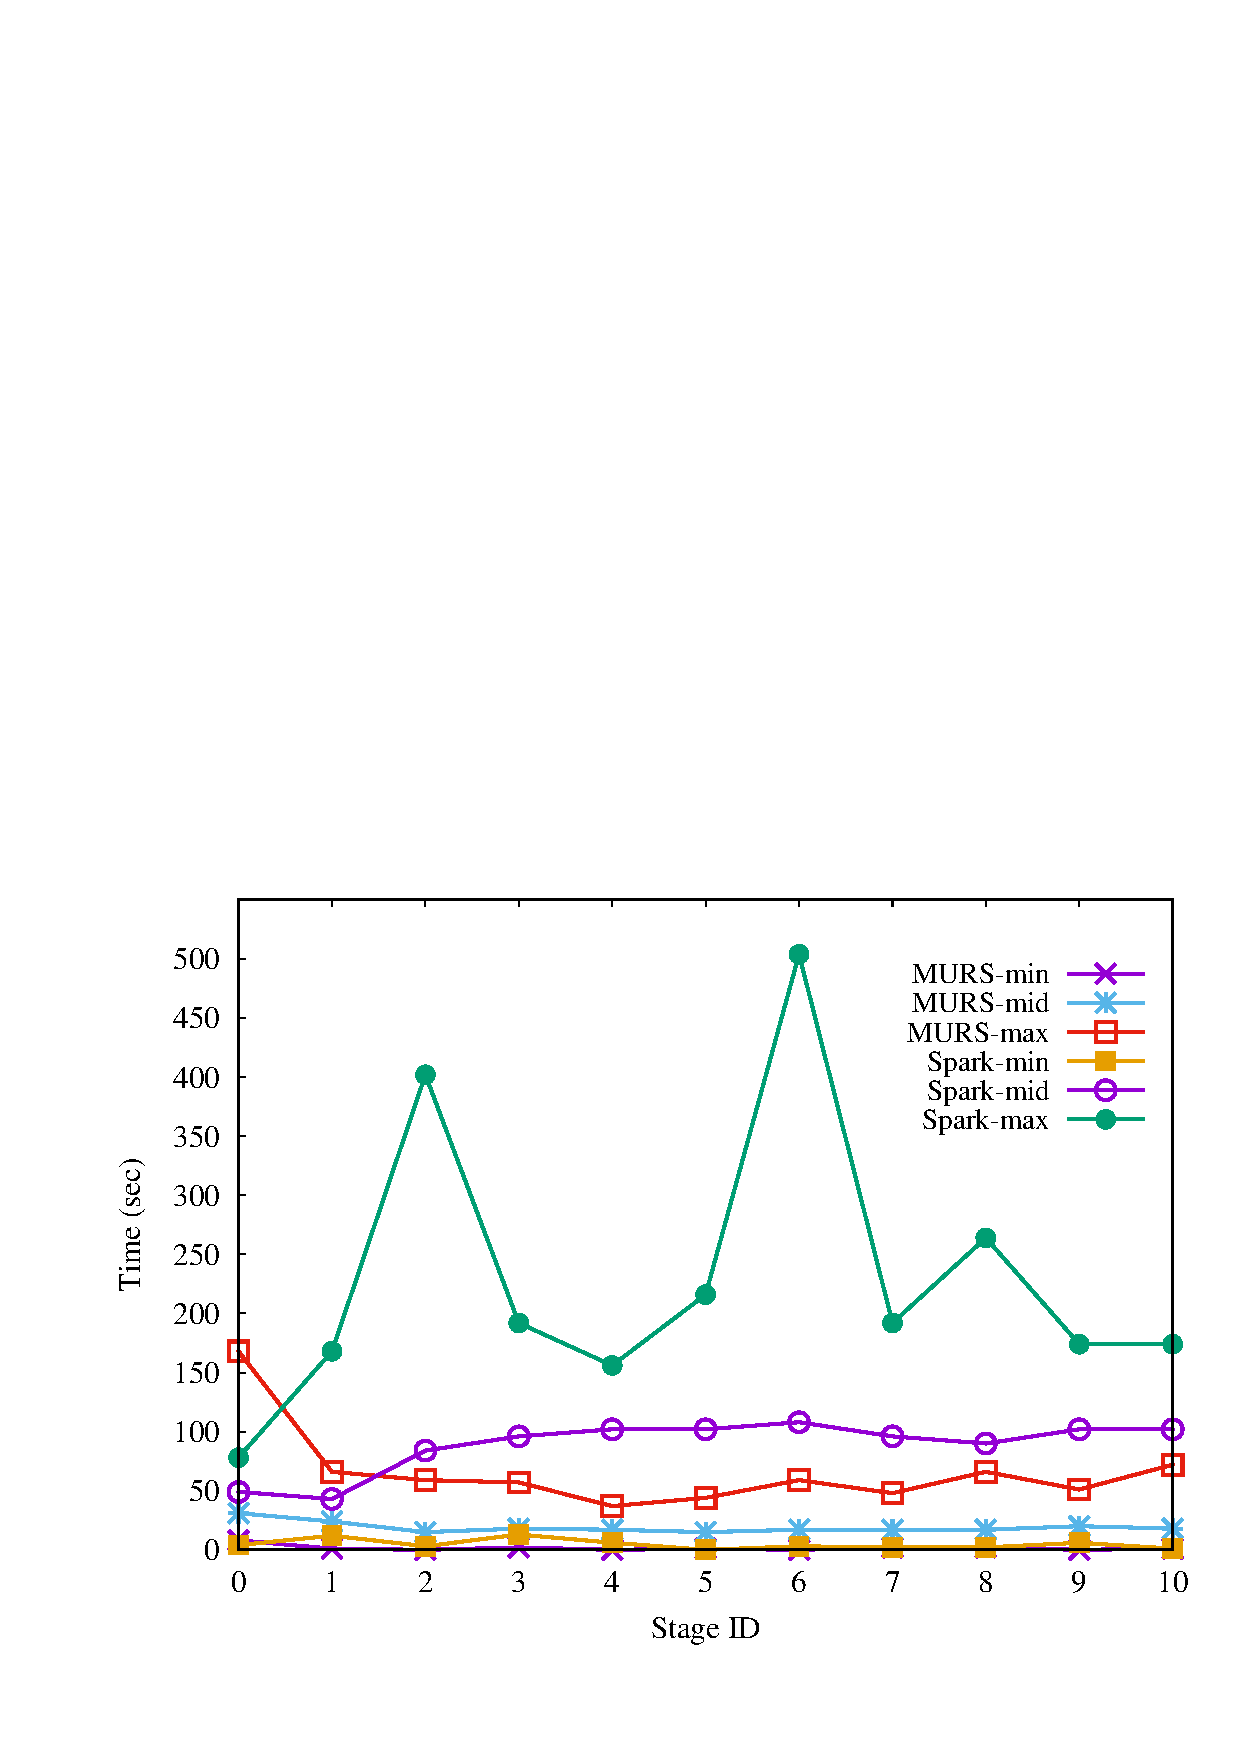
\includegraphics[width=0.45\textwidth]{pr-gc.pdf}
\vspace{-2mm}
\caption{The GC of Total Tasks in PageRank}
\vspace{-4mm}
\label{fig:pr-gc}
\end{figure}

\textbf{GC reduction} Each task suffers from different garbage collection, as shown in Figure~\ref{fig:pr-gc}. We compare the minimum, median and maximum of total tasks. Each guideline in MURS is better than Spark. The median of garbage collection time in MURS has the speed up of 5.5x. The reduction of garbage collection can be more cleared with the peak execution memory of each task. Peak execution memory of each task is 457MB/533MB/868MB(min/mid/max) in MURS, and 369MB/493MB/597MB(min/mid/max) in Spark. As MURS stop some tasks to avoid the cost of memory space which will be occupied for a long time, other running tasks has more execution memory. While the same memory space is provided for less running tasks, the peak execution memory of each tasks will be high. If the peak execution memory is high, tasks can run without heavy memory pressure because less garbage collection will occur. After the running tasks release their occupied space, stopped tasks can also improve their peak execution memory. Thus the memory pressure in MURS is lighter than Spark, and more execution memory slow down the heavy garbage collection essentially.

We can also get the conclusion that the straggler can be avoided in some way. The max garbage collection time and the average time is much near in MURS but fluctuating serious in Spark. As the time of garbage collection makes up the important part of execution time, tasks with long period of garbage collection will have long execution time. If the execution time of one task exceeds the average time of completed tasks, we regard it as an straggler. Thus MURS will have low probability to produce the straggler.

\begin{table}[!t]
\small
\centering
\begin{tabular}{| c | c | c | c | c | c | c | c |}

\hline
\multirow{2}{*}{} & \multirow{2}{*}{Stage} & \multicolumn{3}{| c |}{Spill Percent} & \multicolumn{3}{| c |}{Spill Size (MB)} \\
\cline{3-8}
 & & total & spill & percent & min & mid & max \\
\hline
\multirow{2}{*}{Spark} & stage6 & 300 & 185 & 62\% & 0 & 370 & 480 \\
\cline{2-8}
 & stage1 & 300 & 52 & 17\% & 0 & 0 & 471 \\
\hline
\multirow{2}{*}{MURS} & stage6 & 300 & 0 & 0\% & - & - & -  \\
\cline{2-8}
 & stage1 & 300 & 1 & 1\% & 0 & 0 & 399 \\
\hline

\hline
\end{tabular}
\vspace{-2mm}
\caption{Spill Tasks in MURS and Spark} 
\vspace{-4mm}
\label{table:pr-spill}
\end{table}

\textbf{Spill avoidance} Spark has several spill tasks in each stage, and only one stage of MURS has spill tasks, as shown in Table~\ref{table:pr-spill}. No matter in the first stage or other stages, most tasks can avoid spilling in MURS although they would spill in Spark. The fundamental reason is also more execution memory. MURS has the spill computing algorithm to avoid spilling. After stopping tasks, remain space are enough to running tasks is just the goal of MURS. While multi launch is available, the spill computing algorithm is more functional to control the running tasks. We notice that spill also appear in MURS, there are two points here: 1) estimating the remaining using space of one running task is not usually accurate; 2) the available memory space of one thread in JVM is limited (1/2N at least and 1/N at most while N is the number of running threads in JVM). Spill can result in expensive disk IO, thus the performance can be better.% in MURS.

\subsection{Multi-tenant}

Spark JobServer can provide multi-tenant for Spark. We submit both WordCount and PageRank to the Spark JobServer to test the performance of MURS in multi-tenant. We set the number of iterations to be 3 in PageRank, when the WordCount completes, PageRank usually complete the second stage. The result is shown in Figure~\ref{fig:mul-exec}. The execution time of WordCount decreased 28\% but at the same time the execution time of PageRank increased 26\%. After WordCount is complete, the execution of PageRank can be decreased to 58\%. We should notice that, when the WordCount is complete the PageRank runs both in Stage 2.

In the first stage, tasks in PR and WC are both \textit{ShuffleMapTask} which result in memory pressure through the shuffle buffer in shuffle writer. However, the function APIs in PR is \textit{groupBykey} which is a non-aggregation, it increases the size of shuffle buffer for each processed record. The function APIs in WC is \textit{reduceByKey} which is an aggregation, it increases the size of shuffle buffer only when the \textit{K} of processed record has never appeared. Obviously, the tasks in PR belong to linear while the tasks in WC belong to sub-linear. Our scheduler will stop the tasks of PR to prevent the heavy memory pressure, thus the tasks of WC can have less execution time. The pity is that the waiting time of stopped tasks increased much. Fortunately, as WC completes early, the third stage (Stage 2) in MURS suffer much less memory pressure, and the performance improves more. This is much important in multi-tenant, not only the tasks with heavy influence on memory pressure can execute more quickly, but also these tasks with light influence can avoid the memory pressure. The service of all tenant, which means PR and WC, can be better.

\end{comment}



\section{Related Work}

%Related works of this paper include these aspects:

% 机器学习在GPU性能分析上的应用实例。完全用机器学习预测和分析IPDPS16、HPCA15;
% 在AM模型上使用机器学习ICPE15。
% 另外需要提一下ML在特征工程上的重要性工作。

%Machine Learning in GPU performance analysis~\cite{nguyen:yak}. 

%Feature engineering in ML is also the basis of our work.

% 传统的性能分析模型的应用实例,通用模型方面,GPU架构HPCA11、应用本身的性能指标DATE16、应用的优化措施分析PPoPP12; 
% 专用模型方面,稀疏矩阵CC15、程序并行性ICPPW12、程序中判断条件的性能CCPE13
% 等。

%Analytical Model in GPU performance analysis is built on general cases or proprietary cases.
%General cases:
%architecture of GPU system. For example, work 1; work 2.
%optimization of GPU application. For example, work 3.
%runtime metrics of GPU applications. For example, work 4.
%Proprietary cases:
%SPMV; Parallelism; Conditions in instructions.

There is plenty of work on performance evaluation of GPU application, including traditional performance analysis models(AM) and machine learning-based approaches(ML). AM can be classified into general models and specific models. General models are generally applicable to any GPU program or kernel, and provide a comprehensive assessments, while specific models are for specific GPU programs or provide assessment for part of GPU architecture.

Zhang and Owens~\cite{Zhang2011A} propose a quantitative performance analysis model from the perspective of GPU architecture, in which they modele the execution time spent on the instruction pipeline, shared memory, and global memory, to find performance bottleneck of GPU application. Sim et al.~\cite{Sim2012A} present an analysis model from the perspective of application optimization methods. They classify the methods into four aspects and put forward four potential benefit metrics: B$_{itilp}$, B$_{memlp}$, B$_{fp}$, B$_{serial}$, to guide application performance optimization. Bombieri et al.~\cite{Bombieri2016A} propose a fine-grained performance model based on the performance metrics of GPU application, such as synchronization, thread divergence, load balancing, L1/L2, shared memory efficiency. The model rely on micro-benchmarks and several optimization criteria to estimate the potential performance of the application.

As for specific models, some researches are on specific GPU application. Guo and Wang~\cite{Guo2015Accurate} propose an analytical approach to predict the kernel execution time of sparse matrix-vector multiplications. Su et al.~\cite{Su2015An} present a performance analysis model for 3D stencil calculations based on the data transfer at different stages of the GPU memory hierarchy. Some researches focuses on one kind of GPU applications, for example, an analytic model that focuses on memory-bound applications is discribed in~\cite{Ma2012A}. Models for only one aspect of GPU also exist. Konstantinidis and Cotronis~\cite{Konstantinidis2016A} describe a performance evaluation for measuring the memory bandwidth of fast on-chip memories of GPU.

Traditional performance analysis models, although accurate, often require a detailed understanding of the hardware architecture, and they often rely on simulators or profiling tools to collect information, which is time-consuming. More and more researches use machine learning approaches to carry out performance evaluation.

Wu et al.~\cite{Wu2015GPGPU} describe a GPU performance and power estimation model, using machine learning method to explore the design space for different hardware configurations, and use the performance values in one configuration to predict performance and power in other configurations. Madougou et al.~\cite{Madougou2016A} present a statistical method for performance analysis based on hardware performance counters, using random forest algorithms combined with PCA (principal component analysis) and regression methods to identify performance bottlenecks and predict performance of GPU applications.

Performance evaluation based on machine learning is simple and easy to use, but its accuracy can not be guaranteed since it strongly depends on the training data sets, and feature selection is also very important. Didona et al.~\cite{Didona2015Enhancing} combine traditional analysis model with machine learning method, taking AM as an individual, and compares it with ML-based modeling to improve the robustness of performance prediction. But this method is not for GPU applications.

In our work, we combine machine learning approach with analysis model to conduct the performance evaluation. The process is divided into two stages. In the first stage, machine learning method is used to train and obtain the most influential features on GPU application execution time, and the features are sorted based on the degree of the influence. In the second stage we use the analysis model to analyze these features and identify the performance bottleneck.


\section{Conclusion}

In order to mitigate the memory pressure in current data processing systems for service, this paper analyzes the memory usage characters of variety function APIs provided by these systems and build three coarse grained models to classify them, then proposes memory usage rate as a uniform criterion to mark the influence of one task on memory pressure. The memory usage rate based scheduler called MURS can suspend these tasks resulting in heave memory pressure, and speed up these tasks with light memory pressure. MURS can be implemented in most data processing systems.

%\section{Introduction}
% no \IEEEPARstart
%This demo file is intended to serve as a ``starter file''
%for IEEE conference papers produced under \LaTeX\ using
%IEEEtran.cls version 1.7 and later.

%All manuscripts must be in English. These guidelines include complete descriptions of the fonts, spacing, and related information for producing your proceedings manuscripts. Please follow them and if you have any questions, direct them to the production editor in charge of your proceedings at Conference Publishing Services (CPS): Phone +1 (714) 821-8380 or Fax +1 (714) 761-1784.
% You must have at least 2 lines in the paragraph with the drop letter
% (should never be an issue)

%\subsection{Subsection Heading Here}
%Subsection text here.


%\subsubsection{Subsubsection Heading Here}
%Subsubsection text here.

%\section{Type style and Fonts}
%Wherever Times is specified, Times Roman or Times New Roman may be used. If neither is available on your system, please use the font closest in appearance to Times. Avoid using bit-mapped fonts if possible. True-Type 1 or Open Type fonts are preferred. Please embed symbol fonts, as well, for math, etc.


% An example of a floating figure using the graphicx package.
% Note that \label must occur AFTER (or within) \caption.
% For figures, \caption should occur after the \includegraphics.
% Note that IEEEtran v1.7 and later has special internal code that
% is designed to preserve the operation of \label within \caption
% even when the captionsoff option is in effect. However, because
% of issues like this, it may be the safest practice to put all your
% \label just after \caption rather than within \caption{}.
%
% Reminder: the "draftcls" or "draftclsnofoot", not "draft", class
% option should be used if it is desired that the figures are to be
% displayed while in draft mode.
%
%\begin{figure}[!t]
%\centering
%\includegraphics[width=2.5in]{myfigure}
% where an .eps filename suffix will be assumed under latex, 
% and a .pdf suffix will be assumed for pdflatex; or what has been declared
% via \DeclareGraphicsExtensions.
%\caption{Simulation Results}
%\label{fig_sim}
%\end{figure}

% Note that IEEE typically puts floats only at the top, even when this
% results in a large percentage of a column being occupied by floats.


% An example of a double column floating figure using two subfigures.
% (The subfig.sty package must be loaded for this to work.)
% The subfigure \label commands are set within each subfloat command, the
% \label for the overall figure must come after \caption.
% \hfil must be used as a separator to get equal spacing.
% The subfigure.sty package works much the same way, except \subfigure is
% used instead of \subfloat.
%
%\begin{figure*}[!t]
%\centerline{\subfloat[Case I]\includegraphics[width=2.5in]{subfigcase1}%
%\label{fig_first_case}}
%\hfil
%\subfloat[Case II]{\includegraphics[width=2.5in]{subfigcase2}%
%\label{fig_second_case}}}
%\caption{Simulation results}
%\label{fig_sim}
%\end{figure*}
%
% Note that often IEEE papers with subfigures do not employ subfigure
% captions (using the optional argument to \subfloat), but instead will
% reference/describe all of them (a), (b), etc., within the main caption.


% An example of a floating table. Note that, for IEEE style tables, the 
% \caption command should come BEFORE the table. Table text will default to
% \footnotesize as IEEE normally uses this smaller font for tables.
% The \label must come after \caption as always.
%
%\begin{table}[!t]
%% increase table row spacing, adjust to taste
%\renewcommand{\arraystretch}{1.3}
% if using array.sty, it might be a good idea to tweak the value of
% \extrarowheight as needed to properly center the text within the cells
%\caption{An Example of a Table}
%\label{table_example}
%\centering
%% Some packages, such as MDW tools, offer better commands for making tables
%% than the plain LaTeX2e tabular which is used here.
%\begin{tabular}{|c||c|}
%\hline
%One & Two\\
%\hline
%Three & Four\\
%\hline
%\end{tabular}
%\end{table}


% Note that IEEE does not put floats in the very first column - or typically
% anywhere on the first page for that matter. Also, in-text middle ("here")
% positioning is not used. Most IEEE journals/conferences use top floats
% exclusively. Note that, LaTeX2e, unlike IEEE journals/conferences, places
% footnotes above bottom floats. This can be corrected via the \fnbelowfloat
% command of the stfloats package.



%\section{Conclusion}
%The conclusion goes here. this is more of the conclusion

% conference papers do not normally have an appendix


% use section* for acknowledgement
%\section*{Acknowledgment}


%The authors would like to thank somebody and somebody. The work is provided by 


% trigger a \newpage just before the given reference
% number - used to balance the columns on the last page
% adjust value as needed - may need to be readjusted if
% the document is modified later
%\IEEEtriggeratref{8}
% The "triggered" command can be changed if desired:
%\IEEEtriggercmd{\enlargethispage{-5in}}

% references section

% can use a bibliography generated by BibTeX as a .bbl file
% BibTeX documentation can be easily obtained at:
% http://www.ctan.org/tex-archive/biblio/bibtex/contrib/doc/
% The IEEEtran BibTeX style support page is at:
% http://www.michaelshell.org/tex/ieeetran/bibtex/
%\bibliographystyle{IEEEtran}
% argument is your BibTeX string definitions and bibliography database(s)
%\bibliography{IEEEabrv,../bib/paper}
%
% <OR> manually copy in the resultant .bbl file
% set second argument of \begin to the number of references
% (used to reserve space for the reference number labels box)
%\begin{thebibliography}{1}

%\bibitem{IEEEhowto:kopka}
%H.~Kopka and P.~W. Daly, \emph{A Guide to \LaTeX}, 3rd~ed.\hskip 1em plus
%  0.5em minus 0.4em\relax Harlow, England: Addison-Wesley, 1999.

%\end{thebibliography}

\bibliographystyle{IEEEtran}
\bibliography{ref}


% that's all folks
\end{document}


